 % use font size 10pt for large document
% use font size  8pt for small document

\documentclass[a4,8pt,landscape]{extarticle}

\usepackage{paralist}
% PARAMETER TO GREY OUT TEXT
\usepackage{etoolbox}
\newtoggle{greytext}
%\toggletrue{greytext}
\togglefalse{greytext}

% PARAMETER TO SHORTEN DOCUMENT
\newtoggle{shortdocument}
\toggletrue{shortdocument}
%\togglefalse{shortdocument}

% DECREASE LINE SPACING IF REQUESTED
\iftoggle{shortdocument}{
\setlength{\baselineskip}{0pt}
\renewcommand{\baselinestretch}{0.00001}
% TODO: next time: (better, but i have to use other equations)
%\setlength{\baselineskip}{1pt}
%\setlength{\lineskiplimit}{-16pt}
}

% PAPER LAYOUT
\iftoggle{shortdocument}{
\usepackage[margin=0.25cm,twoside]{geometry}
}{
\usepackage[margin=0.5cm,twoside
% TODO: activate if needed,bindingoffset=9mm
]{geometry}
}

% LANDSCAPE PACKAGE
\usepackage{pdflscape}

% TODO: page numbering
\usepackage{fancyhdr}
\pagestyle{fancy}
\renewcommand{\headrulewidth}{0pt}
\fancyfoot[C]{{\setlength\fboxsep{3pt}
\vspace*{-0.55cm}\colorbox{white}{\scriptsize\thepage}}}
\setlength{\footskip}{4pt}

% COMMENTS (invisible)
\usepackage{comment}

% COLORS
\usepackage{color}
\usepackage[dvipsnames]{xcolor}

% COLOR SHORTCUTS
\iftoggle{greytext}{
\newcommand{\tcr}[1]{\textcolor{lighttext}{#1}}
\newcommand{\tcb}[1]{\textcolor{lighttext}{#1}}
\newcommand{\tcg}[1]{\textcolor{lighttext}{#1}}
\newcommand{\tcgr}[1]{\textcolor{lighttext}{#1}}
\newcommand{\tcp}[1]{\textcolor{lighttext}{#1}}
}{
\newcommand{\tcr}[1]{\textcolor{red}{#1}}
\newcommand{\tcb}[1]{\textcolor{blue}{#1}}
\newcommand{\tcg}[1]{\textcolor{green}{#1}}
\newcommand{\tcp}[1]{\textcolor{pink}{#1}}
\newcommand{\tcgr}[1]{\textcolor{gray}{#1}}
}
\newcommand{\bs}{\boldsymbol}

% MULTICOLUMN LAYOUT
\usepackage{multicol}
\iftoggle{shortdocument}{
\setlength\columnsep{10pt}
}{
\setlength\columnsep{20pt}
}
\setlength{\columnseprule}{0.1pt}
\iftoggle{greytext}{
\renewcommand{\columnseprulecolor}{\color{lighttext}}
}{
}

% PARAGRAPH LAYOUT
\setlength\parindent{0pt}	% indentation
\setlength\parskip{2pt}		% space between paragraphs

% LANGUAGE SETTINGS
%\usepackage[ngerman]{babel} % Silbentrennung (und Deutsche Titel)
\usepackage[utf8]{inputenc} % Umlaute

% FONTS
%\usepackage{mathpazo}
%\usepackage{helvet}
%\usepackage{fouriernc}
%\usepackage[varg]{txfonts}
%\usepackage{mathptmx}
%\usepackage[charter]{mathdesign}
%\usepackage[garamond]{mathdesign}
%\usepackage[utopia]{mathdesign}
%\usepackage{fourier}
% font kerning (load after specific font!)
\usepackage{microtype}

% CUSTOM FONT SIZES
\usepackage{relsize}

% FIGURE SETTINGS
\usepackage{pict2e} % load this before picture
\usepackage{picture}
\usepackage{graphicx}
\usepackage{adjustbox}
\usepackage{caption}
\usepackage{subcaption}

% TIKZ GRAPHICS
\usepackage{tikz}
\usetikzlibrary{calc,matrix,arrows,automata,fit,shapes.multipart}
\tikzset{% 
    arr/.style={%
        -latex
    }
}
\tikzset{%
    var/.style={%
    	circle,draw=black
    }
}
\tikzset{%
	fac/.style={%
		rectangle,draw=black,align=center
	}
}
\newcommand{\fadeoutarr}[2]{%
\draw[] (#1) edge 
        ($(#1)!0.45!(#2)$) edge [dotted] 
        ($(#1)!0.75!(#2)$)
}
\newcommand{\fadeinarr}[2]{%
\draw[] ($(#1)!0.45!(#2)$) edge[dotted] 
        ($(#1)!0.75!(#2)$) edge[arr] 
        (#2) }
        
\newcommand{\tfactor}[4]{
\node[fac] (#1) at (#2) {{\tiny #4}\\#3};
}
\newcommand{\tnode}[3]{
\node[var] (#1) at (#2) {#3};
}
\newcommand{\tedge}[2]{
\draw[] (#1) edge (#2);
}
\newcommand{\tarrow}[2]{
\draw[arr] (#1) edge (#2);
}
\usepackage{tikz-cd}

% SIMPLE TREES
\usepackage{qtree}

% PLOTS
\usepackage{pgfplots}
\pgfplotsset{compat=1.10}

% FLOAT SETTINGS
\usepackage{float}

% REFERENCING
\usepackage{hyperref}

% TABLES
\usepackage{booktabs} % nicer tables
\usepackage{makecell}
\usepackage{array} % custom column types
\usepackage{multirow} % span cells over multiple rows
\newcommand{\tabitem}{~~\llap{{\boldmath $\cdot$}}~} % items in tables

% LISTS
\usepackage{enumitem}
\setlist{noitemsep,topsep=0pt,parsep=0pt,partopsep=0pt,leftmargin=10pt}
\renewcommand\labelitemi{{\boldmath$\cdot$}}
\renewcommand\labelitemii{{\boldmath$\cdot$}}
\renewcommand\labelitemiii{{\boldmath$\cdot$}}
% advantages disadvantages
\newcommand\pro{\item[$+$]}
\newcommand\con{\item[$-$]}

% TIGHT CENTER ENVIRONMENT
\newenvironment{tightcenter}{%
  \begin{center}
  \vspace{-12pt}
}{
  \vspace{-12pt}
  \end{center}
}

% COMMAND TO ROTATE MATH SYMBOLS
\newcommand{\rot}[2]{\rotatebox[origin=c]{#1}{#2}}

% MATH (packages and settings)
\usepackage{blkarray}  		% matrix annotations
\usepackage[intlimits]{mathtools}
\usepackage{amsfonts}
\usepackage{bm}
\usepackage{amssymb}
\usepackage{wasysym}
\usepackage{ifsym}
\usepackage{dsfont}
\usepackage{resizegather} 	% resizing equations
\usepackage{oubraces}    	% special overlapping over/underbraces
\usepackage{scalerel}		% scaling of characters
\usepackage{cancel}			% crossing out of terms
\allowdisplaybreaks 		% allow page break in align* environment

% PROOF TREES
\usepackage{proof}
\inferLineSkip=4pt % adjust line skip between proofs

% PROOFS
\newcommand{\qed}{\hfill$\square$}
\newcommand{\contradiction}{\hfill$\lightning$}

% MATH HIGHLIGHTING
\newcommand{\mhl}[2]{\colorbox{#1}{$\displaystyle#2$}}
\newcommand{\mhlr}[1]{\mathhl{red}{#1}}
\newcommand{\mhlg}[1]{\mathhl{green}{#1}}
\newcommand{\mhlb}[1]{\mathhl{blue}{#1}}
\newcommand{\mhly}[1]{\mathhl{yellow}{#1}}

% CODE IN MATH
\newcommand{\mcode}[1]{{\normalfont\texttt{\textbf{#1}}}}

% COLOR IN MATH (without the bad behaviour of textcolor)
\makeatletter
\def\mc#1#{\@mc{#1}}
\def\@mc#1#2#3{%
  \protect\leavevmode
  \begingroup
    \color#1{#2}#3%
  \endgroup
}
\makeatother

\iftoggle{greytext}{
\definecolor{brilliantrose}{rgb}{1.0, 0.33, 0.64}
\newcommand{\mcr}[1]{\mc{lighttext}{#1}}
\newcommand{\mcg}[1]{\mc{lighttext}{#1}}
\newcommand{\mcb}[1]{\mc{lighttext}{#1}}
\newcommand{\mcy}[1]{\mc{lighttext}{#1}}
\newcommand{\mcp}[1]{\mc{lighttext}{#1}}
\newcommand{\mcw}[1]{\mc{white}{#1}}
\newcommand{\mcgr}[1]{\mc{lighttext}{#1}}
}{
\definecolor{brilliantrose}{rgb}{1.0, 0.33, 0.64}
\newcommand{\mcr}[1]{\mc{red}{#1}}
\newcommand{\mcg}[1]{\mc{green}{#1}}
\newcommand{\mcb}[1]{\mc{blue}{#1}}
\newcommand{\mcy}[1]{\mc{yellow}{#1}}
\newcommand{\mcp}[1]{\mc{brilliantrose}{#1}}
\newcommand{\mcw}[1]{\mc{white}{#1}}
\newcommand{\mcgr}[1]{\mc{gray}{#1}}
}

% ASYMPTOTIC NOTATIONS
\newcommand{\BigO}{\mathcal{O}}

% NUMBER SYSTEMS
\newcommand{\A}{\mathbb{A}}
\newcommand{\B}{\mathbb{B}}
\newcommand{\C}{\mathbb{C}}
\newcommand{\D}{\mathbb{D}}
\newcommand{\E}{\mathbb{E}}
\newcommand{\F}{\mathbb{F}}
\newcommand{\G}{\mathbb{G}}
\newcommand{\bbH}{\mathbb{H}}
\newcommand{\I}{\mathbb{I}}
\newcommand{\J}{\mathbb{J}}
\newcommand{\K}{\mathbb{K}}
\newcommand{\bbL}{\mathbb{L}}
\newcommand{\M}{\mathbb{M}}
\newcommand{\N}{\mathbb{N}}
\newcommand{\bbO}{\mathbb{O}}
\newcommand{\bbP}{\mathbb{P}}
\newcommand{\Q}{\mathbb{Q}}
\newcommand{\R}{\mathbb{R}}
\newcommand{\bbS}{\mathbb{S}}
\newcommand{\bbT}{\mathbb{T}}
\newcommand{\U}{\mathbb{U}}
\newcommand{\V}{\mathbb{V}}
\newcommand{\W}{\mathbb{W}}
\newcommand{\X}{\mathbb{X}}
\newcommand{\Y}{\mathbb{Y}}
\newcommand{\Z}{\mathbb{Z}}

% CALLICGRAPHIC SHORTCUTS
\newcommand{\cA}{\mathcal{A}}
\newcommand{\cB}{\mathcal{B}}
\newcommand{\cC}{\mathcal{C}}
\newcommand{\cD}{\mathcal{D}}
\newcommand{\cE}{\mathcal{E}}
\newcommand{\cF}{\mathcal{F}}
\newcommand{\cG}{\mathcal{G}}
\newcommand{\cH}{\mathcal{H}}
\newcommand{\cI}{\mathcal{I}}
\newcommand{\cJ}{\mathcal{J}}
\newcommand{\cK}{\mathcal{K}}
\newcommand{\cL}{\mathcal{L}}
\newcommand{\cM}{\mathcal{M}}
\newcommand{\cN}{\mathcal{N}}
\newcommand{\cO}{\mathcal{O}}
\newcommand{\cP}{\mathcal{P}}
\newcommand{\cQ}{\mathcal{Q}}
\newcommand{\cR}{\mathcal{R}}
\newcommand{\cS}{\mathcal{S}}
\newcommand{\cT}{\mathcal{T}}
\newcommand{\cU}{\mathcal{U}}
\newcommand{\cV}{\mathcal{V}}
\newcommand{\cW}{\mathcal{W}}
\newcommand{\cX}{\mathcal{X}}
\newcommand{\cY}{\mathcal{Y}}
\newcommand{\cZ}{\mathcal{Z}}

% BRACES
\newcommand{\set}[1]{\left\{ #1 \right\}}
\newcommand{\dset}[2]{\left\{ #1 \ \middle| \ #2 \right\}}
\newcommand{\alg}[1]{\left\langle #1 \right\rangle}
\newcommand{\card}[1]{\left\lvert #1 \right\rvert}
\newcommand{\length}[1]{\left\lvert #1 \right\rvert}
\newcommand{\abs}[1]{\left\lvert #1 \right\rvert}
\newcommand{\norm}[1]{\left\lVert #1 \right\rVert}
\newcommand{\scprod}[1]{\left\langle #1 \right\rangle}
\newcommand{\ceil}[1]{\left\lceil #1 \right\rceil}
\newcommand{\floor}[1]{\left\lfloor #1 \right\rfloor}
\newcommand{\linsys}[2]{\left[\ #1 \ \middle| \ #2 \ \right]}
\newcommand{\Sim}[1]{\text{Sim}\left( #1 \right)}
\newcommand{\Tr}[1]{\mathsf{Tr}\left( #1 \right)}
\newcommand{\sTr}[1]{\mathsf{Tr}( #1 )}

% BRACES SMALL (no adjusting)
\newcommand{\sset}[1]{\{ #1 \}}
\newcommand{\sdset}[2]{\{ #1 \ | \ #2 \}}
\newcommand{\salg}[1]{\langle #1 \rangle}
\newcommand{\scard}[1]{\lvert #1 \rvert}
\newcommand{\slength}[1]{\lvert #1 \rvert}
\newcommand{\sabs}[1]{\lvert #1 \rvert}
\newcommand{\snorm}[1]{\lVert #1 \rVert}
\newcommand{\sscprod}[1]{\langle #1 \rangle}
\newcommand{\sceil}[1]{\lceil #1 \rceil}
\newcommand{\sfloor}[1]{\lfloor #1 \rfloor}
\newcommand{\slinsys}[2]{[\ #1 \ | \ #2 \ ]}
\newcommand{\sSim}[1]{\text{Sim}( #1 )}

% OPERATORS
\newcommand{\conv}{\ensuremath *}

% EMPTY SET
\let\oldemptyset\emptyset
\let\emptyset\varnothing

% NOT IN SHORTCUT
\newcommand{\nin}{\not\in}

% DISJOINT UNION SYMBOL
\makeatletter
\def\moverlay{\mathpalette\mov@rlay}
\def\mov@rlay#1#2{\leavevmode\vtop{%
   \baselineskip\z@skip \lineskiplimit-\maxdimen
   \ialign{\hfil$\m@th#1##$\hfil\cr#2\crcr}}}
\newcommand{\charfusion}[3][\mathord]{
    #1{\ifx#1\mathop\vphantom{#2}\fi
        \mathpalette\mov@rlay{#2\cr#3}
      }
    \ifx#1\mathop\expandafter\displaylimits\fi}
\makeatother
\newcommand{\bigcupdot}{\charfusion[\mathop]{\bigcup}{\cdot}}
\newcommand{\cupdot}{\mathbin{\mathaccent\cdot\cup}}

% CUSTOM STATISTICS
\newcommand{\Prob}[2][]{P_{#1}\left( #2 \right)}
\newcommand{\cProb}[3][]{P_{#1}\left( #2 \,\middle|\, #3 \right)}
\newcommand{\Dist}[2]{#1\left( #2 \right)}
\newcommand{\cDist}[3]{#1\left( #2 \,\middle|\, #3 \right)}
\newcommand{\hProb}[2][]{\hat{P}_{#1}\left( #2 \right)}
\newcommand{\chProb}[2]{\hat{P}\left( #1 \,\middle|\, #2 \right)}
\newcommand{\Var}[2][]{\operatorname{Var}_{#1}\left[ #2 \right]}
\newcommand{\sd}[1]{\operatorname{sd}\left( #1 \right)}
\newcommand{\Exp}[2][]{{\mathbb{E}_{#1}}\left[ #2
\right]}
\newcommand{\cExp}[3][]{{\mathbb{E}}_{#1}\left[ #2
\,\middle|\, #3 \right]}
\newcommand{\hExp}[2][]{{\mathbb{\hat{E}}_{#1}}\left[ #2
\right]}
\newcommand{\chExp}[3][]{{\mathbb{\hat{E}}}_{#1}\left[ #2
\,\middle|\, #3 \right]}
\newcommand{\Corr}[1]{\operatorname{Corr}\left[ #1 \right]}
\newcommand{\Cov}[1]{\operatorname{Cov}\left(#1 \right)}
\newcommand{\MSE}[2][]{\operatorname{MSE}_{#1}\left[ #2 \right]}
\newcommand{\riid}{\stackrel{\text{\tiny i.i.d.}}{\sim}}
\newcommand{\approxsim}{\stackrel{\text{approx.}}{\sim}}
\newcommand{\ind}[1]{\mathds{1}_{\set{#1}}}
\newcommand{\eqiid}{\stackrel{\text{\tiny i.i.d.}}{=}}
\newcommand{\eqind}{\stackrel{\text{\tiny ind.}}{=}}

% BAYESIAN NETWORKS
\newcommand{\indep}{\perp}
\newcommand{\given}{\,\,|\,\,}
\newcommand{\Pa}{\mathbf{Pa}}
\newcommand{\dsep}[2]{\operatorname{d-sep}\left( #1 \,\middle|\, #2 \right)}

% RANDOM VARIABLES
\newcommand{\rA}{A}
\newcommand{\rB}{B}
\newcommand{\rC}{C}
\newcommand{\rD}{D}
\newcommand{\rE}{E}
\newcommand{\rF}{F}
\newcommand{\rG}{G}
\newcommand{\rH}{H}
\newcommand{\rI}{I}
\newcommand{\rJ}{J}
\newcommand{\rK}{K}
\newcommand{\rL}{L}
\newcommand{\rM}{M}
\newcommand{\rN}{N}
\newcommand{\rO}{O}
\newcommand{\rP}{P}
\newcommand{\rQ}{Q}
\newcommand{\rR}{R}
\newcommand{\rS}{S}
\newcommand{\rT}{T}
\newcommand{\rU}{U}
\newcommand{\rV}{V}
\newcommand{\rW}{W}
\newcommand{\rX}{X}
\newcommand{\rY}{Y}
\newcommand{\rZ}{Z}

% RANDOM VECTORS
% declares a custom italic bold alphabet for random vectors
\DeclareMathAlphabet{\mathbfit}{OML}{cmm}{b}{it}
\newcommand{\rvA}{\mathbfit{A}}
\newcommand{\rvB}{\mathbfit{B}}
\newcommand{\rvC}{\mathbfit{C}}
\newcommand{\rvD}{\mathbfit{D}}
\newcommand{\rvE}{\mathbfit{E}}
\newcommand{\rvF}{\mathbfit{F}}
\newcommand{\rvG}{\mathbfit{G}}
\newcommand{\rvH}{\mathbfit{H}}
\newcommand{\rvI}{\mathbfit{I}}
\newcommand{\rvJ}{\mathbfit{J}}
\newcommand{\rvK}{\mathbfit{K}}
\newcommand{\rvL}{\mathbfit{L}}
\newcommand{\rvM}{\mathbfit{M}}
\newcommand{\rvN}{\mathbfit{N}}
\newcommand{\rvO}{\mathbfit{O}}
\newcommand{\rvP}{\mathbfit{P}}
\newcommand{\rvQ}{\mathbfit{Q}}
\newcommand{\rvR}{\mathbfit{R}}
\newcommand{\rvS}{\mathbfit{S}}
\newcommand{\rvT}{\mathbfit{T}}
\newcommand{\rvU}{\mathbfit{U}}
\newcommand{\rvV}{\mathbfit{V}}
\newcommand{\rvW}{\mathbfit{W}}
\newcommand{\rvX}{\mathbfit{X}}
\newcommand{\rvY}{\mathbfit{Y}}
\newcommand{\rvZ}{\mathbfit{Z}}

% MACHINE LEARNING
\newcommand{\Risk}[1]{R\left(#1\right)}
\newcommand{\empRisk}[1]{\widehat{R}\left(#1\right)}

% ACCENTS
% TODO: fix this, make spacing nice
\newcommand*{\Hm}{\mathsf{H}}
\newcommand*{\T}{\mathsf{T}}
%\newcommand*{\T}{\mkern-1mu{}_{}^{\scriptscriptstyle\top}\mkern-4mu}
\newcommand*{\Rev}{\mathsf{R}}
\newcommand{\conj}[1]{\overline{ #1 }}

% CUSTOM ALPHABETS
\renewcommand{\S}{\Sigma}
\newcommand{\Ss}{\Sigma^*}
\newcommand{\Sp}{\Sigma^+}
\newcommand{\Sbool}{\Sigma_{\text{bool}}}
\newcommand{\Ssbool}{(\Sigma_{\text{bool}})^*}
\newcommand{\Slogic}{\Sigma_{\text{logic}}}
\newcommand{\Sslogic}{(\Sigma_{\text{logic}})^*}
\newcommand{\Slat}{\Sigma_{\text{lat}}}
\newcommand{\Sslat}{(\Sigma_{\text{lat}})^*}
\newcommand{\Stastatur}{\Sigma_{\text{Tastatur}}}
\newcommand{\Sstastatur}{(\Sigma_{\text{Tastatur}})^*}
\newcommand{\Sm}{\Sigma_{m}}
\newcommand{\Ssm}{\Sigma_{m}^*}
\newcommand{\ZO}{\{0,1\}}
\newcommand{\ZOs}{\{0,1\}^*}
\newcommand{\hdelta}{\hat\delta}

% OPERATORS
% TODO: Should I design these as braces?
\DeclareMathOperator{\id}{\text{id}}
\DeclareMathOperator{\Kon}{\text{Kon}}
\DeclareMathOperator{\cost}{\text{cost}}
\DeclareMathOperator{\goal}{\text{goal}}
\DeclareMathOperator{\Opt}{\text{Opt}}
\DeclareMathOperator{\Bin}{\text{Bin}}
\DeclareMathOperator{\Nummer}{\text{Nummer}}
\DeclareMathOperator{\Prim}{\text{Prim}}
\DeclareMathOperator{\Kl}{\text{Kl}}
\DeclareMathOperator{\lcm}{lcm}
\DeclareMathOperator{\glb}{glb}
\DeclareMathOperator{\lub}{lub}
\DeclareMathOperator{\im}{im}
\DeclareMathOperator{\ord}{ord}
\DeclareMathOperator{\rank}{rank}
\DeclareMathOperator{\spn}{span}
\DeclareMathOperator{\Cost}{Cost}
\DeclareMathOperator{\order}{order}
\DeclareMathOperator{\dist}{dist}
\DeclareMathOperator{\cond}{cond}
\DeclareMathOperator{\nnz}{nnz}
\DeclareMathOperator{\sign}{sign}
\DeclareMathOperator{\Count}{Count}
\DeclareMathOperator{\Spur}{Spur}
\DeclareMathOperator{\triu}{triu}
\DeclareMathOperator{\cumsum}{cumsum}
\DeclareMathOperator{\vectorize}{vectorize}
\DeclareMathOperator{\matrixfy}{matrixfy}
\DeclareMathOperator{\circul}{circul}
\DeclareMathOperator{\dft}{dft}
\DeclareMathOperator{\invdft}{invdft}
\DeclareMathOperator{\ones}{ones}
\DeclareMathOperator{\arcsinh}{arcsinh}
\DeclareMathOperator{\arccosh}{arccosh}
\DeclareMathOperator{\arctanh}{arctanh}
\let\division\div
\renewcommand\div{\operatorname{div}}
\DeclareMathOperator{\cis}{cis}
\DeclareMathOperator{\grad}{grad}
\DeclareMathOperator{\Hess}{Hess}
\newcommand{\laplace}{\Delta}
\DeclareMathOperator*{\argmin}{arg\,min}
\DeclareMathOperator*{\argmax}{arg\,max}
\DeclareMathOperator{\odd}{odd}
\DeclareMathOperator{\even}{even}
\DeclareMathOperator{\Proj}{Proj}
\DeclareMathOperator{\softmax}{\text{softmax}}
\DeclareMathOperator{\ReLU}{\text{ReLU}}
\DeclareMathOperator{\pmi}{\text{pmi}}

% TODO: fix these operator braces
% TODO: think about which ones should have braces
% and which one shouldn't. E.g., a function might need derivatives '
% or it might be used without argument, just in compositions \circ
\newcommand{\diag}{\text{diag}}

% CRYPTOGRAPHY
\DeclareMathOperator{\concat}{ || }
\DeclareMathOperator{\Enc}{Enc}
\DeclareMathOperator{\Dec}{Dec}
\DeclareMathOperator{\Gen}{Gen}
\DeclareMathOperator{\Tag}{Tag}
\DeclareMathOperator{\Vrfy}{Vrfy}
\DeclareMathOperator{\MAC}{\text{MAC}}
\newcommand{\AdvPRG}[2][]{\text{Adv}_{\text{PRG}}\left[ #2 \right]}
\newcommand{\yes}{\text{yes}}
\newcommand{\no}{\text{no}}
\newcommand{\forallPPTTM}{%
\underset{\mathclap{\substack{\text{\tiny prob. poly-}\\
\text{\tiny time TM}}}}{\forall}}
\newcommand{\forallPTAdv}{%
\underset{\mathclap{\substack{\text{\tiny poly-time}\\
\text{\tiny Adversaries}}}}{\forall}}

% OPERATORS (OVERRIDDEN)
\renewcommand\Re{\operatorname{Re}}
\renewcommand\Im{\operatorname{Im}}

% RELATIONAL ALGEBRA
\renewcommand{\setminus}{-} 
\DeclareMathOperator{\dom}{dom}
\DeclareMathOperator{\sch}{sch}
\newcommand{\dto}{\stackrel{\bullet}{\to}}
%\newcommand{\join}{\bowtie}
%\newcommand{\lojoin}{\,{\tiny \textifsym{d|><|}}\,}
%\newcommand{\rojoin}{\,{\tiny \textifsym{|><|d}}\,}
%\newcommand{\fojoin}{\,{\tiny \textifsym{d|><|d}}\,}
%\newcommand{\lsjoin}{\ltimes}
%\newcommand{\rsjoin}{\rtimes}

\newcommand{\fojoin}{
\,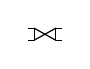
\begin{tikzpicture}%
% bowtie - X
\draw[line width=0.15mm,line cap=round] (0,0) -- (1.8ex,1ex);
\draw[line width=0.15mm,line cap=round] (0,1ex) -- (1.8ex,0ex);
% bowtie - side left
\draw[line width=0.15mm,line cap=round] (0,0) -- (0,1ex);
% bowtie - side right
\draw[line width=0.15mm,line cap=round] (1.8ex,0) -- (1.8ex,1ex);
% left wedges
\draw[line width=0.15mm] (0,0) -- (-0.5ex,0);
\draw[line width=0.15mm] (0,1ex) -- (-0.5ex,1ex);
% right wedges
\draw[line width=0.15mm] (1.8ex,0) -- (2.3ex,0);
\draw[line width=0.15mm] (1.8ex,1ex) -- (2.3ex,1ex);
\end{tikzpicture}\,
}

\newcommand{\join}{
\,
\begin{tikzpicture}%
% bowtie - X
\draw[line width=0.15mm,line cap=round] (0,0) -- (1.8ex,1ex);
\draw[line width=0.15mm,line cap=round] (0,1ex) -- (1.8ex,0ex);
% bowtie - side left
\draw[line width=0.15mm,line cap=round] (0,0) -- (0,1ex);
% bowtie - side right
\draw[line width=0.15mm,line cap=round] (1.8ex,0) -- (1.8ex,1ex);
\end{tikzpicture}\,
}

\newcommand{\lojoin}{
\,
\begin{tikzpicture}%
% bowtie - X
\draw[line width=0.15mm,line cap=round] (0,0) -- (1.8ex,1ex);
\draw[line width=0.15mm,line cap=round] (0,1ex) -- (1.8ex,0ex);
% bowtie - side left
\draw[line width=0.15mm,line cap=round] (0,0) -- (0,1ex);
% bowtie - side right
\draw[line width=0.15mm,line cap=round] (1.8ex,0) -- (1.8ex,1ex);
% left wedges
\draw[line width=0.15mm] (0,0) -- (-0.5ex,0);
\draw[line width=0.15mm] (0,1ex) -- (-0.5ex,1ex);
\end{tikzpicture}\,
}

\newcommand{\rojoin}{
\,
\begin{tikzpicture}%
% bowtie - X
\draw[line width=0.15mm,line cap=round] (0,0) -- (1.8ex,1ex);
\draw[line width=0.15mm,line cap=round] (0,1ex) -- (1.8ex,0ex);
% bowtie - side left
\draw[line width=0.15mm,line cap=round] (0,0) -- (0,1ex);
% bowtie - side right
\draw[line width=0.15mm,line cap=round] (1.8ex,0) -- (1.8ex,1ex);
% right wedges
\draw[line width=0.15mm] (1.8ex,0) -- (2.3ex,0);
\draw[line width=0.15mm] (1.8ex,1ex) -- (2.3ex,1ex);
\end{tikzpicture}\,
}

\newcommand{\lsjoin}{
\,
\begin{tikzpicture}%
% bowtie - X
\draw[line width=0.15mm,line cap=round] (0,0) -- (1.8ex,1ex);
\draw[line width=0.15mm,line cap=round] (0,1ex) -- (1.8ex,0ex);
% bowtie - side left
\draw[line width=0.15mm,line cap=round] (0,0) -- (0,1ex);
\end{tikzpicture}\,
}


\newcommand{\rsjoin}{
\,
\begin{tikzpicture}%
% bowtie - X
\draw[line width=0.15mm,line cap=round] (0,0) -- (1.8ex,1ex);
\draw[line width=0.15mm,line cap=round] (0,1ex) -- (1.8ex,0ex);
% bowtie - side right
\draw[line width=0.15mm,line cap=round] (1.8ex,0) -- (1.8ex,1ex);
\end{tikzpicture}\,
}

% RELATIONS
\newcommand{\mbeq}{\stackrel{!}{=}}
\newcommand{\xor}{\mathrel{\text{xor}}}
\newcommand{\relid}{\mathrel{\id}}
\newcommand{\relrho}{\mathrel{\rho}}
\newcommand{\relsigma}{\mathrel{\sigma}}
\newcommand{\reltheta}{\mathrel{\theta}}
\newcommand{\relsim}{\mathrel{\sim}}
\newcommand{\relf}{\mathrel{f}}

% RELATIONS (INVERSES)
\newcommand{\invrelid}{\mathrel{\widehat{\id}}}
\newcommand{\invrelrho}{\mathrel{\widehat{\rho}}}
\newcommand{\invrelsigma}{\mathrel{\widehat{\sigma}}}
\newcommand{\invreltheta}{\mathrel{\widehat{\theta}}}
\newcommand{\invrelsim}{\mathrel{\widehat{\sim}}}
\newcommand{\invrelf}{\mathrel{\widehat{f}}}

% CUSTOM RELATIONS
\DeclareRobustCommand{\step}[2][]{\mathrel{\drawstep{#1}{#2}}}
\newcommand{\drawstep}[2]{%
  \vcenter{\hbox{%
    \setlength{\unitlength}{1em}%
    \begin{picture}(1,1)
    \roundcap
    \put(0,0){\line(0,1){1}}
    \put(0,0.5){\line(1,0){0.95}}
    \put(0.5,0){\makebox[0pt]{\text{\smaller$\scriptscriptstyle#2$}}}
    \put(0.5,0.6){\makebox[0pt]{\text{\smaller$#1$}}}
    \end{picture}%
  }}%
}

% LINEAR TEMPORAL LOGIC (LTL)
\newcommand{\until}{\texttt{\,\hstretch{0.7}{\boldsymbol{\cup}}\,}}
\newcommand{\next}{\Circle}
\newcommand{\eventually}{\Diamond}
\newcommand{\always}{\square}

% GLOBAL MATRICES AND VECTOR SETTINGS
\newcommand{\boldm}[1] {\mathversion{bold}#1\mathversion{normal}}
\newcommand{\mat}[1]{\mathbf{#1}}
\renewcommand{\vec}[1]{\mathbf{#1}}

% VECTORS (LATIN)
\newcommand{\va}{\vec{a}}
\newcommand{\vb}{\vec{b}}
\newcommand{\vc}{\vec{c}}
\newcommand{\vd}{\vec{d}}
\newcommand{\ve}{\vec{e}}
\newcommand{\vf}{\vec{f}}
\newcommand{\vg}{\vec{g}}
\newcommand{\vh}{\vec{h}}
\newcommand{\vi}{\vec{i}}
\newcommand{\vj}{\vec{j}}
\newcommand{\vk}{\vec{k}}
\newcommand{\vl}{\vec{l}}
\newcommand{\vm}{\vec{m}}
\newcommand{\vn}{\vec{n}}
\newcommand{\vo}{\vec{o}}
\newcommand{\vp}{\vec{p}}
\newcommand{\vq}{\vec{q}}
\newcommand{\vr}{\vec{r}}
\newcommand{\vs}{\vec{s}}
\newcommand{\vt}{\vec{t}}
\newcommand{\vu}{\vec{u}}
\newcommand{\vv}{\vec{v}}
\newcommand{\vw}{\vec{w}}
\newcommand{\vx}{\vec{x}}
\newcommand{\vy}{\vec{y}}
\newcommand{\vz}{\vec{z}}

% VECTORS (LATIN) WITH TILDE ACCENT
\newcommand{\vta}{\widetilde{\vec{a}}}
\newcommand{\vtb}{\widetilde{\vec{b}}}
\newcommand{\vtc}{\widetilde{\vec{c}}}
\newcommand{\vtd}{\widetilde{\vec{d}}}
\newcommand{\vte}{\widetilde{\vec{e}}}
\newcommand{\vtf}{\widetilde{\vec{f}}}
\newcommand{\vtg}{\widetilde{\vec{g}}}
\newcommand{\vth}{\widetilde{\vec{h}}}
\newcommand{\vti}{\widetilde{\vec{i}}}
\newcommand{\vtj}{\widetilde{\vec{j}}}
\newcommand{\vtk}{\widetilde{\vec{k}}}
\newcommand{\vtl}{\widetilde{\vec{l}}}
\newcommand{\vtm}{\widetilde{\vec{m}}}
\newcommand{\vtn}{\widetilde{\vec{n}}}
\newcommand{\vto}{\widetilde{\vec{o}}}
\newcommand{\vtp}{\widetilde{\vec{p}}}
\newcommand{\vtq}{\widetilde{\vec{q}}}
\newcommand{\vtr}{\widetilde{\vec{r}}}
\newcommand{\vts}{\widetilde{\vec{s}}}
\newcommand{\vtt}{\widetilde{\vec{t}}}
\newcommand{\vtu}{\widetilde{\vec{u}}}
\newcommand{\vtv}{\widetilde{\vec{v}}}
\newcommand{\vtw}{\widetilde{\vec{w}}}
\newcommand{\vtx}{\widetilde{\vec{x}}}
\newcommand{\vty}{\widetilde{\vec{y}}}
\newcommand{\vtz}{\widetilde{\vec{z}}}

% VECTORS (LATIN) WITH HAT ACCENT
\newcommand{\vha}{\widehat{\vec{a}}}
\newcommand{\vhb}{\widehat{\vec{b}}}
\newcommand{\vhc}{\widehat{\vec{c}}}
\newcommand{\vhd}{\widehat{\vec{d}}}
\newcommand{\vhe}{\widehat{\vec{e}}}
\newcommand{\vhf}{\widehat{\vec{f}}}
\newcommand{\vhg}{\widehat{\vec{g}}}
\newcommand{\vhh}{\widehat{\vec{h}}}
\newcommand{\vhi}{\widehat{\vec{i}}}
\newcommand{\vhj}{\widehat{\vec{j}}}
\newcommand{\vhk}{\widehat{\vec{k}}}
\newcommand{\vhl}{\widehat{\vec{l}}}
\newcommand{\vhm}{\widehat{\vec{m}}}
\newcommand{\vhn}{\widehat{\vec{n}}}
\newcommand{\vho}{\widehat{\vec{o}}}
\newcommand{\vhp}{\widehat{\vec{p}}}
\newcommand{\vhq}{\widehat{\vec{q}}}
\newcommand{\vhr}{\widehat{\vec{r}}}
\newcommand{\vhs}{\widehat{\vec{s}}}
\newcommand{\vht}{\widehat{\vec{t}}}
\newcommand{\vhu}{\widehat{\vec{u}}}
\newcommand{\vhv}{\widehat{\vec{v}}}
\newcommand{\vhw}{\widehat{\vec{w}}}
\newcommand{\vhx}{\widehat{\vec{x}}}
\newcommand{\vhy}{\widehat{\vec{y}}}
\newcommand{\vhz}{\widehat{\vec{z}}}

% VECTORS (GREEK)
\newcommand{\valpha}{\boldsymbol{\alpha}}
\newcommand{\vbeta}{\boldsymbol{\beta}}
\newcommand{\vgamma}{\boldsymbol{\gamma}}
\newcommand{\vdelta}{\boldsymbol{\delta}}
\newcommand{\vepsilon}{\boldsymbol{\epsilon}}
\newcommand{\vvarepsilon}{\boldsymbol{\varepsilon}}
\newcommand{\vzeta}{\boldsymbol{\zeta}}
\newcommand{\veta}{\boldsymbol{\eta}}
\newcommand{\vtheta}{\boldsymbol{\theta}}
\newcommand{\viota}{\boldsymbol{\iota}}
\newcommand{\vkappa}{\boldsymbol{\kappa}}
\newcommand{\vlambda}{\boldsymbol{\lambda}}
\newcommand{\vmu}{\boldsymbol{\mu}}
\newcommand{\vnu}{\boldsymbol{\nu}}
\newcommand{\vxi}{\boldsymbol{\xi}}
% omikron is just latin 'o'
\newcommand{\vpi}{\boldsymbol{\pi}}
\newcommand{\vrho}{\boldsymbol{\rho}}
\newcommand{\vsigma}{\boldsymbol{\sigma}}
\newcommand{\vtau}{\boldsymbol{\tau}}
\newcommand{\vupsilon}{\boldsymbol{\upsilon}}
\newcommand{\vphi}{\boldsymbol{\phi}}
\newcommand{\vvarphi}{\boldsymbol{\varphi}}
\newcommand{\vchi}{\boldsymbol{\chi}}
\newcommand{\vpsi}{\boldsymbol{\psi}}
\newcommand{\vomega}{\boldsymbol{\omega}}

% VECTORS (GREEK) WITH TILDE ACCENT
\newcommand{\vtalpha}{\widetilde{\valpha}}
\newcommand{\vtbeta}{\widetilde{\vbeta}}
\newcommand{\vtgamma}{\widetilde{\vgamma}}
\newcommand{\vtdelta}{\widetilde{\vdelta}}
\newcommand{\vtepsilon}{\widetilde{\vepsilon}}
\newcommand{\vtvarepsilon}{\widetilde{\vvarepsilon}}
\newcommand{\vtzeta}{\widetilde{\vzeta}}
\newcommand{\vteta}{\widetilde{\veta}}
\newcommand{\vttheta}{\widetilde{\vtheta}}
\newcommand{\vtiota}{\widetilde{\viota}}
\newcommand{\vtkappa}{\widetilde{\vkappa}}
\newcommand{\vtlambda}{\widetilde{\vlambda}}
\newcommand{\vtmu}{\widetilde{\vmu}}
\newcommand{\vtnu}{\widetilde{\vnu}}
\newcommand{\vtxi}{\widetilde{\vxi}}
% omikron is just latin 'o'
\newcommand{\vtpi}{\widetilde{\vpi}}
\newcommand{\vtrho}{\widetilde{\vrho}}
\newcommand{\vtsigma}{\widetilde{\vsigma}}
\newcommand{\vttau}{\widetilde{\vtau}}
\newcommand{\vtupsilon}{\widetilde{\vupsilon}}
\newcommand{\vtphi}{\widetilde{\vphi}}
\newcommand{\vtvarphi}{\widetilde{\vvarphi}}
\newcommand{\vtchi}{\widetilde{\vchi}}
\newcommand{\vtpsi}{\widetilde{\vpsi}}
\newcommand{\vtomega}{\widetilde{\vomega}}

% VECTORS (GREEK) WITH HAT ACCENT
\newcommand{\vhalpha}{\widehat{\valpha}}
\newcommand{\vhbeta}{\widehat{\vbeta}}
\newcommand{\vhgamma}{\widehat{\vgamma}}
\newcommand{\vhdelta}{\widehat{\vdelta}}
\newcommand{\vhepsilon}{\widehat{\vepsilon}}
\newcommand{\vhvarepsilon}{\widehat{\vvarepsilon}}
\newcommand{\vhzeta}{\widehat{\vzeta}}
\newcommand{\vheta}{\widehat{\veta}}
\newcommand{\vhtheta}{\widehat{\vtheta}}
\newcommand{\vhiota}{\widehat{\viota}}
\newcommand{\vhkappa}{\widehat{\vkappa}}
\newcommand{\vhlambda}{\widehat{\vlambda}}
\newcommand{\vhmu}{\widehat{\vmu}}
\newcommand{\vhnu}{\widehat{\vnu}}
\newcommand{\vhxi}{\widehat{\vxi}}
% omikron is just latin 'o'
\newcommand{\vhpi}{\widehat{\vpi}}
\newcommand{\vhrho}{\widehat{\vrho}}
\newcommand{\vhsigma}{\widehat{\vsigma}}
\newcommand{\vhtau}{\widehat{\vthau}}
\newcommand{\vhupsilon}{\widehat{\vupsilon}}
\newcommand{\vhphi}{\widehat{\vphi}}
\newcommand{\vhvarphi}{\widehat{\vvarphi}}
\newcommand{\vhchi}{\widehat{\vchi}}
\newcommand{\vhpsi}{\widehat{\vpsi}}
\newcommand{\vhomega}{\widehat{\vomega}}

% MATRICES (LATIN)
\newcommand{\MA}{\mat{A}}
\newcommand{\MB}{\mat{B}}
\newcommand{\MC}{\mat{C}}
\newcommand{\MD}{\mat{D}}
\newcommand{\ME}{\mat{E}}
\newcommand{\MF}{\mat{F}}
\newcommand{\MG}{\mat{G}}
\newcommand{\MH}{\mat{H}}
\newcommand{\MI}{\mat{I}}
\newcommand{\MJ}{\mat{J}}
\newcommand{\MK}{\mat{K}}
\newcommand{\ML}{\mat{L}}
\newcommand{\MM}{\mat{M}}
\newcommand{\MN}{\mat{N}}
\newcommand{\MO}{\mat{0}}
\newcommand{\MP}{\mat{P}}
\newcommand{\MQ}{\mat{Q}}
\newcommand{\MR}{\mat{R}}
\newcommand{\MS}{\mat{S}}
\newcommand{\MT}{\mat{T}}
\newcommand{\MU}{\mat{U}}
\newcommand{\MV}{\mat{V}}
\newcommand{\MW}{\mat{W}}
\newcommand{\MX}{\mat{X}}
\newcommand{\MY}{\mat{Y}}
\newcommand{\MZ}{\mat{Z}}

% MATRICES (LATIN) TILDE
\newcommand{\MtA}{\widetilde{\mat{A}}}
\newcommand{\MtB}{\widetilde{\mat{B}}}
\newcommand{\MtC}{\widetilde{\mat{C}}}
\newcommand{\MtD}{\widetilde{\mat{D}}}
\newcommand{\MtE}{\widetilde{\mat{E}}}
\newcommand{\MtF}{\widetilde{\mat{F}}}
\newcommand{\MtG}{\widetilde{\mat{G}}}
\newcommand{\MtH}{\widetilde{\mat{H}}}
\newcommand{\MtI}{\widetilde{\mat{I}}}
\newcommand{\MtJ}{\widetilde{\mat{J}}}
\newcommand{\MtK}{\widetilde{\mat{K}}}
\newcommand{\MtL}{\widetilde{\mat{L}}}
\newcommand{\MtM}{\widetilde{\mat{M}}}
\newcommand{\MtN}{\widetilde{\mat{N}}}
\newcommand{\MtO}{\widetilde{\mat{0}}}
\newcommand{\MtP}{\widetilde{\mat{P}}}
\newcommand{\MtQ}{\widetilde{\mat{Q}}}
\newcommand{\MtR}{\widetilde{\mat{R}}}
\newcommand{\MtS}{\widetilde{\mat{S}}}
\newcommand{\MtT}{\widetilde{\mat{T}}}
\newcommand{\MtU}{\widetilde{\mat{U}}}
\newcommand{\MtV}{\widetilde{\mat{V}}}
\newcommand{\MtW}{\widetilde{\mat{W}}}
\newcommand{\MtX}{\widetilde{\mat{X}}}
\newcommand{\MtY}{\widetilde{\mat{Y}}}
\newcommand{\MtZ}{\widetilde{\mat{Z}}}

% MATRICES (LATIN) HAT
\newcommand{\MhA}{\widehat{\mat{A}}}
\newcommand{\MhB}{\widehat{\mat{B}}}
\newcommand{\MhC}{\widehat{\mat{C}}}
\newcommand{\MhD}{\widehat{\mat{D}}}
\newcommand{\MhE}{\widehat{\mat{E}}}
\newcommand{\MhF}{\widehat{\mat{F}}}
\newcommand{\MhG}{\widehat{\mat{G}}}
\newcommand{\MhH}{\widehat{\mat{H}}}
\newcommand{\MhI}{\widehat{\mat{I}}}
\newcommand{\MhJ}{\widehat{\mat{J}}}
\newcommand{\MhK}{\widehat{\mat{K}}}
\newcommand{\MhL}{\widehat{\mat{L}}}
\newcommand{\MhM}{\widehat{\mat{M}}}
\newcommand{\MhN}{\widehat{\mat{N}}}
\newcommand{\MhO}{\widehat{\mat{0}}}
\newcommand{\MhP}{\widehat{\mat{P}}}
\newcommand{\MhQ}{\widehat{\mat{Q}}}
\newcommand{\MhR}{\widehat{\mat{R}}}
\newcommand{\MhS}{\widehat{\mat{S}}}
\newcommand{\MhT}{\widehat{\mat{T}}}
\newcommand{\MhU}{\widehat{\mat{U}}}
\newcommand{\MhV}{\widehat{\mat{V}}}
\newcommand{\MhW}{\widehat{\mat{W}}}
\newcommand{\MhX}{\widehat{\mat{X}}}
\newcommand{\MhY}{\widehat{\mat{Y}}}
\newcommand{\MhZ}{\widehat{\mat{Z}}}

% MATRICES (GREEK)
\newcommand{\MGamma}{\mat{\Gamma}}
\newcommand{\MDelta}{\mat{\Delta}}
\newcommand{\MTheta}{\mat{\Theta}}
\newcommand{\MLambda}{\mat{\Lambda}}
\newcommand{\MXi}{\mat{\Xi}}
\newcommand{\MPi}{\mat{\Pi}}
\newcommand{\MSigma}{\mat{\Sigma}}
\newcommand{\MUpsilon}{\mat{\Upsilon}}
\newcommand{\MPhi}{\mat{\Phi}}
\newcommand{\MPsi}{\mat{\Psi}}
\newcommand{\MOmega}{\mat{\Omega}}

% MATRICES (GREEK) TILDE
\newcommand{\MtGamma}{\widetilde{\MGamma}}
\newcommand{\MtDelta}{\widetilde{\MDelta}}
\newcommand{\MtTheta}{\widetilde{\MTheta}}
\newcommand{\MtLambda}{\widetilde{\MLambda}}
\newcommand{\MtXi}{\widetilde{\MXi}}
\newcommand{\MtPi}{\widetilde{\MPi}}
\newcommand{\MtSigma}{\widetilde{\MSigma}}
\newcommand{\MtUpsilon}{\widetilde{\MUpsilon}}
\newcommand{\MtPhi}{\widetilde{\MPhi}}
\newcommand{\MtPsi}{\widetilde{\MPsi}}
\newcommand{\MtOmega}{\widetilde{\MOmega}}

% MATRICES (GREEK) HAT
\newcommand{\MhGamma}{\widehat{\MGamma}}
\newcommand{\MhDelta}{\widehat{\MDelta}}
\newcommand{\MhTheta}{\widehat{\MTheta}}
\newcommand{\MhLambda}{\widehat{\MLambda}}
\newcommand{\MhXi}{\widehat{\MXi}}
\newcommand{\MhPi}{\widehat{\MPi}}
\newcommand{\MhSigma}{\widehat{\MSigma}}
\newcommand{\MhUpsilon}{\widehat{\MUpsilon}}
\newcommand{\MhPhi}{\widehat{\MPhi}}
\newcommand{\MhPsi}{\widehat{\MPsi}}
\newcommand{\MhOmega}{\widehat{\MOmega}}

% TENSORS (LATIN)
\DeclareMathAlphabet{\mathsfit}{\encodingdefault}{\sfdefault}{m}{sl}
\SetMathAlphabet{\mathsfit}{bold}{\encodingdefault}{\sfdefault}{bx}{n}
\newcommand{\tens}[1]{\bm{\mathsfit{#1}}}
\newcommand{\TA}{\tens{A}}
\newcommand{\TB}{\tens{B}}
\newcommand{\TC}{\tens{C}}
\newcommand{\TD}{\tens{D}}
\newcommand{\TE}{\tens{E}}
\newcommand{\TF}{\tens{F}}
\newcommand{\TG}{\tens{G}}
\renewcommand{\TH}{\tens{H}}
\newcommand{\TI}{\tens{I}}
\newcommand{\TJ}{\tens{J}}
\newcommand{\TK}{\tens{K}}
\newcommand{\TL}{\tens{L}}
\newcommand{\TM}{\tens{M}}
\newcommand{\TN}{\tens{N}}
\newcommand{\TO}{\tens{O}}
\newcommand{\TP}{\tens{P}}
\newcommand{\TQ}{\tens{Q}}
\newcommand{\TR}{\tens{R}}
\newcommand{\TS}{\tens{S}}
\newcommand{\TT}{\tens{T}}
\newcommand{\TU}{\tens{U}}
\newcommand{\TV}{\tens{V}}
\newcommand{\TW}{\tens{W}}
\newcommand{\TX}{\tens{X}}
\newcommand{\TY}{\tens{Y}}
\newcommand{\TZ}{\tens{Z}}

% MATRIX SPACING BARS (for representing row/column-vectors)
\newcommand*{\vertbar}{\rule[-1ex]{0.5pt}{4ex}}
\newcommand*{\horzbar}{\rule[.5ex]{4ex}{0.5pt}}
\newcommand*{\svertbar}{\rule[-0.5ex]{0.5pt}{2ex}}
\newcommand*{\veclines}[1]{
\begin{matrix}
\svertbar\\
\displaystyle #1\\
\svertbar\\
\end{matrix}
}

% CUSTOM NUMERICS
\newcommand{\EPS}{\text{EPS}}
\DeclareMathOperator{\rd}{rd}
\newcommand{\op}{\mathbin{\text{op}}}
\newcommand{\mop}{\mathbin{\widetilde{\text{op}}}}

% CUSTOM CALCULUS
\newcommand{\evalat}[2]{\left. #1 \right|_{#2}}


% TILDE CHARACTERS
\newcommand{\wta}{\widetilde{a}}
\newcommand{\wtb}{\widetilde{b}}
\newcommand{\wtc}{\widetilde{c}}
\newcommand{\wtd}{\widetilde{d}}
\newcommand{\wte}{\widetilde{e}}
\newcommand{\wtf}{\widetilde{f}}
\newcommand{\wtg}{\widetilde{g}}
\newcommand{\wth}{\widetilde{h}}
\newcommand{\wti}{\widetilde{i}}
\newcommand{\wtj}{\widetilde{j}}
\newcommand{\wtk}{\widetilde{k}}
\newcommand{\wtl}{\widetilde{l}}
\newcommand{\wtm}{\widetilde{m}}
\newcommand{\wtn}{\widetilde{n}}
\newcommand{\wto}{\widetilde{o}}
\newcommand{\wtp}{\widetilde{p}}
\newcommand{\wtq}{\widetilde{q}}
\newcommand{\wtr}{\widetilde{r}}
\newcommand{\wts}{\widetilde{s}}
\newcommand{\wtt}{\widetilde{t}}
\newcommand{\wtu}{\widetilde{u}}
\newcommand{\wtv}{\widetilde{v}}
\newcommand{\wtw}{\widetilde{w}}
\newcommand{\wtx}{\widetilde{x}}
\newcommand{\wty}{\widetilde{y}}
\newcommand{\wtz}{\widetilde{z}}
\newcommand{\wtA}{\widetilde{A}}
\newcommand{\wtB}{\widetilde{B}}
\newcommand{\wtC}{\widetilde{C}}
\newcommand{\wtD}{\widetilde{D}}
\newcommand{\wtE}{\widetilde{E}}
\newcommand{\wtF}{\widetilde{F}}
\newcommand{\wtG}{\widetilde{G}}
\newcommand{\wtH}{\widetilde{H}}
\newcommand{\wtI}{\widetilde{I}}
\newcommand{\wtJ}{\widetilde{J}}
\newcommand{\wtK}{\widetilde{K}}
\newcommand{\wtL}{\widetilde{L}}
\newcommand{\wtM}{\widetilde{M}}
\newcommand{\wtN}{\widetilde{N}}
\newcommand{\wtO}{\widetilde{O}}
\newcommand{\wtP}{\widetilde{P}}
\newcommand{\wtQ}{\widetilde{Q}}
\newcommand{\wtR}{\widetilde{R}}
\newcommand{\wtS}{\widetilde{S}}
\newcommand{\wtT}{\widetilde{T}}
\newcommand{\wtU}{\widetilde{U}}
\newcommand{\wtV}{\widetilde{V}}
\newcommand{\wtW}{\widetilde{W}}
\newcommand{\wtX}{\widetilde{X}}
\newcommand{\wtY}{\widetilde{Y}}
\newcommand{\wtZ}{\widetilde{Z}}

% HAT CHARACTERS
\newcommand{\wha}{\widehat{a}}
\newcommand{\whb}{\widehat{b}}
\newcommand{\whc}{\widehat{c}}
\newcommand{\whd}{\widehat{d}}
\newcommand{\whe}{\widehat{e}}
\newcommand{\whf}{\widehat{f}}
\newcommand{\whg}{\widehat{g}}
\newcommand{\whh}{\widehat{h}}
\newcommand{\whi}{\widehat{i}}
\newcommand{\whj}{\widehat{j}}
\newcommand{\whk}{\widehat{k}}
\newcommand{\whl}{\widehat{l}}
\newcommand{\whm}{\widehat{m}}
\newcommand{\whn}{\widehat{n}}
\newcommand{\who}{\widehat{o}}
\newcommand{\whp}{\widehat{p}}
\newcommand{\whq}{\widehat{q}}
\newcommand{\whr}{\widehat{r}}
\newcommand{\whs}{\widehat{s}}
\newcommand{\wht}{\widehat{t}}
\newcommand{\whu}{\widehat{u}}
\newcommand{\whv}{\widehat{v}}
\newcommand{\whw}{\widehat{w}}
\newcommand{\whx}{\widehat{x}}
\newcommand{\why}{\widehat{y}}
\newcommand{\whz}{\widehat{z}}
\newcommand{\whA}{\widehat{A}}
\newcommand{\whB}{\widehat{B}}
\newcommand{\whC}{\widehat{C}}
\newcommand{\whD}{\widehat{D}}
\newcommand{\whE}{\widehat{E}}
\newcommand{\whF}{\widehat{F}}
\newcommand{\whG}{\widehat{G}}
\newcommand{\whH}{\widehat{H}}
\newcommand{\whI}{\widehat{I}}
\newcommand{\whJ}{\widehat{J}}
\newcommand{\whK}{\widehat{K}}
\newcommand{\whL}{\widehat{L}}
\newcommand{\whM}{\widehat{M}}
\newcommand{\whN}{\widehat{N}}
\newcommand{\whO}{\widehat{O}}
\newcommand{\whP}{\widehat{P}}
\newcommand{\whQ}{\widehat{Q}}
\newcommand{\whR}{\widehat{R}}
\newcommand{\whS}{\widehat{S}}
\newcommand{\whT}{\widehat{T}}
\newcommand{\whU}{\widehat{U}}
\newcommand{\whV}{\widehat{V}}
\newcommand{\whW}{\widehat{W}}
\newcommand{\whX}{\widehat{X}}
\newcommand{\whY}{\widehat{Y}}
\newcommand{\whZ}{\widehat{Z}}

% ARGUMENT DOT
\newcommand{\argdot}{\,\cdot\,}

% BOXED TEXT
\usepackage{environ}
\NewEnviron{textbox}{
\begin{center}
\fbox{\parbox{0.9\linewidth}{%
\BODY
}}
\end{center}
}

% ALGORITHMS
\usepackage[ruled,vlined]{algorithm2e}
\SetKwProg{Fn}{}{}{}
\SetKwComment{Comment}{$\triangleright$\ }{}
\SetKwInput{KwIn}{In}
\SetKwInput{KwOut}{Out}
\SetKw{KwBreak}{break}

% PROGRAM CODES
% TODO DEFINE Programming language specific environments
% which already include all the options (mathescape, etc.)
\usepackage{listings}
\usepackage{courier}

\usepackage{lscape}

% global program code settings
\lstset{
 language          = C++, % TODO: see above
 basicstyle        = \bfseries\footnotesize\ttfamily,
 keywordstyle      = \color{blue}\footnotesize\bfseries\ttfamily,
 stringstyle       = \color{red}\footnotesize\ttfamily,
 commentstyle      = \color{magenta}\footnotesize\ttfamily,
 morecomment       = [l][\color{magenta}]{\#},
 showstringspaces  = false,
 breaklines        = true,
 breakatwhitespace = true,
 breakindent       = 2ex,
 tabsize           = 2,
 mathescape        = true
}
% global inline code settings
\newcommand\inlinestyle{\lstset{
 basicstyle        = \bfseries\small\ttfamily,
 keywordstyle      = \color{blue}\bfseries\small\ttfamily,
 stringstyle       = \color{red}\small\ttfamily,
 commentstyle      = \color{magenta}\small\ttfamily
}}

% pseudo code environment
% TODO: add math escaping to true here
\lstnewenvironment{Code}[1][]{}{}        % boxed
\newcommand{\code}[1]{{\normalfont{\inlinestyle\lstinline{#1}}}}    % inline

% C/C++ style for highlighting
\newcommand\cppstyle{\lstset{
 language=C++
}}
% C/C++ environments
\lstnewenvironment{Cpp}[1][]{\cppstyle \lstset{#1}}{}
\newcommand\Cppexternal[2][]{{\cppstyle \lstinputlisting[#1]{#2}}}
\newcommand\cpp[1]{{\cppstyle\inlinestyle\lstinline!#1!}}

% Python style for highlighting
\newcommand\pythonstyle{\lstset{
 language=Python,
 otherkeywords={self}             % Add keywords here
}}
% Python environments
\lstnewenvironment{Python}[1][]{\pythonstyle \lstset{#1}}{}
\newcommand\Pythonexternal[2][]{{\pythonstyle \lstinputlisting[#1]{#2}}}
\newcommand\python[1]{{\pythonstyle\inlinestyle\lstinline!#1!}}


% TODOS
\iftoggle{greytext}{
\newcommand{\todo}[1]{\textbf{TODO:} #1}
}{
\newcommand{\todo}[1]{%#1
}
%\newcommand{\todo}[1]{\textcolor{red}{\textbf{TODO:} #1}}
}

% CUSTOM COMMANDS
% box padding size
\newcommand{\customboxpaddingsize}{0pt}
% package for conditional actions
\usepackage{xifthen}
% color definitions
\iftoggle{greytext}{
\definecolor{custtitlecolor}{rgb}{1, 1, 1}
\definecolor{defcolor}{rgb}{0.97,0.97,0.97}
\definecolor{thmcolor}{rgb}{0.97,0.97,0.97}
\definecolor{excolor}{rgb}{0.97,0.97,0.97}
\definecolor{importantcolor}{rgb}{0.97,0.97,0.97}
\definecolor{algcolor}{rgb}{0.97,0.97,0.97}
}{
\definecolor{custtitlecolor}{rgb}{0, 0, 0}
\definecolor{defcolor}{rgb}{0.75, 1, 0.75}
\definecolor{thmcolor}{rgb}{1, 0.75, 0.75}
\definecolor{excolor}{rgb}{1, 0.95, 0.43}
\definecolor{importantcolor}{rgb}{1, 0.55, 0}
\definecolor{algcolor}{rgb}{0.9, 0.9, 0.99}
}
% conditional checks
\newcommand{\emptyarg}[1][]{\ifthenelse{\isempty{#1}}{}{\ (#1)}}
% custom commands with optional argument
\newcommand{\Def}[1][]{{\setlength\fboxsep{\customboxpaddingsize}
\colorbox{defcolor}{%
\color{custtitlecolor}{\textbf{D.\emptyarg[#1]}}}\kern+0.3ex}}
\newcommand{\Thm}[1][]{{\setlength\fboxsep{\customboxpaddingsize}
\colorbox{thmcolor}{%
\color{custtitlecolor}{\textbf{T.\emptyarg[#1]}}}\kern+0.3ex}}
\newcommand{\Lem}[1][]{{\setlength\fboxsep{\customboxpaddingsize}
\colorbox{thmcolor}{%
\color{custtitlecolor}{\textbf{L.\emptyarg[#1]}}}\kern+0.3ex}}
\newcommand{\Cor}[1][]{{\setlength\fboxsep{\customboxpaddingsize}
\colorbox{thmcolor}{%
\color{custtitlecolor}{\textbf{C.\emptyarg[#1]}}}\kern+0.3ex}}
\newcommand{\Ex}[1][]{{\setlength\fboxsep{\customboxpaddingsize}
\colorbox{excolor}{%
\color{custtitlecolor}{\textbf{Ex.\emptyarg[#1]}}}\kern+0.3ex}}
\newcommand{\Alg}[1][]{{\setlength\fboxsep{\customboxpaddingsize}
\colorbox{algcolor}{%
\color{custtitlecolor}{\textbf{Alg. #1}}}\kern+0.3ex}}
% custom commands with no argument
\newcommand{\Com}{\textbf{Com.} }
\newcommand{\Note}{\textbf{Note.} }
\newcommand{\Important}{\textbf{Important.} }
\newcommand{\Attention}{\textbf{Attention.} }
\newcommand{\Proof}{\textbf{Proof.} }
\newcommand{\Intuition}{\textbf{Intuition.} }
\newcommand{\Trick}[1][]{\textbf{Trick.\emptyarg[#1]}\kern+0.3ex}


% CUSTOM TITLES
\usepackage[explicit]{titlesec}
\iftoggle{greytext}{
% grey out sections
\definecolor{sectioncolor}{rgb}{0.95,0.95,0.95}
\definecolor{sectionbarcolor}{rgb}{0.98,0.98,0.98}
\newcommand*{\mybox}[1]{%
    \noindent\colorbox{sectionbarcolor}{%
        \parbox{\dimexpr\columnwidth-2\fboxsep\relax}{%
            \textcolor{white}{#1}}}}
}{
% use blue color
\definecolor{sectioncolor}{rgb}{0,0,205}
\newcommand*{\mybox}[1]{%
    \noindent\colorbox{sectioncolor}{%
        \parbox{\dimexpr\columnwidth-2\fboxsep\relax}{%
            \textcolor{white}{#1}}}}
}
% Raised Rule Command:
% - arg 1 (optional) how high to raise the rule
% - arg 2 thickness of the rule
\newcommand{\raisedrulefill}[2][0ex]{\leaders\hbox{\rule[#1]{1pt}{#2}}\hfill}

% multi-line titles
\def\maxwidth{.78\linewidth}
\newsavebox\tempbox
\def\testwidth#1{%
\sbox{\tempbox}{#1}%
  \ifdim\wd\tempbox<\maxwidth
    \usebox{\tempbox}%
  \else
    \parbox{\maxwidth}{#1}%
  \fi}

% part title format
% TODO: scale-up the letter
\renewcommand\thepart{{\HUGE $\mathcal{\Alph{part}}$.}}
\titleformat{\part}{\Huge\bfseries}{\color{sectioncolor}\thepart\, #1}{0em}{}
% section title format
\iftoggle{shortdocument}{
\newcommand{\sectionsizeBefore}{0pt}
\newcommand{\sectionsizeAfter}{0pt}
\newcommand{\sectionsizeFont}{\normalfont}
}{
\newcommand{\sectionsizeBefore}{-8pt}
\newcommand{\sectionsizeAfter}{3pt}
\newcommand{\sectionsizeFont}{\normalfont}
}
\makeatletter
\renewcommand\section{
\@startsection {section}{1}{\z@}{\sectionsizeBefore
}{\sectionsizeAfter
}{\sectionsizeFont\large\bfseries\mybox}}
\makeatother
% subsection title format
\titleformat{\subsection}{\bfseries}
    {\color{sectioncolor}\rule[0.3ex]{5pt}{1.5pt}
    \thesubsection\,\rule[0.3ex]{8pt}{1.5pt}\,}{0em}
    {\color{sectioncolor}\testwidth{#1}\,\raisedrulefill[0.3ex]{1.5pt}}
    % subsubsection title format
\titleformat{\subsubsection}{\bfseries}
    {\color{sectioncolor}\rule[0.35ex]{5pt}{0.5pt}
    \thesubsubsection\,\rule[0.35ex]{8pt}{0.5pt}\,}{0em}
    {\color{sectioncolor}\testwidth{#1}\,\raisedrulefill[0.35ex]{0.5pt}}
% title spacings
\iftoggle{shortdocument}{
\titlespacing*{\part}
{0pt}{0ex plus 0ex minus 0ex}{0ex plus 0ex}
\titlespacing*{\section}
{0pt}{0ex plus 0ex minus 0ex}{0ex plus 0ex}
\titlespacing*{\subsection}
{0pt}{0ex plus 0ex minus 0ex}{0ex plus 0ex}
\titlespacing*{\subsubsection}
{0pt}{0ex plus 0ex minus 0ex}{0ex plus 0ex}
}{
\titlespacing*{\part}
{0pt}{1.2ex plus 1ex minus .2ex}{0ex plus .2ex}
\titlespacing*{\section}
{0pt}{0.8ex plus 1ex minus .2ex}{0ex plus .2ex}
\titlespacing*{\subsection}
{0pt}{0.7ex plus 1ex minus .2ex}{0ex plus .2ex}
\titlespacing*{\subsubsection}
{0pt}{0.5ex plus 1ex minus .2ex}{0ex plus .2ex}
}

% TABLE OF CONTENT
% remove table of contents title
\makeatletter
\renewcommand\tableofcontents{%
    \@starttoc{toc}%
}
\makeatother

% SEPARATORS
\usepackage{dashrule}
\iftoggle{shortdocument}{
\newcommand{\sep}{\vspace{0pt}\noindent\hrule\vspace{0pt}}
\newcommand{\ssep}{\hdashrule[1.1ex]{\linewidth}{0.1pt}{0.3mm}\vspace{-6pt}}
}{
\newcommand{\sep}{\vspace{5pt}\noindent\hrule\vspace{5pt}}
\newcommand{\ssep}{\hdashrule[1.1ex]{\linewidth}{0.1pt}{0.3mm}\vspace{-3pt}}
}
\newcommand{\term}[1]{\textbf{#1}}
\newcommand{\TODO}{{\color{red}(TODO)}}

% INTER-TITLES
\newcommand{\intertitle}[1]{\rule[0.35ex]{5pt}{0.5pt}
\textbf{#1} 
\raisedrulefill[0.35ex]{0.5pt}
}

% OK AND NOT OK SIGNS
\usepackage{pifont}
\newcommand{\ok}{\ding{51}}
\newcommand{\notok}{\ding{55}}

% TODO: MAybe replace? needed to /warning
\usepackage{fourier}
% For a,b,c lists
\usepackage{enumitem}

% TITLE
\title{Deep Learning}
\author{Summary - Fall 2018}
\date{Andreas Bloch}

\begin{document}

\pagenumbering{gobble}

% GREY TEXT FOR SUMMARIES
\iftoggle{greytext}{%
  % grey out text
  \definecolor{lighttext}{rgb}{0.95,0.95,0.95}
  \color{lighttext}
}{
  % show text with normal color
}

\raggedbottom

% EQUATION SPACING
\iftoggle{shortdocument}{
\setlength{\abovedisplayskip}{0pt}%
\setlength{\belowdisplayskip}{0pt}%
\setlength{\abovedisplayshortskip}{0pt}%
\setlength{\belowdisplayshortskip}{0pt}%
\setlength{\jot}{0pt}% Inter-equation spacing
}{
\setlength{\abovedisplayskip}{3pt}%
\setlength{\belowdisplayskip}{3pt}%
\setlength{\abovedisplayshortskip}{3pt}%
\setlength{\belowdisplayshortskip}{3pt}%
\setlength{\jot}{3pt}% Inter-equation spacing
}

% VAR
\newcommand{\VaR}{\text{VaR}_\alpha}
\newcommand{\ES}{\text{ES}_\alpha}


\begin{multicols*}{4}
\section*{Basics}

Ideas for stuff to add: SSLN + WLLN + CLT (simple formulation on slide 2 from Extreme Value Theory slides)

HOPITAL'S RULE

INTEGRALS (IE HIGHER MOMENTS)

$\exp(x)=\lim_{n\rightarrow \infty} (1+\frac{x}{n})^n=\sum^\infty_{k=0}\frac{x^k}{k!}$



\section*{Probability}
\subsection*{Conditional Probability}
$\bbP(A|B) = \frac{\bbP(A\cap B)}{\bbP(B)}$

% Cummulative Distribution Function
\subsection*{Cummulative Distribution Function}
\[
    F_X(x) = \mathbb{P}[X \leq x] = \int_{-\infty}^x f(x') dx'
\]
Let $X$ be a random variable. The CDF $F_X : \mathbb{R} \to [0, 1]$ given by
$\mathbf{F_X(x) = \mathbb{P}[X \leq x]}$ satisfies
\begin{itemize}
\item Normal: $\lim_{x \to -\infty} F_X(x) = 0$ and
    $\lim_{x \to \infty}F_X(x) = 1$
\item Right-Continuity: $F_X(x_n) \downarrow F_X(x) \text{ for } x_n
  \downarrow x \in \mathbb{R}$
\item Monotonicity: $F_X(a) \leq F_L(b) \text{ for } a \leq b$
\end{itemize}

\subsection*{Multivariate}
$f_{Y|X=x}(y)=\frac{f_{X,Y}(x,y)}{f_X(x)}$

\subsection*{Expectation Value}
$\mathbb{E}[X] = \sum_{i=1}^\infty x_i p_i$

$\mathbb{E}[X] = \int_{-\infty}^\infty x \textcolor{red}{f(x)} dx$

$\mathbb{E}$ is linear: $\mathbb{E}[\sum_{i=1}^N a_i X_i]
= \sum_{i=1}^N a_i \mathbb{E}[X_i]$

\subsection*{Conditionality}

$\E[Y|X=x]=\int y f_{Y|X=x}(y) dy=\int y f_{X,Y}(x,y)/f_X(x) dy$

$\E[X]=\E[X|A]\mathbb{P}(A)+\E[X|A^c]\mathbb{P}(A^c)$

$\implies \E[X|A]=\E[1_A X|A]=\frac{\E[X1_A]}{\mathbb{P}(A)}$

\[
  \mathbb{E}[X|X \textcolor{red}{\geq} \mu] = \frac{1}{\textcolor{red}
  {\mathbb{P}}[X \geq \mu]} \int_\mu^\infty xf(x)dx
\]
with $\mathbb{P}[X\geq\mu] = \int_\mu^\infty f(x)dx$

\subsection*{Variance}
$Var(X) = \mathbb{E}[(X - \mathbb{E}[X])^2]
        = \mathbb{E}[X^2] - \mathbb{E}[X]^2$

\subsection*{Marginal PDF}
Given two continuous RV $X$ and $Y$ whose joint distribution is known, then:
\[
    f_X(x) = \int_c^d f_{X,Y}(x,y) dy \quad \text{resp.} \quad
    f_Y(y) = \int_a^b f_{X,Y}(x,y) dx
\]
for $x\in [a,b]$ and $y \in [c,d]$.

\subsection*{Marginal CDF}
If joint CDF is known:

\textbf{Discrete RV:}
\[
    F_{X,Y}(x,y) = \bbP[X \leq x, Y \leq y]
\]
\textbf{Continous RV:}
\[
    F_{X,Y}(x,y) = \int_a^x \int_c^y f_{X,Y}(x',y')dy'dx'
\]

If $X$ and $Y$ jointly take values on $[a,b] \times [c,d]$ then
\[
    F_X(x) = F_{X,Y}(x,d) \quad \text{and} \quad F_Y(y) = F_{X,Y}(b_y)
\]
If $\textcolor{red}{d = \infty}$ then
\[
    F_X(x) = \lim_{y \to \infty} F_{X,Y}(x,y)
\]
Likewise for $F_Y(y)$.

\subsection*{Empirical Distribution Function}
\textbf{Def:} Let $x_1, \dots, x_n$ be independent realizations of a random variable $X$. The
corresponding \textit{empirical distribution function} 
$\hat{F}_X : \mathbb{R} \to [0, 1]$ is given by the step function
\[
  \hat{F}_X(x) = \frac{1}{n} \sum_{i=1}^n 1_{\{x_i \leq x\}} \qquad x\in
  \mathbb{R}.
\]

\textbf{Law of Large Numbers (LLN) for the edf:}

For all $x\in\R: \hat{F}_n(x)\rightarrow F(x)$ as $n\rightarrow \infty\; \mathbb{P}-$a.s.

\textbf{Glivenko-Cantelli Theorem for the edf:}

$\sup_{x\in\R} | \hat{F}_n(x) - F(x)|\rightarrow 0$ as $n\rightarrow \infty\; \mathbb{P}-$a.s.

\textbf{Statistical tests for the edf:}
\begin{itemize}
    \item \textbf{Kolmogorov-Smirnov:} \\
    $T_n=\sup_{x\in\R} |\hat F_n(x) - F(x)|$
    \item \textbf{Cramér-von Mises:} \\
    $T_n=n\int_\R [\hat F_n(x) - F(x)]^2 dF(x)$
    \item \textbf{Anderson-Darling:} \\
    $T_n=n\int_\R \frac{[\hat F_n(x) - F(x)]^2}{F(x)(1-F(x))} dF(x)$
    \item \textbf{Jarque-Bera (if $F\sim \mathcal{N}(\mu, \sigma^2)$):} \\
    Let $\hat \beta_n$ and $\hat \kappa_n$ be sample versions of
    \[\text{skewness: } \beta=\frac{\E[(X-\mu)^3]}{\sigma^3}\; \text{ \&}\]
    \[\text{kurtosis } \kappa=\frac{\E[(X-\mu)^4]}{\sigma^4}.\]
    Then under the null-hypothesis, for large $n$:
    \[\frac{n}{6}\big (\hat \beta_n ^ 2 + \frac{(\hat \kappa_n-3)^2}{4} \big)\sim\chi^2_2\]
\end{itemize}

\textbf{Graphical tests for the edf:} \\
Denote $x_{(1)}\leq\cdots\leq x_{(n)}$ ordered sample and \\
$\hat{F}_X(x) = \frac{1}{n} \sum_{i=1}^n 1_{\{x_i \leq x\}}=\frac{1}{n} \sum_{i=1}^n 1_{\{x_{(i)} \leq x\}}$
\begin{itemize}
    \item \textbf{P-P Plot:} \\
        \[\text{Graph} = \big\{ (p_i, F(x_{(i)})): i\in [n]\text{ and }\]
        \[p_i=\frac{i-1/2}{n}\approx \frac{i}{n}\approx\hat F_n(x_{(i)})\}\]
        If points are close to diagonal then $\hat F_n \approx F$.
    \item \textbf{Q-Q Plot:} \\
        \[\text{Graph}=\{(q(p_i), F(x_{(i)})): i\in [n] \big\} \]
        where $u\mapsto q(u)$ is a quantile function of $F$. \\
        If points are close to diagonal then $\hat F_n \approx F$.
    \begin{itemize}
    \item tail differences better visible than in P-P
    \item
        If $\hat F_n \approx F=\mathcal{N}(\mu, \sigma^2)$ then Graph approximately follows: $y=\mu+\sigma x$
    \item S-shaped $\implies$ heavier-tailed than $\mathcal{N}$
    \item Daily returns typically have kurtosis $\kappa > 3$. They are ``leptokurtic'': narrower center, heavier tails than $\mathcal{N}(\mu,\sigma^2)$ for which $\kappa=3$
    \end{itemize}
\end{itemize}


\subsection*{Bayes Theorem}
$P(A | B) = \frac{P(B | A)P(A)}{P(B)}$
\subsection*{Law of Total Probability}
$P(A) = \sum_n P(A | B_n) P(B_n)$ where $B_n$ discrete and finite.
\paragraph{Example:} $Y \sim Bernoulli$ and $Z \sim Exp(\lambda)$. \\
$\mathbb{P}[YZ \leq x] = \mathbb{P}[YZ \leq x | Y = 1]\mathbb{P}[Y=1]
+ \mathbb{P}[YZ \leq x | Y = 0]\mathbb{P}[Y = 0]$

\subsection*{Student-t}
PDF:
\[
    f_\nu(x) = c \big(1+\frac{x^2}{\nu}\bigg)^{-\lambda}
\]
for
\[
    c = \frac{\Gamma(\frac{\nu+1}{2})}{\sqrt{\nu\pi}} \Gamma(\frac{\nu}{2})
    \qquad
    \lambda = \frac{\nu+1}{2}
\]
where for any positive integer: $\Gamma(n) = (n-1)!$



TODO: amma function / S3A4

\sep



\section*{Common Distributions}
TODO: Add chi squared

% Normal distribution
\subsection*{Normal}
\textbullet Can NOT use Gaussian Integral for Gaussian Functions!
\textbullet Use a sub for computations!

TODO: See S2A1. Note: See the question I asked in the mathematics Discord.
TODO: Add Normaldistribution

\[
    f(x) = \frac{1}{\sqrt{2\pi\sigma^2}}e^{-\frac{(x-\mu)^2}{2\sigma^2}}
    , \quad \mu\in\R, \sigma^2 > 0
\]
$\E[X] = \mu$ (See example) \\
$\text{Var}[X] = \sigma$ (See example)

\subsection*{Bernoulli}
\warning Takes value $1$ with prob. $p$ and $0$ with prob. $q = 1 - p$.
\warning Binomial Dist. with $n=1$.

\[
  f(k;p) = \begin{cases}
    p & k = 1 \\
    q = 1-p & k = 0
  \end{cases}
\]
$f(k;p) = p^k(1-p)^{1-k} = pk + (1-p)(1-k)$ for $k \in (0, 1)$ 

$\mathbb{E}[X] = Pr(X = 1) \cdot 1 + Pr(X = 0)\cdot 0 = p$ \\
$\mathbb{E}[X^2] = p = \mathbb{E}[X]$ \\
$Var[X] = pq = p(1-p)$


% Poisson
\subsection*{Poisson: Pois($\lambda$)}
\[
  \mathbb{P}[N = n] = e^{-\lambda}\frac{\lambda^n}{n!}
  \quad n = \textcolor{red}{0}, 1, 2, \dots
\]

$\mathbb{E}[N] = \lambda$ (Use Series for exp.)

$\mathbb{E}[N^{\textcolor{red}{2}}] = \lambda^2 + \mathbb{E}[N] = \lambda^2 +  \lambda$ (Use factorial trick)

$Var[N] = \lambda = \mathbb{E}[N]$

% Exponential
\subsection*{Exponential: $\text{Exp}(\lambda)$ w. $\lambda>0$}

PDF: $f(x) = \lambda e^{-\lambda x} 1\{ x \geq 0 \}$; CDF: $F(x) = (1- e^{-\lambda x}) 1\{ x \geq 0 \}$

$\E[X] = \frac{1}{\lambda}$ \& $E[X^{\textcolor{red}{2}}] = \frac{2}{\lambda^2}$ $\implies$ $Var[X] = \frac{1}{\lambda^2}$


\subsection*{Uniform}
$\Var U=\frac{(b-a)^2}{12}$; Quantile: $q(u)=-\log(1-u)/\lambda$


\subsection*{Gamma distribution}
$f_{\Gamma(\alpha,\beta)}(x)=\beta^\alpha x^{\alpha-1}e^{-\beta x}/\Gamma (\alpha)$

\subsection*{Pareto}
TODO: Add pareto distribution. See S1P4.c

\sep

\section*{Mathematical Tools}
\subsection*{Integrals}
\begin{align*}
    \int 1\cdot \log(x) dx &= x(\log(x)-1) \\
    \int_{-\infty}^\infty e^{-x^2} dx &= \sqrt{\pi} \\
    \int_{-\infty}^\infty e^{-x^2/2} dx &= \sqrt{2\pi}
\end{align*}

\subsection*{Partial Integration}
\[
  \int_a^b u v' dx = [u v]^b_a - \int_a^b u' v dx
\]

\subsection*{Direct Integration}
\[
    \int f(g(x))g'(x)dx = F(g(x))
\]

\subsection*{Identities}
\textbf{Factorials:} $\frac{n^2}{n!} = \frac{n(n-1) + n}{n!} = \frac{1}{(n-2)!} + \frac{1}{(n-1)!}$

\section*{Concepts}
\subsection*{Main Goal of Regulation}
Ensure that financial institutions have enough capital to remain solvent.

\subsection*{Three Pillars of Financial Regulation}
The three pillar concept is at the basis of the Basel II and Solvency II
regulatory frameworks.

\paragraph{Pillar 1: Minimal Capital Charge} Requirement for the calculation of
the regulatory capital to ensure that a bank holds sufficient capital for its
\textcolor{green}{credit risk} in the \textit{banking book},
\textcolor{green}{market risk} in the \textit{trading book} and
\textcolor{green}{operational risk}.

\paragraph{Pillar 2: Supervisory Review Process} Local regulators review the
checks and balances put in place for capital adequacy assessments, ensure that
banks have adequate regulatory capital and perform stress tests of a bank's
capital adequacy.

\paragraph{Pillar 3: Market Discipline}
Banks are required to make their risk management processes more transparent.

\subsection*{Model Uncertainty}
Model uncertainty refers to the uncertainty about the accuracy of a model. It
results from imprecise and idealized assumptions, which, to some degree, have
to be made in every modeling framework.

\subsection*{Knightian Uncertainty}
In economics, Knightian uncertainty is a lack of any quantifiable knowledge 
about some possible occurrence, as opposed to the presence of quantifiable
risk. The concept acknowledges some fundamental degree of ignorance, a limit 
to knowledge, and an essential unpredictability of future events.

\subsection*{Ambiguity Aversion}
In decision theory and economics, ambiguity aversion is a preference for known 
risks over unknown risks. An ambiguity-averse individual would rather choose 
an alternative where the probability distribution of the outcomes is known 
over one where the probabilities are unknown.

TODO: Pic

\subsection*{Innovation}
In time series analysis (or forecasting) — as conducted in statistics, signal processing, and many other fields — the innovation is the difference between the observed value of a variable at time t and the optimal forecast of that value based on information available prior to time t. If the forecasting method is working correctly, successive innovations are uncorrelated with each other, i.e., constitute a white noise time series.
\subsection*{Empirical Distribution Function}
Let $x_1, \dots, x_n$ be independent realizations of a random variable $X$. The
corresponding \textit{empirical distribution function} 
$\hat{F}_X : \mathbb{R} \to [0, 1]$ is given by the step function
\[
  \hat{F}_X(x) = \frac{1}{n} \sum_{i=1}^n 1_{\{x_i \leq x\}} \qquad x\in
  \mathbb{R}
\]
whereas $1_{\{\cdot\}}$ is the indicator function.

\textbf{An application: Generating Loss Distr.}
We can approximate the dist. of $L_{t+1}$ by the edf above:
\[
  \hat{F}_X(x) = \frac{1}{n} \sum_{i=1}^n 1_{\{\textcolor{red}{l_{l-i+1}}
  \leq x\}}
\]
where $l_{t-n+1}, \dots, l_t$ are the last $n$ realized losses. Each of those
losses has equal probability (hence the $1/n$ and the indicator function).

\textbf{Advantage} Easy to implement, no modeling assumptions, no eastimation
required (you just look at past losses).

\textbf{Drawbacks} Sufficient data for all risk-factors required, makes
predictions based on past data.




%\sep

%On slide 12 of the extreme value slides there is a statement involving \(H^{\theta}\).

%If I'm not mistaken only \(H_{\xi}\), \(H_{\xi,\mu, \sigma}\) are defined.

%So what is \(H^{\theta}\)? Is it \(H_{1/\theta}\) or \(H_{\theta}\) or something else?

%Similarly, \(H^{\theta}_{\xi}\) is mentioned below.

%Since \(\theta\) has a value restricted to (0,1], I suppose that the \(H^{\theta}\) is parameterized by \(\theta\) and the significance of \(\theta\) is not merely to distinguish it from \(H\)
\newpage
\section*{Basics Of Risk}
\subsection*{Risk mappings $L:\Omega\rightarrow\R$}
\textbf{Portfolio val:} $V_t$ ; 
\textbf{1-period-ahead loss:} $L_{t+1}=-\Delta V_{t+1}$
\textbf{Loss distribution:} $\mu_L=L^\#\mathbb{P}=\mathbb{P}\circ L^{-1}$ (push-forward)

\textbf{Thm:} If $F_L$ absolutely continuous w.r.t. Lebesgue measure $\implies \exists f: F_L(x)=\int^x_{-\infty} f(x)dx$ i.e. density of $L$

\textbf{P\&L:} $\Delta V_{t+1}=-L_{t+1}$;
\textbf{Discounted P\&L:} $\Delta V_{t+1}=\frac{V_{t+1}}{1+r}-V_t$

\textbf{Risk factor model:} $V_t=f(t,Z_t)$, $f:\R_+\times\R^d\rightarrow\R$ m-able

\textbf{Risk factors changes:} $X_{t+1}=Z_{t+1}-Z_t\in \R^d$

\textbf{Linearized loss:} $L^\Delta_{t+1}=-f_t(t,Z_t)-\sum^d_{j=1} f_{z^j}(t,Z_t)X^j_{t+1}$

\textbf{E.g. stock portfolio:}

Value: $V_t=\sum^d_{j=1}\lambda^j S^j_t$ ($Z^j_t=\log S^j_t$ log-prices)

Lin. approx: $\exp(X^j_t)-1\approx X^j_t$

Lin. loss: $L^\Delta_{t+1}=-\sum^d_{j=1} w^j_t X^j_{t+1}=w^\top X_{t+1}$

\textbf{Risk-neutral valuation:} $V^H_t=\E^\mathbb{Q}_t[e^{-r(T-t)}H],\; t<T$, where $\E^\mathbb{Q}_t$, w. $\mathbb{Q}$ market prices, $\mathbb{P}$ historical data

\subsection*{Generating loss distributions:}
\begin{enumerate}
    \item Analytical method: linear loss
    \item Historical simulation: use edf using realized
    \item Monte carlo simulation: use edf using simulated
\end{enumerate}

\textbf{Risk measure:} $\rho:L\in \mathcal{M}\rightarrow \rho(L)\in\R$


\subsection*{Quantiles}
\textbf{$\alpha$-quantile} is any $q$ s.t. $\mathbb{P}(L<q)\leq \alpha \leq \mathbb{P}(L\leq q)$ 


\textbf{Left-$\alpha$-quantile:} $q^-_L(\alpha)=\min\{x:F_L(x)\geq\alpha\}$ 
%=\sup\{x:F(x)<\alpha\}$
(left-cont)

\textbf{Right-$\alpha$-quantile:} $q^+_L(\alpha)=\inf\{x:F_L(x)>\alpha\}$
%=\sup\{x:F(x)\leq\alpha\}$
(right-cont)

\textbf{Thm:} $q:\alpha\mapsto q(\alpha)$ arb. quantile func. of $L$, $x\in\R$ fixed:
\begin{itemize}
    \item $\alpha<F_L(x)\implies q(\alpha)\leq x$
    \item $q(\alpha)\leq x \implies \alpha\leq F_L(x) $
    \item $\{\alpha\in(0,1):\alpha<F_L(x)\}\subseteq \{\alpha\in (0,1): q(\alpha)\leq x\}\subseteq \{\alpha\in(0,1):\alpha\leq F_L(x)\}$
    \item $\lambda(\alpha\in (0,1): q(\alpha)\leq x)=F_L(x),$ w $\lambda=$Lebesgue
    \item $q:\alpha\mapsto q(\alpha)$ has the same distribution under $\lambda$ as $L$ under $\mathbb{P}$.
\end{itemize}

$1\{\alpha\in (0,1)\}q_L(\alpha)d\alpha = L dP$
$\Rightarrow 1\{\alpha\in (0,1)\}\text{VaR}_{\alpha}(L)d\alpha=LdP$


\subsection*{Value-at-Risk: $\text{VaR}_\alpha(X)$ for $X\in L^0(\mathbb{P})$}
\[
  \text{VaR}_\alpha(X) = \min\{m\in\R : \mathbb{P}[X - m \leq 0]
  \geq \alpha\}
\]

\textbf{Props:}
\begin{enumerate}
    \item $\alpha\mapsto \VaR(L)$ non-decreasing / montone
    \item $L\geq L'$ a.s. $\implies \VaR(L)\geq \VaR(L')$
    \item $\VaR(a + bL) = a + b\VaR(L)$, \quad \textcolor{red}{b>0}
    \item $\VaR$ does \textbf{not} see what happens in tails (freq measure)
    \item $\VaR(L)$ satisfies (M), (T), (P) but not (S) and (C)\\
    E.g. bonds $L_1,L_2$ w. $T=1$, $NV=100$, $r=5\%$, default $p = 0.009$: $\text{VaR}_{0.99}(L_1+L_2)=95>-10=\text{VaR}_{0.99}(2L_1)=\text{VaR}_{0.99}(L_1)+\text{VaR}_{0.99}(L_2)$
\end{enumerate}

\textbf{Lemma:} Let $L$ be a RV taking values in interval $I \subseteq
\mathbb{R}$. Then
\[
  \text{VaR}_\alpha(f(L)) = f(\text{VaR}_\alpha(L))
\]
for each $\alpha \in (0, 1)$ and every \textcolor{red}{strictly increasing} continuous function
$f: I \to \mathbb{R}$.

\subsection*{Average-Value-at-Risk}
For $L \in L^1(\bbP)$ define
\[
    \text{AVaR}_\alpha(L) := \frac{1}{1-\alpha}\int_\alpha^1
    \text{VaR}_u(L)du
    = \frac{1}{1-\alpha}\int_\alpha^1 q_L^{-}(u)du
\]

\textbf{Props:}
\begin{enumerate}
    \item If $\bbP[L \geq \VaR(L)] = 1 - \alpha \iff \text{AVaR}_\alpha(L) = \text{ES}_\alpha(L)$
    \item If $F_L$ is continuous, then
        $\text{AVaR}_\alpha(L) = \text{ES}_\alpha(L)$
    \item $\text{AVaR}_\alpha(a + bL) = a + b\text{AVaR}_\alpha(L)$, \quad \textcolor{red}{b>0}
    \item $\text{AVaR}_\alpha(L) \geq \text{AVaR}_\beta(L)$ for $\alpha \geq \beta$.
    \item Satisfies (M), (T), (P), (C) i.e. is coherent
\end{enumerate}

\textbf{E.g.}
\begin{itemize}
    \item $\VaR(\mathcal{N}(\mu,\sigma^2))=\mu+\sigma\Phi^{-1}(\alpha)$\\ $\VaR(v^\top\mathcal{N}(\mu,\Sigma))=v^\top\mu+v^\top\Sigma v\Phi^{-1}(\alpha)$
    \item $\VaR(\text{Exp}(\lambda))=$
\end{itemize}

\subsection*{Expected Shortfall: $\ES(X)$ for $X\in L^1(\mathbb{P})$}
\[
  \text{ES}_\alpha(X) = \mathbb{E}[X | X \geq \text{VaR}_\alpha(X)]
\]

\textbf{Lemma:} Let $L$ be a RV and $a\in \mathbb{R}$ s.t. $\mathbb{P}[L \geq a] > 0$. Then:

\begin{align*}
    \E[L | L \geq a] = a + \frac{\int_a^\infty \bbP[L \textcolor{red}{>} x]dx}
    {\bbP[L \geq a]}
    = a + \frac{\int_a^\infty \bbP[L \textcolor{red}{\geq} x]dx}
    {\bbP[L \geq a]}
\end{align*}

\textbf{Props:}
\begin{enumerate}
    \item $\alpha\mapsto \text{ES}_\alpha(L)$ non-decreasing; $\ES(L) \geq \text{ES}_\beta(L)$ for $\alpha \geq \beta$
    \item $\VaR (L)\leq \ES$
    \item $\text{ES}_\alpha(a + bL) = a + b\text{ES}_\alpha(L)$,  \quad \textcolor{red}{b>0}
    \item $\ES$ looks into the tail (severity measure but more data)
    \item Satisfies (M), (T), (P)
\end{enumerate}

\subsection*{Special cases: TODO?}

\subsection*{Coherent risk measures}
Let $\mathcal{L}$ be a vector space of r.v.s $L$ on $(\Omega, \mathcal{F}, \mathbb{P})$
(modeling uncertain losses); e.g. $L = L^p(\mathbb{P})$ for some $p \in \{0\} \cup [1, \infty]$

\textbf{Coherent risk measure} $\rho:\mathcal{L}\rightarrow \R$ satisfies:\\
(M) Monotonicity: $\rho(L_1)\leq \rho(L_2)$ for $L_1\leq L_2$ $\mathbb{P}$-a.s.\\
(T) Translation prop: $\rho(L+m)=\rho(L)+m$, for all $m\in\R$\\
(S) Subadditivity: $\rho(L_1+L_2)\leq \rho(L_1)+\rho(L_2)$\\
(P) Positive homogeneity: $\rho(\lambda L)=\lambda \rho(L)$ for all $\lambda\in\R_+$\\

\textbf{Convex risk measure} satisfies (M), (T) and
(C) Convexity: $\rho(\lambda L_1 + (1-\lambda) L_2)\leq \lambda\rho( L_1) + (1-\lambda) \rho(L_2)$ for all $\lambda\in(0,1)$

\textbf{Thm:} coherence $\implies$ convexity\\
Proof: Under (P): (S)$\iff$(C)

\textbf{Worst expected losses}:
Let $\mathcal{P}$ be an arbitrary non-empty set of probability measures with $\mathbb{Q}<<\mathbb{P}$, then\\
$\rho_{\mathcal{P}} = \sup_{\mathbb{Q}\in\mathcal{P}}\E^{\mathbb{Q}}L$ is a coherent risk measure.

\textbf{Thm:} Let $L \in L^1(\mathbb{P})$ and $\alpha \in (0, 1)$. Then
\[
    A\VaR(L) = \min_{s\in\R}(\frac{\E (L-s)^+}{1-\alpha}+s)\\
    = \sup_{\mathbb{Q}\in\mathcal{P}_{\alpha}}\E^{\mathbb{Q}}L
\]
where $\mathcal{P}_{\alpha}=\{\mathbb{Q}:||\frac{d\mathbb{Q}}{d\mathbb{P}}||_{\infty}\leq \frac{1}{1-\alpha}\}$. Moreover, the min is attained by the $\alpha$-quantile $q$ of $L$ and the max by any $\mathbb{Q}$ w $\frac{d\mathbb{Q}}{d\mathbb{P}}=\frac{1}{1-\alpha}1\{L>q\}+\kappa 1\{L=q\},\; \kappa\geq 0.$

\textbf{Conditional Value-at-Risk:} The min term is called CVaR

\textbf{Cor:} AVAR is coherent
\section*{Empirical Properties of Financial Data}
\subsection*{Stylized facts of financial return series}
\textbf{Scope/def:} Stylized facts often apply to daily log-returns (also to intra-daily, weekly, monthly). Tick-by-tick (high-frequency) data have their own stylized facts (not discussed here) and annual returns (low-frequency) data are more difficult (data sparsity; non-stationarity)

\textbf{Discrete-time risk-factor changes:} $X_t=Z_t-Z_{t-1}$, e.g. $Z_t=\log S_t$, in which case $X_t=\log(S_t/S_{t-1})\approx S_t/S_{t-1}-1=(S_t-S_{t-1})/S_{t-1}$; the former called (log-)return, latter (classical) return.

\subsection*{Longer time-interval return series}
\textbf{Setting:} daily$\rightarrow$weekly$\rightarrow$monthly$\rightarrow$quarterly$\rightarrow$yearly

\textbf{Non-overlapping $h$-period log-return at $t\in\{h,2h,\dots,nh\}$:}

$X_t^{(h)}=\log(\frac{S_t}{S_{t-h}})=\log(\frac{S_t}{S_{t-1}}\frac{S_{t-1}}{S_{t-2}}\cdots\frac{S_{t-h+1}}{S_{t-h}})=\sum^{h-1}_{i=0}X_{t-i}$

\begin{itemize}
    \item As $h\rightarrow \infty$ CLT effects take place (less heavy-tailed, less empirical serial correlation)
    \item As $h\rightarrow \infty$ less data is available
    \item Possible remedy: Consider overlapping returns
    $\{X^{(h)}_t:t\in \{h, h+k, \dots,h+nk\}\} \text{ for } 1\leq k <h$;
    More data but serially dependent
\end{itemize}

\subsection*{Stylized facts: univariate return series}
\begin{enumerate}[label=(U\arabic*),itemsep=5pt,leftmargin=1cm]
    \item Return series not iid but little serial correlation
    \item Absolute or squared returns series show profound serial correlation
    \item Conditional expected returns are close to zero
    \item Volatility (conditional standard deviation) appears to vary over time
    \item Extreme returns appear in clusters
    \item Return series are leptokurtic or heavy-tailed (power-like tail)
\end{enumerate}

\subsection*{Multivariate return series}
Similar to U1, $X_t$ and $Y_t$ show little correlation for two asset returns $(X_t)_t$ and $(Y_t)_t$.

Contemporaneous dependence

\subsection*{Stylized f.s: multivariate return series}
\begin{enumerate}[label=(M\arabic*),itemsep=5pt,leftmargin=1cm]
    \item Multivariate return series show little evidence of cross-correlation, except for contemporaneous returns (i.e. at the same $t$)
    \item Multivariate series of absolute returns show profound cross-correlation
    \item Correlations between contemporaneous returns vary over time
    \item Extreme returns in one series often coincide with extreme returns in several other series (e.g. tail dependence)
\end{enumerate}
\section*{Financial Time Series $(X_t)_{t\in I}, \; I\subseteq \mathbb{Z}$}

\textbf{Weakly stationary:} $\E[X^2_t]<\infty, \mu(t)=\mu, \gamma(t,s)=\gamma(t+1,s+1) \; \forall t, s\in \mathbb{Z}$. In this case, one overloads $\gamma(t,s)=\gamma(0,|t-s|)=\gamma(|t-s|)=\gamma(t-s)$

\textbf{Stat.:}$(X_t,\dots,X_s)=(X_{t+1},\dots,X_{s+1})\; \forall t\leq s\in\mathbb{Z}$


\textbf{`Weakly':} $\E[X_t^2]<\infty$ \& stationary $\implies$ weakly stat.

\textbf{Autocorrelation func (ACF):} $\rho(h)=\text{corr}(X_0,X_h)=\frac{\gamma(h)}{\gamma(0)}$

\textbf{White Noise:} $\E[Z_t]=0$ \& $\text{Cov}(Z_s, Z_t)=0\; \forall t\neq s$
Shorthand: $Z_t\sim \text{WN}(0,\sigma^2)$ (when $\text{Var}(Z_t)=\sigma^2$)

\textbf{Strict White Noise:} $\E[Z_t]=0$ and i.i.d.

Shorthand: $Z_t\sim \text{SWN}(0,\sigma^2)$ (when $\text{Var}(Z_t)=\sigma^2$)

\subsection*{(G)ARCH}
Short for: \textbf{(generalized) autoregresssive conditionally heteroscedastic}

\textbf{ARCH:} $X_t=\sigma_t Z_t$ stationary s.t. $Z_t\sim\text{SWN}(0,1)$ \& $\sigma_t^2=\alpha_0 + \sum^p_{k=1}\alpha_k X^2_{t-k}$, $\alpha_0>0$ and $\alpha_k\geq 0$

Shorthand: $X_t\sim \text{ARCH}(p)$

\textbf{e.g.} $Z_t\sim \mathcal{N}(0,1)$ or $Z_t\sim t_{\nu}/\sqrt{\nu/(\nu-2)}$

\textbf{Properties:}
\begin{itemize}
\item $(\mathcal{F}_t)_t$ filtration generated by $X_t\sim \text{ARCH}(p)$: $\text{Var}(X_t|\mathcal{F}_{t-1})=\E[\sigma_t^2 Z_t^2|\mathcal{F}_{t-1}]=\sigma_t^2\E[ Z_t^2|\mathcal{F}_{t-1}]=\sigma_t^2\E[Z_t^2]=\sigma_t^2$
\item ARCH can model volatility clustering: one of $|X_{t-1}|,\dots,|X_{t-p}|$ is large, then $X_t$ is drawn from distr. with large variance
\item $X_t\sim\text{ARCH}(1)$, if $\E[Z_t^2]<\infty$ and $\alpha_1<\min\{1,(\E[Z_t^4])^{-1/2}\}$:
\begin{itemize}
    \item $\kappa(X_t)=\frac{\E[X_t^4]}{\E[X_t^2]^2}=\frac{\kappa(Z_t)(1-\alpha_1^2)}{1-\alpha_1^2\kappa(Z_t)}$, thus also
    \item $\kappa(Z_t)>1 \implies \kappa(X_t)>\kappa(Z_t)$, and
    \item $Z_t\sim\mathcal{N}\text{ or } \sim t \implies \kappa(X_t)>3$ (leptokurtic)   
\end{itemize}
\end{itemize}

\textbf{GARCH:} $X_t=\sigma_t Z_t$ stationary s.t. $Z_t\sim\text{SWN}(0,1)$ \&

$\sigma_t^2=\alpha_0 + \sum^p_{k=1}\alpha_k X_{t-k}^2+\sum^q_{k=1}\beta_k \sigma^2_{t-k}$,

where $\alpha_0>0$ and $\alpha_k\geq 0$, $\beta_k\geq 0$

Shorthand: $X_t\sim \text{GARCH}(p,q)$

\textbf{Properties:}
\begin{itemize}
    \item More persistent periods of high volatility: if one of $|X_{t-1}|,\dots,|X_{t-p}|$ or $\sigma_{t-1},\dots,\sigma_{t-q}$ large, then $X_t$ drawn from distr. w (persistently) large variance
    \item If $\E[\alpha_1Z_t^2+\beta_1]^2<1$ or $(\alpha_1 + \beta_1)^2<1-(\kappa(Z_t)-1)\alpha_1^2$, then:
    \begin{itemize}
        \item $\kappa(X_t)=\frac{\kappa(Z_t)(1-(\alpha_1+\beta_1)^2)}{1-(\alpha_1+\beta_1)^2-(\kappa(Z_t)-1)^2\alpha_1^2}$, thus also
        \item $Z_t\sim\mathcal{N}\text{ or } \sim t, \kappa(Z_t)>1 \implies \kappa(X_t)>\kappa(Z_t)$
    \end{itemize}
    \item Fit GARCH$(1,1)$ to losses $L_0,\dots,L_t$:
            $L_{t+1}=\sigma_{t+1}Z_{t+1}$
            $L_{t+1}=\alpha_0+\alpha_1\sigma^2_t+\beta_1\sigma_t^2$
        with e.g. $Z_{t+1}\sim\mathbb{N}(0,1)$ or $Z_{t+1}\sim t_{\nu}/\sqrt{\nu/(\nu-2)}$. Then:
    \begin{itemize}
        \item $F_{L_{t+1}|\mathcal{F}_t}(x)=\mathbb{P}(\sigma_{t+1}Z_{t+1}\leq x | \mathcal{F}_t)=F_{Z_{t+1}}(\frac{x}{\sigma_{t+1}})$
        \item $\text{VaR}_{\alpha}^t(L_{t+1})=\sigma_{t+1}\text{VaR}_{\alpha}(Z_{t+1})$
        \item $\text{ES}_{\alpha}^t(L_{t+1})=\sigma_{t+1}\text{ES}_{\alpha}(Z_{t+1})$
    \end{itemize}
\end{itemize}


\newpage
\section*{Extreme Value Theory}
\textbf{Notation:}
Block maximum: $M_n=\max\{X_1,\dots,X_n\}$, $X_1,\dots,X_n\perp$

$F_{M_n}(x)=\mathbb{P}(M_n\leq x)=\mathbb{P}(X_1\leq x,\dots,X_n\leq x)=F^n(x)$

\textbf{Thm:} $M_n\rightarrow x_F$ a.s., where 
$x_F := \sup \{x\in\R:F(x)<1\}\leq \infty$ (similar to SLLN)

\textbf{Maximum Domain of Attraction:}
If there exist normalizing sequences of real numbers $(c_n)_n>0$ and $(d_n)_n$ s.t. $((M_n - d_n)/c_n)_n$ converges in distribution; i.e.

$\mathbb{P}((M_n - d_n)/c_n\leq x)=\mathbb{P}(M_n \leq c_n x + d_n)=F^n(c_n x + d_n)\rightarrow H(x)$ for all continuity points x of a non-degenerate cdf $H$ (not a unit jump),
then $F$ is said to be in the maximum domain of attraction of $H$ ($F\in \text{MDA}(H)$).

\textbf{Same Types:} $H$ and $\tilde{H}$ are of the same type if $H(x)=\tilde{H}(cx+d)$ for $c>0, d\in\R$.

\textcolor{red}{\textbf{Convergence to types Thm:}}\\
If $\mathbb{P}((M_n-d_n)/c_n\leq x)\rightarrow H(x)$ for all continuity points of $H$ and $\mathbb{P}((M_n-\tilde d_n)/\tilde c_n \leq x)\rightarrow \tilde H(x)$ for all continuity points of $\tilde H$, then $H$ and $\tilde H$ are same type. 

\textbf{(Standard) Generalized Extreme Value (GEV) Distribution:}\\
The \textit{standard generalized extreme value distribution} is given by\\
$\textcolor{red}{H_{\xi}(x)}=
\begin{cases}
\exp(-(1+\xi x)^{-1/\xi})\cdot 1\{\xi x> -1\},\text{ if }\xi\neq 0,\\
\exp(-e^x),\text{ if }\xi= 0,
\end{cases}$,\\$\xi$ is the shape parameter.\\
A \textit{generalized extreme value distribution} with \textit{shape parameter }$\xi\in\R$, \textit{location paramter} $\mu\in\R$ and \textit{scale parameter} $\sigma>0$ is of the form $\textcolor{red}{H_{\xi,\mu,\sigma}}(x)=H_{\xi}((x-\mu)/\sigma)$.

The \text{Shape parameter $\xi$} determines tail of distribution:
\begin{itemize}
    \item $\xi < 0$ gives \textcolor{red}{\textit{Reverse Weibull distribution}}: short-tailed $x_{H_{\xi}}=-1/\xi<\infty$
    \item $\xi = 0$ gives \textcolor{red}{\textit{Gumbel distribution}}: $x_{H_{\xi}}=\infty$, $\bar H_{\xi}(x) = 1-H_{\xi}(x)\approx e^{-x}$
    \item $\xi > 0$ gives \textcolor{red}{\textit{Fréchet distribution}}: $x_{H_\xi}=\infty$, heavy-tailed,
    $\bar H_\xi (x) = 1- H_\xi(x)\approx (\xi x)^{-1/\xi}$,
    $\E[X^k]=\infty \iff k\geq 1/\xi$ (large $\xi\rightarrow$ heavy tail)
\end{itemize}

\textbf{Fisher-Tippett Thm:} If $F\in\text{MDA}(H)$, then $H$ has $H_{\xi,\mu,\sigma}$ form.

\textbf{Slowly varying:} $L:[a,\infty)\rightarrow (0,\infty)$ is \textit{slowly varying} if $\lim _{x\rightarrow \infty} \frac{L(tx)}{L(x)}=1$ for all $t>0$.

\textbf{E.g.} $L(x)=c, L(x)=\log(cx)$ for $c>0$

\textbf{Maximum Domain of Attraction:}
\begin{enumerate}
    \item \textcolor{red}{Reverse Weibull} ($\epsilon<0$): $F\in\text{MDA}(H_\xi)\iff x_F<\infty$ \text{ and } $\bar F (x_F-1/x)=1-F(x_F-1/x)=x^{1/\xi}L(x),\; x>0$ for some sv function $L$\\
    E.g. Uniform and Beta
    \item \textcolor{red}{Gumbel case} ($\epsilon=0$): complicated, tails decay exponentially, all moments exist e.g. normal (non-trivial), log-normal, exponential, gamma
    \item \textcolor{red}{Fréchet case} ($\epsilon>0$): $F\in\text{MDA}(H_\xi)\iff \bar F(x)=1-F(x)=x^{-1/\xi}L(x),\; x>0$ w. $L$ s.v.\\
    E.g. student-$t$, Pareto, log-gamma, inverse gamma, Cauchy, $\alpha$-stable ($\alpha\in(0,2)$\\
    Pareto: $\bar F(x) = (\frac{\kappa}{\kappa + x})^\theta,\; \kappa,\theta>0,\; x\geq 0$\\
    
\end{enumerate}

\textbf{Maxima of stationary time series}
\begin{itemize}
    \item $(X_t)_t$ stat., $X_t\sim F$ and $\tilde X_t\stackrel{\text{i.i.d.}}{\sim} F$.\\
    ``For many processes one can show'':\\
    $\exists \theta\in(0,1]: \lim_{n\rightarrow\infty}
    \mathbb{P}((M_n-d_n)/c_n \leq x)=H^\theta (x)
    \iff \lim_{n\rightarrow\infty}\mathbb{P}(\tilde M_n-d_n)/c_n\leq x)=H(x)$ (non-degenerate)\\
    $\theta$ is known as \textbf{\textit{extremal index}}
    \item $F\in\text{MDA}(H_\xi)\implies(M_n-d_n)/c_n\stackrel{d}{\rightarrow} H^\theta_\xi$.\\
    Since $H^\theta_\xi$ same type as $H_\xi$, the limiting distribution of the block maxima of the dependent series is the same as in the iid case (only location and scale may change)
    \item For large $n$: $\mathbb{P}((M_n-d_n)/c_n\leq x)\approx H^\theta (x)\approx F^{\theta_n}(c_nx+d_n)$.\\
    Thus, $F_{M_n}$ of TS with extremal index $\theta$ can be approximated by the distribution $\tilde M_{\theta_n}$ of maximum of $\theta_n<n$ observations from the associated i.i.d. series.\\
    $\rightarrow \theta_n$ counts the number of roughly independent clusters in $n$ observations\\
    $\theta$ is often interpreted as 1/mean cluster size
    \item If $\theta=1$, large sample maxima behave as in iid case\\
    If $\theta\in(0,1)$ large sample maxima tend to cluster
    \item Strict white noise: $\theta=1$
    \item GARCH processes: $\theta\in(0,1)$
    \item Assume $n$ is so large that $\mathbb{P}((M_n-d_n)/c_n\leq x)\approx H_\xi(x)$ is so good approximation
    \item For $y=c_n+d_n$, $\mathbb{P}(M_n\leq y)\approx H_\xi((y-d_n)/c_n)=H_{\xi,d_n,c_n}(y)$
\end{itemize}


\subsection*{Block Maxima Method}
We collect data on block maxima and fit the three-parameter form of the GEV;
that is, we wish to estimate $\xi, \mu=d_n, \sigma=c_n$. (This method requires a lot of data).
We assume:
\begin{itemize}
    \item $n$ large s.t. $\mathbb{P}((M_n-d_n)/c_n\leq x)\approx H_\theta (x)$
    \item For $y_n\approx c_n x+ d_n$: $\mathbb{P}(M_n\leq y)\approx H_\xi((y-d_n)/c_n=H_{\xi,d_n,c_n}$
    \item $m$ blocks of size $n$: $M^1_n,\dots,M^m_n$
\end{itemize}
\textbf{Algorithm:} $\theta_{\text{"MLE"}}=\arg\max_\theta l(\theta; M^1_n,\dots,M^m_n),$
where $\theta=(\xi, \mu=d_n, \sigma=c_n)$, $l(\theta; M^1_n,\dots,M^m_n)=\sum_i^m \log(h_\theta(M^i_n))$, $h_\theta(x)=h_\xi((x-\mu)/\sigma)$ and
$h_\xi(x)=
\begin{cases}
(1+\xi x)^{-(1+1/\xi)}H_\xi(x)1\{1+\xi>0\},\; \xi\neq 0\\
e^{-x}H_0(x)\; \text{ else}
\end{cases}$.

\textbf{Remarks:}
\begin{itemize}
    \item Indicator in $h_\theta$ makes life difficult, non-differentiable $\implies$ consistency and asymptotic efficiency can't be applied
    \item $\xi>-1/2\implies$ regularity \textit{does} hold
    \item In defining blocks, bias and variance must be traded off (bias-variance tradeoff)
    \begin{itemize}
        \item Bias is reduced by increasing the block size $n$
        \item Variance is reduced by increasing the number of blocks $m$
        \item There is no general best strategy known to find the optimal block size
    \end{itemize}
    \item Can be used to estimate: size of an event with prescribed frequency (return level problem) and frequency of an event with prescribed size (return period problem)
\end{itemize}

\subsection*{Return levels and return periods}
\textbf{$k$ $n$-block return level:} $r_{n,k}=q^-_{M_n}(1-1/k)=\text{VaR}_{1-1/k}(M_n)$

\textit{Intuition:} $P(M_n>r_{n,k})\approx1/k$, so $r_{n,k}$ is expected level exceeded once every $k$ blocks of size $n$

\textbf{Return period of $\{M_n>u\}$}: $k_{n,u}=1/\bar F_{M_n}(u)=1/(1-F_{M_n}(u))$


\textit{Intuition:} $r_{n,k_{n,u}} \approx u$,
so $k_{n,u}$ is the number of $n$-blocks for which we expect to see a single $n$-block exceeding $u$

\textbf{MLE:} $\hat F_{M_n} := H_{\hat\xi,\hat\mu,\hat\sigma} \implies$

$\hat r_{n,k} = H^{-1}_{\hat\xi,\hat\mu,\hat\sigma} (1 - 1/k)=
\begin{cases}
\hat\mu + \frac{\hat\sigma}{\hat\xi}\big( (-\log(1-1/k))^{-\hat\xi} -1 \big),\;
\hat\xi\neq 0\\
\hat\mu - \hat\sigma \log(- \log(1 - 1/k)),\quad\quad \hat\xi=0
\end{cases}$,
$\hat k_{n,u} = 1/  \bar H_{\hat\xi,\hat\mu,\hat\sigma} (u)$

\textbf{Q:}$\mathbb{P}$(next period’s max.
risk-factor change exceeds all previous ones)?

\textbf{A:} $1 - H_{\hat\xi,\hat\mu,\hat\sigma}$ (largest previous maximum)

\subsection*{Peaks over threshold}
\textbf{Excess distribution} above threshold $u$:\\
$F_u(x)=\mathbb{P}(X-u\leq x|X>u)=\frac{F(x+u)-F(u)}{1-F(u)},\; x\in[0,x_F-u)$

\textbf{Mean excess function:} $e(u)=\E[X-u|X>u]$, if $\E[|X|]<\infty$

\textbf{Pf:} $e(u)=''=\frac{\E\int^\infty_u 1\{X>u\}dx}{\bar F(u)}=\frac{\int^\infty_u \E[1\{X>u\}]dx}{\bar F(u)}=\frac{1}{\bar F(u)}\int^{x_F}_u \bar F(x) dx$

\textbf{Thm:} $E[|X|]<\infty$, $F$ cont.

\[\implies \ES(X)=e(\VaR(X))+\VaR(x)\]

\textbf{Examples:}
\begin{itemize}
    \item TODO!!!::
\end{itemize}

\sep

\textbf{Generalized Pareto distribution (GPD):}

\[\textcolor{red}{G_{\xi,\beta}(x)}=
\begin{cases}
1-(1+\xi x/\beta)^{-1/\xi}1\{ x\geq 0 \},\quad\quad\quad\quad \xi>0\\
(1-\exp(-x/\beta))1\{ x\geq 0 \},\quad\quad\quad\quad\quad \xi=0\\
1-(1+\xi x/\beta)^{-1/\xi}1\{0\leq x\leq -\beta/\xi\},\quad \xi<0\\
\end{cases}\]
We call $\beta$ \textit{scale} \& $\xi$ \textit{shape}.

\textbf{Density:}
\[g_{\xi,\beta}(x)=
\begin{cases}
\frac{1}{\beta}(1+\xi x/\beta)^{-(1+1/\xi)}1\{x\geq0\},\quad \xi>0\\
\frac{1}{\beta}\exp(-x/\beta)1\{x\geq0\},\quad\quad\quad\quad\quad\quad \xi=0\\
\frac{1}{\beta}(1+\xi x/\beta)^{-(1+1/\xi)}1\{0\leq x\leq-\beta/\xi\},\quad \xi<0
\end{cases}\]

\textbf{Notable cases:} The larger $\xi$, the heavier tailed $G_{\xi,\beta}$
\begin{itemize}
    \item $\xi>0:\text{Par}(1/\xi, \beta/\xi)$. $\E[X_k ] = \infty \iff k \geq 1/\xi$
    \item $\xi=0: \text{Exp}(1/\beta)$
    \item $\xi<0$: short-tailed Pareto type II distribution
    \item $\xi \leq 0: \E[X] = \beta/(1 - \xi)$
\end{itemize}

\textbf{Thm:} $G_{\xi,\beta} \in \text{MDA}(H_\xi )$

\textcolor{red}{\textbf{Pickands–Balkema–de Haan Thm:}}
$\exists \beta:\R\rightarrow\R_{>0}$ measurable s.t. $\lim
_{u\uparrow x_F}\sup_{0<x<x_F-u}|F_u(x) - G_{\xi,\beta(u)}(x)|= 0$
if and only if $F\in \text{MDA}(H_\xi)$.
\sep

\textbf{Peaks over threshold (POT) method:}
Given: $X_1,\dots, X_n \sim F \in \text{MDA}(H_\xi )$
\begin{enumerate}
    \item Number $N_u := \#\{i \in {1,\dots, n} : X_i > u\}$ of exceedences $\tilde X_1,\dots \tilde X_{N_u}$
    \item If $Y_i=X_i-u$, $i\in\{1,\dots,N_u\}$ i.i.d. \& roughly $\sim G_{\xi,\beta}$
    
    $l(\xi,\beta;Y_1,\dots,Y_{N_u})=\sum^{N_u}_{i=1} \log g_{\xi,\beta}(Y_i)$\\ 
    $=\begin{cases}
    -N_u\log\beta - (1+1/\xi)\sum^{N_u}_{i=1}\log(1+\xi Y_i/ \beta),\; \beta\neq 0\\
    -N_u\log\beta - \sum^{N_u}_{i=1} Y_i / \beta,\quad\quad \xi=0
    \end{cases}$
    \item Maximize log-likelihood '' w.r.t. $\xi$ and $\beta$ s.t. $1+\xi Y_i/\beta>0$ for $i\in\{1,\dots,N_u\}$
\end{enumerate}

\textbf{Thm:} $F_u\sim G_{\xi,\beta} \implies F_\nu\sim G_{\xi,\beta+\xi(\nu-u)}$ for $\nu\geq u$

\textbf{Thm:} $\xi\in (-\infty, 0)\cup (0,1)$, then $\exists e$ and $e(\nu)=\frac{\beta+\xi(\nu - u)}{1-\xi}$

\textbf{Sample mean excess function:}\\
$e_n(\nu)=\frac{\sum^n_{i=1}(X_i-\nu)1\{X_i>\nu \}}{\sum^n_{i=1}1\{X_i>\nu \}},\; X_1,\dots,X_n$

\textbf{Mean excess plot:} Graph=$(X_{(i)},e_n(X_{(i)})),\; i\in\{1,\dots,n\},$ where $X_{(1)}\leq\dots\leq X_{(n)}$ are ordered losses

\begin{itemize}
    \item If the data supports the GPD model over $u$, $e_n(v)$ should become increasingly linear for higher values of $v\geq u$
    \item An upward, zero or downward trend indicates whether $\xi<0,\xi=0,\xi>0$
    \item Select $u$ as the smallest point where $e_n(v)$, $v \geq u$, becomes linear
    \item RULE OF THUMB: One needs a couple of thousand data points and can often take u around the 0.9 quantile
    \item he sample mean excess plot is rarely perfectly linear
(particularly for large u where one averages over a small number of excesses)
\end{itemize}

\subsection*{Modeling tails and measures of tail risk}
Let $N_u = \sum^n_{i=1} 1\{X_i >u\}$ be the random number of excedances of $u$ by an iid sample $X_1, \dots X_n$

$\bar F(x)=\bar F(u)\bar F_u(x-u)$

Estimate  $\bar F(u)$ empirically by $N_u/n$ and  $\bar F_u(x - u)$ by $1 - G_{\hat\xi,\hat\beta}(x - u)$

\textbf{Bias-variance tradeoff}: A high u reduces bias in estimating the excess function but increases the variance in estimating  $\hat F(u)$

\textbf{GPD based VaR and ES estimates}

For $ \alpha > 1 - N_u/n$ and $\hat\xi  \neq 0:$
\[ \hat \VaR(X) = u + \frac{\hat\beta}{ \hat\xi} ((\frac{ 1 - \alpha}{ N_u/n})^{\hat \xi} -1 )^{-1}
\]

For $ \alpha > 1 - N_u/n$ and $\hat\xi  \in (-\infty,0) \cup (0,1):$

\[ \hat \ES (X) = e(\hat \VaR(X))+\hat \VaR(X)=\frac{\hat \VaR(X)}{1-\hat\xi}+\frac{\beta -\hat \xi u }{1-\hat \xi}\]

\textbf{Advantage:} 1. Estimating $\VaR$ like this is usually better than empirical quantile estimator (non-parametric) $X_{[\alpha n]}$
2. We get confidence intervals for $F(x)$, $\VaR$, $\ES$
\newpage
\section*{Multivariate Models}
\textbf{Pushforward:} $\mu=X^\#\mathbb{P}=\mathbb{P}\circ X^{-1}$

\textbf{Multivariate CDF: TODO!!!}

\textbf{Multivariate Moments, corr, cauchy-schwarz arg, cholesky: TODO!!!}

\textbf{Multivariate sample stats, sums/lin combs and margins of multivariate normal: TODO!!!}

\textbf{Characteristic function:} $\phi_X(u)=\E [\exp(iu^\top X)]$

\textbf{Properties:}
\begin{itemize}
    \item $X_1,\dots,X_n\perp\iff \phi_{X1+\dots+X_n}(t)=\prod^d_{j=1}\phi_{X_j}(t_j)$
    \item $X_1,\dots,X_n\perp\implies \phi_{\alpha_1X1+\dots+\alpha_n X_n}(t)=\phi_{X_1}(\alpha_1 t)\cdots\phi_{X_n}(\alpha_n t)$
    \item $X\sim\mathcal{N}(0,\mathbb{1}_d)\implies \phi_X(u)=\E[\exp(iu^TX)]=\prod^d_{j=1}\E[\exp(i u_j X_j)]=\prod^d_{j=1}\exp(-u^2_j/2 )=\exp(-u^\top u/2)$
    
    \item $X\stackrel{(d)}{=}\mu+AZ\sim\mathcal{N}(\mu,\Sigma)\implies \phi_X(u)=\E[\exp(iu^TX)]=\exp(i u^\top\mu)\E[\exp(i u A^\top Z)] =\exp(i u^\top\mu-\frac{1}{2}u^\top\Sigma u)$
\end{itemize}

\textbf{Normal:} $f_X(x)=\frac{1}{(2\pi)^{d/2}\sqrt{\det\Sigma}}\exp\big(-\frac{1}{2}(x-\mu)^\top\Sigma^{-1}(x-\mu)\big)$

$\Sigma$ ``reg. normal'' iff invertible; $\Sigma$ ``singular normal'' iff not invertible

Contour sets: $(x-\mu)^\top \Sigma(x-\mu)=c$

\textbf{Conditional normals:} $X\sim\mathcal{N}_d(\mu, \Sigma)$, $\Sigma$ pos. def.. $Y_1=(X_1,\dots,X_k)$ and $Y_2=(X_{k+1},\dots,X_d)$, $\mu=(\mu_1^\top,\mu_2^\top)^\top$, $\Sigma=[[\Sigma_{11},\Sigma_{12}],[\Sigma_{21},\Sigma_{22}]]$, $\Sigma_{12}=\Sigma{21}^\top$

$\implies (Y_2|Y_1=y_1)\sim\mathcal{N}_{d-k}(\tilde \mu, \tilde \Sigma)$, $\tilde \mu=\mu_2+\Sigma_{21}\Sigma_{11}^{-1}(y_1-\mu_1)$, 

$\tilde \Sigma=\Sigma_{22}-\Sigma_{21}\Sigma_{11}^{-1}\Sigma_{12}$

\textbf{Convolutions:} $X\sim\mathcal{N}_d(\mu,\Sigma)$ $\perp$ $Y\sim\mathcal{N}_d(\tilde \mu, \tilde \Sigma)$\\
$\implies X+Y\sim\mathcal{N}_d(\mu+\tilde \mu, \Sigma + \tilde \Sigma)$

\textbf{TODO: quadratic form chi-distr., add statistical tests in higher ds, drawbacks of normal distributions}

\subsection*{Multivariate normal variance mixtures}

\textbf{Def:} $X\stackrel{(d)}{=}\mu + \sqrt W A Z$ w. $\mu\in\R^d$ loc. vec., $A\in\R^{d\times k}$, $\Sigma=AA^\top$ scale/dispersion matrix, $Z\sim\mathcal{N}_k(0,I_k)$ and $W\geq 0$.

Shorthand: $X\sim M_d(\mu,\Sigma,\hat F_W)$

$\implies (X|W=w)\stackrel{(d)}{=}\mu+\sqrt w A Z\sim \mathcal{N}_d(\mu, wAA^\top)=\mathcal{N}_d(\mu, w\Sigma)$

\textbf{Lemma (Independence in normal variance mixtures):}
$X=\mu+\sqrt W Z$ w. $\E[W]<\infty$ (i.e. an uncorrelated normal variance mixture)\\
Then: $X_i\indep X_j \iff W$ is a.s. const. (i.e. $X\sim\mathcal{N}_d$)

\textbf{Characteristic function:} $\phi_{X=\mu+\sqrt W A Z}(u)=\E[\E[\exp(iu^\top\mu+iu^\top\sqrt W A Z)|W]]=\exp(iu^\top\mu)\E[\exp(-W\frac{1}{2}u^\top\Sigma u)]$


\textbf{Laplace-Stieltjes trafo:} $\hat{\cdot}: F_W(\theta)\mapsto \hat F_W(\theta)=\E[e^{-\theta W}]=\int_0^\infty e^{-\theta w}dF_W(w)$

Therefore: $\phi_X(u)=\exp(i u^\top \mu)\hat F_W(\frac{1}{2}u^\top\Sigma u)$

\textbf{Density:} $\Sigma$ pos. def. \& $\mathbb{P}(W=0)$,
$f_X(x)=\int_0^\infty f_{X|W}(x|w) dF_W(w)=\int_0^\infty \frac{1}{(2\pi)^{d/2}w^{1/2}\Sigma^{1/2}}\exp(-\frac{(x-\mu)^\top\Sigma^{-1}(x-\mu)}{2w}dF_W(w)$ are \textit{elliptical distributions}.

\textbf{Affine trafo:} $X\sim M_d(\mu,\Sigma, \hat F_W)$, $Y=b+BX$, $b\in\R^k$, $B\in\R^{k\times d}$, $Y\sim M_k(b+B\mu, B\Sigma B^T,\hat F_W)$

\begin{itemize}
    \item $\nu^\top X\sim M_1(v^T\mu, \nu^\top\Sigma\nu,\hat F_W)$
    \item $X=\mu+\sqrt W A Z \implies b+BX=b+\mu+\sqrt W B A Z$
\end{itemize}

\textbf{Sampling:} 1) $Z\sim\mathcal{N}_d(0,I_d)$; 2) Gen. $W\sim F_W\perp Z$, e.g. $W=F^{-1}_W(U)$ for $U\sim\text{Unif}(0,1)$; 3) Compute Cholesky decomp $\Sigma=AA^T$;
4) Return $X=\mu + \sqrt W A Z$

\textbf{E.g.s:}
\begin{itemize}
    \item $W=1$: Multivariate normal distr
    \item $2$-point Mixture: $\mathbb{P}(W=w_1)=1-\mathbb{P}(W=w_2)=p$\\
    Interpretation: ordinary + stress regime
    \item $k$-point Mixture: $\mathbb{P}(W=w_j)=p_j$ with $\sum p_j=1$
    \item Multivar. $t$-distr.: $W=\nu/V$ for $V\sim \chi^2_\nu$ or equiv. $W=1/G$ for $G\sim \Gamma(\nu/2,\nu/2)$\\
    $f_X(x)=\frac{\Gamma((\nu + d)/2)}{\Gamma(\nu/2)(\nu\pi)^{d/2}|\Sigma|^{1/2}}(1+\frac{(x-\mu)^T\Sigma^{-1}(x-\mu)}{\nu})^{-\frac{\nu+d}{2}}$, $\nu>0$ deg. o. freed., $\Sigma\in\R^{d\times d}$ pos. def..\\
    Shorthand: $t_d(\nu,\mu,\Sigma)$\\
    $\nu>2\implies \E[W]=\frac{\nu}{\nu-2},\; \Cov X = \frac{\nu}{\nu-2}\Sigma$
\end{itemize}

\subsection*{Multivariate normal mean variance mixtures}
\textbf{Def:} $X\stackrel{(d)}{=}m(W)+\sqrt W A Z$, w. $Z\sim \mathcal{N}_k(0,I_k),\; A\in\R^{d\times k},\; W\geq 0$ r.v. $\indep$ $Z$, $m:\R_+\rightarrow \R^d$ m-able

$\cdot\; \Sigma=AA^\top \rightarrow (X|W=w)\sim \mathcal{N}_d(m(w),w\Sigma)$ (no longer elliptical)

\textbf{E.g.s:}
\begin{itemize}
    \item $m(W)=\mu + \gamma W$ for $\mu,\gamma\in\R^d$, $\E[X|W]=\mu+\gamma W$ for $\mu, \gamma \in \R^d$
    $\E[X|W]=\mu+\gamma W$\\
    \& $ \Cov(X|W)=W\Sigma$ one has\\ $\E[X]=\E[\E[X|W]]=\E[\mu+\gamma W]=\mu +\gamma \E[W]$,\\
    $\Cov X = \Cov{\E[X|W]}+\E[\Cov{X|W}]=\Var W \gamma\gamma^\top + \E[W]\Sigma$ if $\E[W^2]<\infty$
    \item If $W$ has GIG (generalized inverse Gaussian) distr., i.e.
    $f(x)=\frac{(a/b)^{p/2}}{2K_p\sqrt{ab}}x^{p-1}e^{-(ax+b/x)},\; x>0,$ for parameters $a,b>0$ and $p\in\R$, then $X$ has a generalized hyperbolic distribution ($K_p$ is a modified Bessel func of 2nd kind) 
\end{itemize}

\subsection*{Spherical and Elliptical Distributions}
\textbf{Spherical Distr:} of $d$-dim r.v. $Y$: $\forall U\in O(d)=\{U'\in\R^{d\times d}|U^\top U=UU^\top = I_d \}$: $Y\stackrel{(d)}{=}UY$
(distr. inverse under rot. \& refl.)\\
Shorthand: $Y\sim S_d(\psi)$

\textbf{Characterizations:}
\begin{enumerate}
    \item $Y$ spherical
    \item $\forall a\in\R^d: a^\top Y \stackrel{(d)}{=}||a||Y_1$
    \item $\exists $\textbf{characteristic generator} $\psi:\R_+\rightarrow \R: \phi_Y(u)=\psi(|u|_2^2),\; u\in\R^d$
\end{enumerate}

\textbf{Thm (Stochastic representation):}
$Y\sim S_d(\psi)\iff Y\stackrel{(d)}{=}RS$\\
w. $S\sim U(x\in\R^d:||u||=1)$ $\perp R\geq 0$

\textbf{Density generator:} $f_Y(y)=g(||y||^2),\; g:\R_+\rightarrow\R_+$

\textbf{Cor:} $Y\sim S_d(\psi),\; \mathbb{P}(Y=0)=0$\\

$\implies
\big(||Y||,\frac{Y}{||Y||}\big)\stackrel{(d)}{=}\big(||RS||,\frac{RS}{||RS||}\big)\stackrel{(d)}{=}\big(R,S\big)$

\textbf{E.g.s:}
\begin{itemize}
    \item $t$-distribution: $Y\sim t_d(\nu, 0, I_d)$, then $R^2=Y^\top Y=WZ^\top Z$ for $W=\nu / V$, $V\sim\chi_\nu^2$, $Z\sim\mathcal{N}_d(0,I_d)$
    \item \textbf{TODO!!!}
\end{itemize}

\textbf{Elliptical Distr.:} $X \stackrel{(d)}{=} \mu + A Y,\; \mu\in\R^d, A\in\R^{d\times k}, Y\in S_k(\psi)$

Shorthand: $E_d(\mu,\Sigma, \psi) \quad \big(=E_d(\mu, c\Sigma, \psi(\cdot/c)) \big)$

\textbf{Thm (stoch. repr.):} $X \stackrel{(d)}{=} \mu + R A S$, $R=||Y||$, $S=\frac{Y}{||Y||}$

\textbf{Char. func.:} $\phi_X(u)=\E[\exp(iu^\top X)]=e^{iu^\top \mu}\E[\exp(iu^\top A Y)]=e^{iu^\top \mu}\E[\exp(i(A^\top u)^\top A Y)]=e^{iu^\top \mu} \psi(iu^\top AA^\top u)=e^{iu^\top \mu} \psi(iu^\top \Sigma u)$



\textbf{TODO: slides 52-56}

\textbf{Prop (Subadd. of VaR in elliptical models):}
$L_i=\nu_i^\top X$, $\nu_i\in\R^d$, $i\in[n]$, $X\sim E_d(\mu, \Sigma, \psi)$.
Then $\forall \alpha\in (1/2, 1)$:\\
$\VaR (\sum^n_{i=1} L_i)\leq \sum^n_{i=1} \VaR (L_i)$ \& $\VaR(\sum^d_{i=1} X_i)\leq  \sum^d_{i=1} \VaR (X_i)$.

\textbf{Advantages:}
\begin{itemize}
    \item elliptical marg.s \& condit.s; quadratic forms available
    \item lin comb of indep w. $\Sigma$ \& $c\Sigma$ also elliptical
    \item (S) for $\VaR$; Model flexibility for tails (light and heavy)
\end{itemize}

\textbf{Disadvantages}
\begin{itemize}
    \item Gaussian machinery not available; radially symm.
\end{itemize}

\subsection*{Dimension reduction techniques}

\subsection*{$p$-factor model}
\textbf{Def:} $X$ follows a $p$-factor model if $X = a + BF + \epsilon$, where
\begin{enumerate}
    \item $a\in\R^d$ and $B\in \R^{d\times p}$ is a matrix of factor loadings.
    \item $F = (F_1, \dots, F_p)$ is a random vector of underlying factors with $p < d$ and $\Theta:=\Cov(F)$ (systematic risk)
    \item $\epsilon = (\epsilon, \dots, \epsilon_d)$ is the random vector of idiosyncratic error terms with $\E[\epsilon] = 0$, $\Upsilon:= \Cov(\epsilon)$ is diagonal
    and $\Cov(F,\epsilon) = 0$ (idiosyncratic risk)
\end{enumerate}

\textit{Goal:} Identify or estimate $(a,B)$ or $F = (F_1, \dots, F_p)$. \\
\begin{itemize}
    \item Factor models imply that $\Sigma := \Cov(X) = B\Theta B^T + \Upsilon$
    \item $B^{*} = B\Theta^{1/2}$ and $F^{*} = \Theta^{-1/2}(F - \E[F])$ one has $X = \mu + B^{*}F^{*} + \epsilon$ where $\mu = \E[X]$
    \item One has $\Sigma = B^{*}(B^{*})^T + \Upsilon$ and conversely, if $\Cov(X) = B^{*}(B^{*})^T + \Upsilon$ for $B^{*} \in \R^{d\times p}$ with $rank(B^{*}) = p < d$ and diag. matrix $\Upsilon$, then $X$ has a factormodel representation for a $p$-dimensional $F$ and $d$-dimensional $\epsilon$.
\end{itemize}
\subsection*{Statistical estimation strategies}
Consider $X_t = a + BF_t + \epsilon_t, \quad t=1,\dots,n$. Three types of factor models are commonly used

\textbf{1) Macroeconomic factor models:} It is assumed that $F_t, \ t = 1,\dots, n$ are observable. Estimation of
$a$ and $B$ is accomplished by time series regression. \\
\underline{Estimation of Macroeconomic factor models:} (Univariate regression) Consider the (univariate) time series regression model
$X_{t,j} = a_j + b_j^T F_t + \epsilon_{t,j}, \quad t = 1,\dots,n$.
\begin{itemize}
    \item Components $F_{t,1},\dots,F_{t,p}$ are assumed to be observables like interest rates, unemployment rate etc.
    \item To justify use of ordinary least-squares, assume errors $\epsilon_{1,j},\dots,\epsilon_{n,j}$ form a white noise process (i.e. identically dist. and serially uncorrelated)
    \item Models can also be estimated simultaneously using multivariate regression.
\end{itemize}

\textbf{2) Fundamental factor models} It is assumed that $a$ and $B$ are known but the factors $F_t$ are unobserved and have to be estimated from $X_t, \ t = 1,\dots,n$, using cross-sectional regression at each $t$. \\
\underline{Estimating fundamental factor models} Consider cross-sectional regression model $X_t = BF_t + \epsilon_t$. B is assumed to be konwn, $F_t$ to be estimaed, $\Cov(\epsilon) = \Upsilon$. Note: $a$ can be absorbed into $F_t$. To obtain precision in estimating $F_t$, one needs $p << d$.
\begin{itemize}
    \item E.g. it is assumed that stock returns of companies in the same country/industry are affected by a common factor.
    \item First: Estimate $F_t$ via ordinary least squares (OLS) by $\hat{F}_t^{OLS} = (B^TB)^{-1}B^TX_t$. This is the best linear unbiased estimator if $\Cov(\epsilon_t) = \sigma^2I_d$ for some $\sigma > 0$.
    \item If $\Cov(\epsilon_t) = \Upsilon$ for general $d\times d$ matrix $\Upsilon$, it is possible to obtain linear unbiased estimates with smaller squared errors via generalized least squares. To do that, estimate $\Upsilon$ by $\hat{\Upsilon}$ via the diagonal of the sample covariance matrix of the residuals $\hat{\epsilon_t} = X_t - B\hat{F}_t^{OLS} , t = 1, \dots ,n$. Then estimate $F_t$ by $\hat{F}_t = (B^T\hat{\Upsilon}^{-1}B)^{-1}B^T\hat{\Upsilon}^{-1}X_t$.
\end{itemize}

\textbf{3) Statistical factor models} It is assumed that neither $(a,B)$ not the factors $F_t$ are observed (both have to be estimated from $X_t, \ t = 1, \dots , n)$. The factors can be found with \textit{principal component analysis}. \\
\underline{Estimating statistical factor models with PCA} Goal: Reduce dimensionality of highly correlated data by finding a small number of uncorrelated linear combinations which account for most of the variance in the data. This can be used for finding factors. \\
Key: Every sym. matrix $M$ has spectral decomp. $M = U \Lambda U^T$ where
\begin{itemize}
    \item $\Lambda = \diag(\lambda_1,\dots,\lambda_d)$ is diag. matrix of eigenvalues of $M$ which w.l.o.g. are ordered $\lambda_1 \geq \lambda_2 \geq \dots \geq \lambda_d$
    \item $U$ is orthogonal matrix whose columns are eigenvectors of $M$ length 1.
\end{itemize}
Let $\Sigma = U \Lambda U^T$ with $\Lambda = \diag(\lambda_1,\dots,\lambda_d)$ s.t. $\lambda_1 \geq \lambda_2 \geq \dots \geq \lambda_d$ and $Y = U^T(X-\mu)$ the \textit{principle component transform}. \\
$Y_i = u_j^T(X-\mu)$ is the \textit{$j$-th principle component of X} (where $u_j$ is the $j-th$ column of $U$).

One has $\E[Y] = 0$ and $\Cov(Y) = \E[YY^T] = U^T\Sigma U= \Lambda$ so principal components are uncorrelated and $Var(Y_j) = \lambda_j$. \textit{The principal components are thus ordered by decresing variance}.
One can show: 1) $Var(u_1^TX) = \max\{Var(u^TX) : u^Tu = 1 \}$. 2) Principal components are orthogonal. \\
\underline{Principal components as factors:} Inverting the principal component transform $Y = U^T(X - \mu)$, one obtains $X = \mu + UY = \mu + U'Y' + U''Y'' =: \mu + U' Y' + \epsilon$ where $Y' \in \R^k$ contains the first $k$ principal components.

Note: Althought $\epsilon_1, \dots, \epsilon_d$ will thend to have small variances, the assumptions of the factor model are generally violated (since they need not have a diaognal covariance matrix and need not be uncorrelated with $Y'$). Nevertheless, principal components are often interpreted as factors.
\newpage
\small
\section*{Copulas (measure) Dependence}

\textbf{Copula:} $C$ is a multivariate cdf with $\text{Unif}(0,1)$ margins.

\textbf{Characterization:} $C$ is a copula if and only if
\begin{enumerate}
    \item $C$ is \textbf{grounded}, i.e. $ u_j=0$ for some $j$ $\implies C(u_1,\dots,u_d)=0$
    \item $C$ has \textbf{standard uniform} one-dim marginals, that is, $C(1,\dots,1,u_j,1\dots,1)=u_j$ for all $u_j\in[0,1]$ and $j\in\{1,\dots,d\}$
    \item $C$ is $d$-\textbf{monotone}, that is, for all $a,b\in[0,1]^d$ s.t. $a\leq b$\\
    $\Delta_{(a,b]}  C=\sum_{i\in\{0,1\}^d}(-1)^{\sum^d_{j=1}i_j}C(a_1^{i_1}b_1^{1-i_1},\dots,a_d^{i_d}b_d^{1-i_d})\geq 0$
\end{enumerate}

\textbf{Lemma (Quantile trafo):} Let $q:(0,1)\rightarrow\R$ be a quantile function of a random variable $X$ and $U\sim\text{Unif}(0,1)$
(that is, $\mathbb{P}(X < q(u))\leq u \leq \mathbb{P}(X\leq q(u))$ for all $u\in(0,1)$).
Then $q(U)\stackrel{(d)}{=}X$.

\textbf{Lemma (probability trafo):}
Let $X$ be a random variable with continuous cdf $F_X$. Then $F_X\sim\text{Unif}(0,1)$.

\textbf{Thm (Sklar's thm 1):}
For any $d$-dim cdf $F$ with marginals $F_1,\dots,F_d$, there exists a copula $C$ s.t.
    \[F(x_1,\dots,x_d)\stackrel{(*)}{=}C(F_1(x_1),\dots,F_d(x_d)),\; x\in\R^d\]
    If $F_1,\dots,F_d$ are continuous, then $C$ is unique and given by\\
    \[C(u_1,\dots,u_d)=F(q_1(u_1),\dots,q_d(u_d)),\; u\in(0,1)^d,\]
    where $q_1,\dots,q_d$ are (arbitrary) quantile functions of $F_1,\dots,F_d$.
\textbf{Thm (Sklar's thm 2):} Conversely, given $d$-dim copula $C$ and one-dim cdf's $F_1,\dots,F_d$ (*) defines a $d$-dim cdf with one-dim marginals $F_1,\dots,F_d$.

\textbf{TODO: Bivariate Bernoullis example}

\textbf{Corollary:} Let $X$ be a random vector s.t. all $X_j$ have cont. cdf $F_j,\; j\in [d]$.
Then $X$ has copula $C$ $\iff$ $(F_1(X_1),\dots,F_d(X_d))$ has cdf $C$

\textbf{Thm (Invariance principle):} Let $X$ be a random vector with continuous margins $F_1,\dots,F_d$ and copula $C$. If $T_j:\text{Im}(X_j)\rightarrow\R$, $j\in[d]$, are strictly increasing, then
$(T_1(X_1),\dots,T_d(X_d))$ also has copula $C$

\textbf{Thm (Fréchet-Hoeffding bounds):}
\begin{itemize}
    \item For any $d$-dim copula $C$,
    \[ W(u) \leq C(u) \leq M(u),\; u\in[0,1]^d,\]
    where $W(u)=(\sum^d_{j=1}u_j - d + 1)^+$ and $M(u)=\min_{1\leq j\leq d} u_j$
    \item $W$ is a copula if and only if $d=2$
    \item $M$ is a copula for all $d\geq 2$
\end{itemize}

Intuition: bounds correspond to \textit{perfect dependence} (negative for $W$ and positive for $M$)

\textbf{Cor:} $F$ $d$-dim cdf w. density $f$ and copula $C$, then
$C(u_1,\dots,u_d)=F(q_1(u_1),\dots,q_d(u_d))$ and $q'_j(u_j)=\frac{1}{F'_j(q_j(u_j))}=\frac{1}{f_j(q_j(u_j))}$ for almost all $u_j\in[0,1]$

$c(u)=\frac{\partial}{\partial u_1}\dots\frac{\partial}{\partial u_d} C(u_1,\dots,u_d)=$\\
$\frac{\partial}{\partial x_1}\cdot\cdot\frac{\partial}{\partial x_d}F(q_1(u_1),..,q_d(u_d))\prod^d_{j=1}q'_j(u_j)=\frac{f(q_1(u_1)\dots,q_d(u_d))}{\prod^d_{j=1} f_j(q_j(u_j))},$ where $f_j$ is the density of $F_j$

\textbf{Fundamental Copulas:}
\begin{itemize}
    \item $\Pi(u)=\prod^d_{j=1} u_j$ is the \textbf{independence copula} since 
    $F(x)=\Pi(F_1(x_1),\dots,F_d(x_d))\implies F(x)=\prod^d_{j=1} F_j(x_j)\implies X_1,\dots,X_d\perp$ 
    \item Fréchet-Hoeffding bound $M$ comonotonicity copula $=F_{U,\dots,U}$.
    If the copula of $(X_1,\dots,X_d)$ is $M$, then \[(X_1,\dots,X_d)\stackrel{(d)}{=}(q_1(U),\dots,q_d(U))\text{ for  }U\sim\text{Unif}(0,1)\]
    $X_1,\dots,X_d$ are \textit{comonotonic} or \textit{perfectly positively dependent}
    \item $d=2$: Fréchet-Hoeffding bound $W=F_{(U,1-U)}$ is the \textit{counter-monotinicity copula}. If the copula of $(X_1,X_2)$ is $W$ then $(X_1,X_2)\stackrel{(d)}{=}(q_1(U),q_2(1-U))$ for $U\sim\text{Unif}(0,1)$ and quantile functions $q_j$ of $F_j$.\\
    We say $X_1$ and $X_2$ are \text{counter-monotonic} or \text{perfectly negatively dependent}
\end{itemize}

\subsection*{Implicit Copulas:}
\textit{Elliptical copulas} arise from elliptical distributions via Sklar's thm
\begin{itemize}
    \item Gauss copulas
    \begin{itemize}
        \item TODO
        \item Sampling: 1) $X\sim\mathcal{N}_d(0,P)$, $X\stackrel{(d)}{=}AZ$ for $AA^\top=P,\; Z\sim\mathcal{N}_d(0,I_d)$\\
        2) Return $U=(\Phi(X_1),\dots,\Phi(X_d))$
    \end{itemize}
    \item $t$-copulas
    \begin{itemize}
        \item TODO
        \item TODO
        \item Sampling: 1) $X\sim t_d(\nu, 0, P)$,  $X\stackrel{(d)}{\sqrt{W}AZ}$ for $W=1/G,\; G\sim \text{Gamma}(\nu/2, \nu/2)$\\
        2) $U=(t_\nu(X_1),\dots,t_\nu(X_d))$
    \end{itemize}
\end{itemize}
Sampling implicit copulas: 1) $X\sim F$, where $F$ cdf with cont. margins $F_1,\dots,F_d$; 2) Return $U=(F_1(X_1),\dots,F_d(X_d))$ (probability trafo)

\textbf{Advantages of implicit copulas:}
\begin{itemize}
    \item Flexible class for modeling dependencies
    \item Densities available
    \item Sampling (typically) simple
\end{itemize}

\textbf{Disadvantages of implicit copulas:}
\begin{itemize}
    \item Typically, $C$ is not explicit
    \item Radially symmetric (so the same lower/upper tail behavior)
\end{itemize}

\subsection*{Explicit copulas}
\subsubsection*{Archimedean copulas}
\textbf{Archimedean generator:} $\psi:[0,\infty)\rightarrow [0,1]$ (set of all $=\Psi$)
\begin{itemize}
    \item $\psi(0)=1$
    \item $\lim_{x\rightarrow \infty}\psi(x)=0$
    \item $\psi$ cont., non-increasing, strictly incr. on $[0, \inf\{x : \psi(x) = 0\}]$
\end{itemize}

\textbf{Archimedean copula:} for a generator $\psi$ is\\ $C(u)=\psi(\psi^{-1}(u_1)+\cdots+\psi^{-1}(u_d))),\; u\in [0,1]^d$ 

\textbf{Strict:} $\psi\in\Psi$ \textit{strict} if $\psi(x)>0\;\forall x\in [0,\infty)$

We set $\psi^{-1}(0)=\inf\{x:\psi(x)=0\}$

\textbf{Completely monotone ($\psi\in\Psi_{\infty}$):} $(-1)^k\psi^{(k)}\geq 0, x\in (0,\infty), k\in\mathbb{N}_0$

\textbf{Thm (Bivariate Archimedean $C$):}\\
\begin{itemize}
    \item $\psi\in\Psi:$\\
    $C(u_1, u_2) = \psi(\psi^{-1}(u_1) + \psi^{-1}(u_2))$ copula $\iff$ $\psi$ convex

    \item $\psi\in C^2 \implies \rho_\tau=1+4\int^1_0x(\psi'(x))^2dx=1+4\int^1_0\frac{\psi^{-1}(x)}{(\psi^{-1}(x))'}dx$

    \item $\psi$ strict $\implies$  $\lambda_l = \lim_{x\rightarrow \infty} \frac{\psi'(2x)}{\psi'(x)}$;
    $\lambda_u = 2 - 2 \lim_{x\searrow 0} \frac{\psi'(2x)}{\psi'(x)}$
    \item Clayton: $\lambda_l = 2^{-1/\theta}$, $\lambda_u=0$ || 
    Gumbel: $\lambda_l = 0$, $\lambda_u=2-2^{1/\theta}$ 
\end{itemize}

\textbf{E.g.:}
\begin{itemize}
    \item \textbf{Clayton copula}: $\psi(x)=(1+x)^{-1/\theta}$ for a parameter $\theta\in(0,\infty)$:
    \[C^C_{\theta}(u)=(u_1^{-\theta}+\cdots+u_d^{-\theta}-d+1)^{-1/\theta} \]
    $C \rightarrow \Pi$ for $\theta\searrow 0$\\
    $C \rightarrow M$ for $\theta\nearrow \infty$
    \item \textbf{Gumbel copula}: $\psi(x)=\exp(-x^{1/\theta})$ for a parameter $\theta\in[1,\infty)$
    \[ C^{Gu}_\theta(u)=\exp\bigg(-\big((-\log u_1)^\theta + \cdots + (-\log u_d)^\theta\big)^{1/\theta} \bigg) \]
    $C = \Pi$ for $\theta=1$\\
    $C \rightarrow M$ for $\theta\nearrow \infty$
\end{itemize}

\textbf{Thm (Kimberling):} $\psi\in\Psi: C(u)=\psi(\sum^d_{j=1}\psi^{-1}(u_j))$ is a copula for all $d\geq 2$ if and only if $\psi\in\Psi_\infty$.

\textbf{Thm (Bernstein):} $\psi:[0,\infty)\rightarrow [0,1]$ is completely monotone if and only if
$\psi(x)=\E[\exp(-xV)]$ for a non-negative r.v. $V\sim G$ with $G(0)=0$.

\textbf{Prop (Stochastic representation):} $\psi\in\Psi_\infty$ s.t. $\psi=\hat G$. Let $V\sim G$ and $E_1,\dots,E_d\stackrel{iid}{\sim}\text{Exp}(1)$ indep. of $V$. Then:
\begin{enumerate}
    \item $\hat C$ of $X=(E_1/V,\dots,E_d/V)$ Archimedean w. gen. $\psi$
    \item $U=(\psi(X_1), \dots, \psi(X_d))\sim\hat C$ and the $U_j$'s are cond. indep. given $V$ with $\mathbb{P}(U_j\leq u|V=v)=\exp(-v\psi^{-1}(u))$
\end{enumerate}

\textbf{Sampling Alg.:} 1) $V\sim G$, $\hat{G}=\psi$; 2) $E_1,\dots,E_d\stackrel{iid}{\sim}\text{Exp}(1)$ indep. of $V$; 3) Return $U=(\psi(E_1/V),\dots,\psi(E_d/V))$ 

\textbf{Advantages of Archimedian copulas:}
\begin{itemize}
    \item Typically explicit (if $\psi^{-1}$ is available)
    \item Useful in calculations: Properties can typically be expressed in terms of $\psi$
    \item Densities of various examples available
    \item Sampling often simple
    \item Not restricted to radial symmetry
\end{itemize}

\textbf{Disadvantages of implicit copulas:}
\begin{itemize}
    \item All margins of the same dimension are equal (exchangeabiluty; see later)
    \item Often used only with a small number of parameters (some extensions available)
\end{itemize}

\subsection*{Meta distributions}

\textbf{Fréchet class:} Class of all cdf's $F$ with given marginals $F_1,\dots,F_d$

\textbf{Meta-$C$ models:} All cdf's $F$ with the same given copula $C$

\textbf{E.g.} Meta-Gauss model consists of cdf's $F$ with iven Gauss copula $C^{Ga}_P$ and some marginals $F_1,\dots,F_d$

Sampling: 1) $U\sim C$; 2) $X=(q_1(U_1),\dots, q_d(U_d))$, where $q_j$ are quantile functions of $F_j$ (quantile trafo)

\subsection*{Survival Copulas}
\textbf{Def:} $1-U\sim\hat U$ is \textit{survival copula} of $U\sim C$

It holds that: $\hat C(u)=\sum_{J\subseteq [d]} (-1)^{|J|} C\bigg( (1-u_1)^{I_J(1)},\dots,(1-u_d)^{I_J(d)} \bigg)$

$d=2: \hat C(u_1,u_2)=1-(1-u_1)-(1-u_2)+C(1-u_1,1-u_2)$ $=-1+u_1+u_2+C(1-u_1,1-u_2)$

If $C$ has density $c$, the density of $\hat C$ is $\hat c(u)=c(1-u)$

If $\hat C=C$, $C$ is called radially symmetric

\textbf{Thm:} If $X_j$ symmetrically distr around $a_j$, $j\in[d]$, then $X$ is radially symmetric around $a$ if and only if $C=\hat C$

\textbf{\textcolor{red}{Sklar's thm:}} can also be formulated for survival functions. In this case, the main part reads
\[ \bar F(x) = \hat C(\bar F_1(x_1), \dots, \bar F_d(x_d)), \]
where $\bar F(x)=\mathbb{P}(X>x)$ and $\bar F_j(x)=\mathbb{P}(X_j>x)$

Survival copulas combine marginal survival functions with joint survival functions

Note that $\hat C$ is a cdf, whereas $\bar F_i$ are not

\subsection*{Copula densities}
TODO

\subsection*{Exchangeability}

\subsection*{Perfect Dependence}
\textbf{Def:} $X_1,\dots,X_d$ are \textbf{comonotone} if $(X_1,\dots,X_d)$ has copula $M$

\textbf{Def:} $X_1,\; X_2$ are \textbf{counter-monotone} if $(X_1,X_2)$ has copula $W$

\textbf{Prop (Perfect dependence):} Let $X=(X_1,\dots,X_d)$ be a random vector $q_1,\dots, q_d$ quantile functions of the marginals and $U\sim\text{Unif}(0,1)$. Then:
\begin{itemize}
    \item $X$ has comonotonicity copula $M$ $\iff$ $X\stackrel{(d)}{=}(q_1(U),\dots,q_d(U))$
    \item $d=2$ and $X$ has counter-monotonicity copula $W$ $\iff$ $X\stackrel{(d)}{=}(q_1(U),q_2(1-U))$
\end{itemize}

\textbf{Prop (Comonotone additivity):} Let $X_j\sim F_j,$ $j\in[d]$ be monotone. Then for all $\alpha\in(0,1)$
\[ \VaR(X_1+\dots+X_d)= \VaR(X_1)+\dots+\VaR(X_d), \text{ thus }\]
 $A\VaR(X_1+\dots+X_d)= A\VaR(X_1)+\dots+A\VaR(X_d) $.
 
\textbf{Prop (Hoeffding's inequality):} Let $X_j\sim F_j, j=1,2$, be two rand vars with joint cdf $F$ s.t. $\E[X_j^2]<\infty$. Then:\\
$\Cov{X_1,X_2}=\int [F_2(x_1,x_2)-F_1(x)F_2(x)]dx_1 dx_2$.

\textbf{Props \& Drawbacks of Linear Correlation \& Fallacies: TODO!!}

\textbf{Kendall's $\tau$:} 
$\rho_\tau:=\E[\sign((X_1-X_1')(X_2-X'_2)]=\mathbb{P}((X_1-X_1')(X_2-X'_2)>0)-\mathbb{P}((X_1-X_1')(X_2-X'_2)<0)$,
where $X_j\sim F_j$ for $j\in\{1,2\}$ with contin. $F_j$, $j\in\{1,2\}$ and $(X'_1,X'_2)$ an independent copy $(X_1,X_2)$.

\textbf{Sample Kendall's $\tau$:}\\
$\hat\rho_\tau=r_\tau(n)=\binom{n}{2}^{-1}\sum_{1\leq i_1<i_2\leq n} \sign((X_{i_1,1}-X_{i_2,1})(X_{i_1,2}-X_{i_2,2}))$

\textbf{Prop (Formula for K's $\tau$):} Ass. $(X_1,X_2)$ has copula $C$ and continuous marginals $F_1$ and $F_2$. Then:
\[\rho_\tau=4\int_{[0,1]^d} C(u_1,u_2)dC(u_1,u_2)-1=4\E[C(U_1,U_2)]-1,\]  where $(U_1,U_2)\sim C$. 
In particular, $\rho_\tau$ only depends on the copula $C$ of $(X_1,X_2)$.

\textbf{Spearman's $\rho$:} $\rho_S=\rho(F_1(X_1),F_2(X_2))$, (if $F_1,F_2$ cont.)

\textbf{Estimator $\hat\rho$:} $r_S=((\text{rk}(X_{1,1}),\text{rk}(X_{1,2}),\dots,(\text{rk}(X_{n,2}))$....TODO!!

\textbf{Prop (Formula for Spearman's $\rho$):} TODO + $\Pi, M, W$ cases + Fallacies

\subsection*{Coefficients of tail dependence:}
\textbf{Def:} $F_1,F_2$ cont.. Provided the limits exist, the \textbf{lower tail dependence coefficient} $\lambda_l$ and \textbf{upper tail dependence coefficient} $\lambda_u$ of $(X_1,X_2)$ are defined by
\[\lambda_l=\lim_{\alpha\searrow0}\mathbb{P}[X_2\leq q_{X_2}^-(\alpha)|X_1\leq q_{X_1}^-(\alpha)] \]
\[ \lambda_u=\lim_{\alpha\nearrow1}\mathbb{P}[X_2>q_{X_2}^-(\alpha)|X_1> q_{X_1}^-(\alpha)] \]

$(X_1,X_2)$ \textbf{lower (upper) tail dependent:} $\lambda_l>0$ ($\lambda_u>0$)

$(X_1,X_2)$ \textbf{lower (upper) tail independent:} $\lambda_l=0$ ($\lambda_u=0$)

\textbf{Tail dep.=copula prop.:}
$\mathbb{P}[X_2\leq q_{X_2}^-(\alpha)|X_1\leq q_{X_1}^-(\alpha)]=\frac{F(q_{X_2}^-(\alpha), q_{X_1}^-(\alpha))}{F_1(q_{X_1}^-(\alpha))}=\frac{C(\alpha,\alpha)}{\alpha},\; \alpha$, so $\lambda_l=\lim_{\alpha\searrow 0} \frac{C(\alpha,\alpha)}{\alpha}$

If $\alpha\mapsto C(\alpha,\alpha)$ / $(x,y)\mapsto C(x,y)$ is differentiable in a ngbh. of $0$ and limit exists then $\lambda_l=\lim_{\alpha\searrow 0} \frac{d}{d\alpha}C(\alpha,\alpha)$ (l'Hôpital)

$\lambda_l=\lim_{\alpha\searrow 0} \partial_1 C(\alpha,\alpha) + \partial_2 C(\alpha,\alpha)$ (chain rule)

If $C$ symm. then $\lambda_l= 2 \lim_{\alpha\searrow 0} \partial_1 C(\alpha,\alpha)$

$\lambda_u=\lim_{\alpha\nearrow 1} \frac{1-2\alpha+C(\alpha,\alpha)}{1-\alpha}=2-\lim_{\alpha\nearrow 1} \frac{1-C(\alpha,\alpha)}{1-\alpha}$ 

\subsection*{Normal Mixture Copulas}
\subsubsection*{Tail dependence}
$(X_1,X_2)\stackrel{(d)}{=}\mu+\sqrt{W}AZ$ (norm.-var.mix), ass. (w.l.o.g.) $\mu=(0,0),\; AA^\top=\Sigma=P=[[1,\rho],[\rho,1]]$.
In case, $F_1=F_2$ and $C$ symm. as well as radially symm. Then:
$\lambda=\lambda_l=\lambda_u=2\lim_{x \downarrow -\infty}\mathbb{P}(X_2\leq x|X_1=x)=2\lim_{x\downarrow -\infty}\int^x_{-\infty} f_{X_2|X_1=x}(y)dy$

\textbf{E.g.}: If $W=1$ then $\lambda=1\{\rho=1\}$ , i.e. no tail dependence\\
$C^t_{\nu,P}$ there is tail dependence. Thus, $W$ drives tail dependence\\
$W$ has power tail $\iff$ there is tail dependence

\textbf{Prop. (Spearman's $\rho$ for norm.-var.-mix.:}
$X\sim M_2(0,P,\hat F_W)$ with $\mathbb{P}(X=0)=0$, $\rho=P_{12}$. Then
$\rho_S=\frac{6}{\pi}\E[\arcsin\bigg(\frac{\rho W}{\sqrt{(W+\tilde W)(W+\bar W)}}\bigg)]$,
for $W,\tilde W, \bar W\stackrel{iid}{\sim}F_W$ with Laplace-Stieltjes trafo. $\hat F_W$. 

For Gauss copulas: $\rho_S=\frac{6}{\pi}\arcsin(\rho/2)$.

\textbf{Prop (Kendall's $\tau$ for elliptical distr.s):}
$X\sim E_2(0,P,\psi)$ with $\mathbb{P}(X=0)$ and $\rho=P_{12}$. Then $\rho_\tau=\frac{2}{\pi}\arcsin\rho$.

\textbf{Skewed normal mixture copula:} non-elliptical normal mixture distribution $C$, e.g. skewed $t$-copula $C$ of generalized hyperbolic;
sampling works (numerical integration); asymmetric $\lambda_l\neq\lambda_u$


\textbf{Grouped normal mixture copula}: copula of r.v. of form 
$X = (\sqrt W_1 Y_1, . . . , \sqrt W_1 Y_{k_1} , . . . , \sqrt W_n Y_{k_{n-1}+1}, . . . , \sqrt W_n Y_{k_n} ),$ s.t. 
\begin{itemize}
    \item $Y\sim \mathcal{N}_d(0,P)$, $P$=corr. matr. (i.e. $Y\stackrel{(d)}{=}AZ$ for $AA^\top=P$)
    \item $1\leq k_1\leq k_2\leq \cdots\leq k_n=d$
    \item $W_1,\dots,W_n$ are non-negative comonotone r.v.s
\end{itemize}

\textbf{E.g.} Choose $W_j=1/G_j$ comonotone with $G_j\sim\Gamma(\nu_j/2,\nu_j/2),\; j=1,\dots,n$\\
Marginals are $t_{\nu_j}$-distributed\\
$U=(\sqrt t_{\nu_1}(X_1), . . . , t_{\nu_1}(X_{k_1}), . . . , t_{\nu_n}(X_{k_{n-1}+1}), . . . , t_{\nu_n}(X_{k_n}) )$ follows
a grouped $t$-copula ($k_n=d$ generalized $t$-copula)

\subsection*{Fitting Copulas to Data}

$X_1,\dots,X_n\stackrel{iid}{\sim}F$, cont. margins $F_1,\dots,F_d$ and copula $C$.\\
Ass. $F_j(\cdot\; ; \theta_j)$, $C=C(\cdot\; ; \theta_C)$

\textbf{Goal:} Estimate $\hat \theta_C\approx \theta_C$

\subsubsection*{Method-of-Moments using Rank Correlation}

\textbf{Genest\&Rivest / IKTE ($d=2$):}\\
Choose $\rho_\tau(\theta_C)=r_\tau$, i.e. $\hat \theta^{IKTE}_{n,C}=\rho^{-1}(r_\tau(n))$

\textbf{Elliptical copulas:} standardized dispersion matrix $P$ estimated by p.w. inversion of sample Kendall’s tau:\\
$\hat P^{\text{IKTE}}_{n,j_1,j_2}=\sin\big(\pi r^{j_1,j_2}_{\tau}(n)/2\big)$

\textbf{Gauss copulas:} Spearmann's rho $\rho_S = \frac{6}{\pi} \arcsin \frac{\rho}{2} \approx \rho$

\textbf{$t$-Copulas:} $\hat P^{\text{IKTE}}_{n}\approx P$ and $\hat\nu_{\text{MLE}}(\hat P^{\text{IKTE}}_n)\approx \nu$

\subsubsection*{Forming a Pseudo-Sample from the Copula}

\begin{itemize}
    \item $X_1,\dots,X_n$ a priori doesn't have $U(0,1)$ margins; for copula approach one needs pseudo-observations of form $C$, i.e. 
    $\hat U_i=(U_{i,1},\dots,U_{i,d})=(\hat F_1(X_{i,1},\dots,\hat F_d(X_{i,d})),\; i\in[n]$ w. $\hat F\approx F$
    \item Caveat: $\hat U_{i,j}$ not really iid Uniform$(0,1)$
\end{itemize}

\subsubsection*{Estimating $F_j\approx \hat F_j$}
\begin{enumerate}
    \item \textbf{Non-parametric:} $\hat F(x)=\frac{1}{n}\sum^n_{i=1} 1\{X_{i,j}\leq x\}$;\\
    $\hat U_{i,j}=\frac{n}{n+1}\hat F_j(X_{i,j})=\frac{R_{i,j}}{n+1}$; $R_{i,j}:=\rank (X_{i,j}; X_{1,j},\dots,X_{n,j})$
    \item \textbf{Parametric:} such as Student-t, Pareto, etc.; typically when n is small; one often still uses non-para formulas above for $\hat \theta_C$ (to keep the error due to misspecification of the margins small)
    \item \textbf{Semi-parametric:}  (e.g. EVT-based: bodies are modeled empirically, tails semi-parametrically via GPD)
\end{enumerate}

\subsubsection*{MLE}
Sklar $\implies$ $f(x;\theta)=c(F_1(x_1;\theta),\dots, F_d(x_d;\theta_C)\Pi^d_{j=1} f_j(x_j;\theta_j)$

Thus $l(X_1,\dots,X_n;\theta)=\sum^n_{i=1} l(X_i;\theta)=\sum^n_{i=1} l_C(F_1(X_{i,1};\theta),\dots,F_d(X_{i,d};\theta_d);\theta_C)+\sum^n_{i=1}\sum^d_{j=1} l_j(X_{i,j};\theta_j)$,

w. $l_C(u_1,\dots, u_d);\theta_C)=\log c(u_1,\dots,u_d;\theta_C)$ and $l_j(x;\theta_j)=\log f_j(x;\theta_j),\; j=1\in[d]$

$\hat \theta^{\text{MLE}}_n=\arg\max_{\theta\in\Theta} l(X_1,\dots,X_n;\theta)$

\textbf{Disadvantages:} Numerical opt.; high demand (esp. for large $d$)

\textbf{Joe\&Xu Algorithm:}
\begin{enumerate}
    \item For $j=1,\dots,d$: estimate $\theta_j$ w $\hat\theta^{\theta}_{n,j}$
    \item Estimate $\theta_C$ by:\\
    $\hat\theta^{\text{IFME}}_{n,C}:=\arg\max_{\theta_C\in\Theta_C} l(X_1,\dots,X_n;\hat\theta^{\text{MLE}}_{n,1},\dots,\hat\theta^{\text{MLE}}_{n,d},\theta_C)$\\
    Inference functions for margins estimator (IFME) of $\theta$:\\
    $\hat\theta^{\text{IFME}}_n=(\hat\theta^{\text{MLE}}_{n,1},\dots,\hat\theta^{\text{MLE}}_{n,d},\hat\theta^{\text{IFME}}_C)$
\end{enumerate}
\textbf{Advantages:}1.Typically easier to compute than $\hat\theta^{\text{MLE}}_n$ but still good;
2. Can be used as initial value for numerical evaluation of $\hat\theta^{\text{MLE}}_n$;
3. Inference/sampling for pseudo-observations

\subsubsection*{Maximum Pseudo-Likelihood Estimator (MPLE)}
\begin{enumerate}
    \item Compute rank-based pseudo-observations $\U_{i,j}$
    \item Estimate $\theta_C$ by:\\
    $\hat\theta^{\text{MPLE}}_{n,C}=\arg\max_{\theta_C\in\Theta_C}\sum^n_{i=1} l_C(\hat U_{i,1},\dots,\hat U_{i,d};\theta_C)=\arg\max_{\theta_C\in\Theta_C}\sum^n_{i=1}\log c(\hat U_i;\theta_C)$
\end{enumerate}
\textbf{Disadvantage:} Not asymptotically efficient\\
\textbf{Advantage:} Robust w.r.t. margin misspecification (empir. for $d=2$)

\textbf{E.g.}
\begin{itemize}
    \item Gauss copula: $l_C(\hat U_{1:n}=\sum c^{GA}_P(\hat U_i)$ even with Cholesky this is $O(d^2)$. Alt. Spearmann's or Kendall's $\rho$
    \item $t$-copula: small $d$: maximize likelihood over all correlation matrixes and d.o.f. $\nu$; large $d$: 1. Estimate $P$ via inversion of Kendall's (smaller var than sample corr); 2. Plug $\hat P$ into likelihood and maximize w.r.t. $\nu$ for $\hat\nu_n$
\end{itemize}



Estimation not goodness-of-fit (which is comp challenging)
\section*{\textcolor{orange}{Examples: Problem Sheets}}
%
% PROBLEM SHEET 1
%
\section*{Problem Sheet 1}

%
% Subproblem 1
%
\subsection*{1) 3 Pillars of Financial Regulations} See Concepts

%
% Subproblem 2
%
\subsection*{2) Model Uncertainity} See Concepts

%
% Subproblem 3
%
\subsection*{3) Poission Distribution}
Let $N \sim \text{Pois}(\lambda)$. Compute its expectation value and variance.
\begin{enumerate}[label=(\alph*)]
    \item Calculate $\E[N]$
    \item Calculate $\text{Var}[N]$
\end{enumerate}
\textbf{Solution a)} TODO
\textbf{Solution b)} TODO

%
% Subproblem 4
%
\subsection*{4) Exponential Distribution}
Let $X \sim \text{Var}(\lambda)$.
\begin{enumerate}[label=(\alph*)]
    \item Calculate $\E[X]$
    \item Calculate $\text{Var}[X]$
    \item What is the distribution of $exp(X)$?
\end{enumerate}
\textbf{Solution a)} TODO \\
\textbf{Solution b)} TODO \\
\textbf{Solution c)}
Denote $Y = \exp(X)$ and $F_Y(y) =
\mathbb{P}[Y \leq y]$. Since $x \geq 0 \ \Leftrightarrow \ y = \exp(x) \geq 1$,
one has $F_Y(y) = 0$ for $y < 1$, whereas
\begin{align*}
  F_Y(y) &= \mathbb{P}[\exp(X) \leq y] = \mathbb{P}[X \leq \log{y}] \\
  &= \int_0^{\log{y}} \lambda e^{-\lambda x}dx = 1 - y^{-\lambda}
\end{align*}
for $y \geq 1$. Computing $f(x) = \frac{d}{dy} F_Y(y)$ we get the density
\[
  f(y) = \begin{cases}
           \lambda y^{-y - 1} = \frac{\lambda}{y^{y+1}} & y \geq 1 \\
           0 & y < 1
         \end{cases}
\]
Hence, $Y$ has a Pareto distribution with scale parameter 1 and shape parameter
$\lambda$.

%
% Subproblem 5
%
\subsection*{5) What is EDF?} See definition.

%
% Subproblem 6
%
\subsection*{6) Show the 3 Properties of a CDF} TODO

%
% Problem Sheet 2
%
\section*{Problem Sheet 2}
%
% Subproblem 1
%
\subsection*{1) Compute $\E[X]$, $\text{Var}[X]$, $\E[X]$, $\E[X | X \geq \mu]$ for $X\sim N(\mu, \sigma^2)$}
\begin{enumerate}[label=(\alph*)]
    \item Calculate $\E[X]$ and $\text{Var}[X]$.
    \item Calculate $\E[e^X]$.
    \item Calculate cond. exp. $\E[X | X \geq \mu]$
\end{enumerate}
\textbf{Solution a)}
\textit{Expectation Value}: Since any density integrates to 1, one has
\[
    \E[X] = \int_{-\infty}^\infty xf(x) dx
          = \int_{-\infty}^\infty (x-\mu) f(x) dx + \mu
\]
Using the substitution $y=x-\mu$ we get
\begin{align*}
    \int_{-\infty}^\infty(x - \mu)f(x) dx
    &= \frac{1}{\sqrt{2\pi\sigma^2}} \int_{-\infty}^\infty(x-\mu)^2
    e^{\frac{-(x-\mu)^2}{2\sigma^2}} dx \\
    &= \frac{1}{\sqrt{2\pi\sigma^2}} \int_{-\infty}^\infty y^2
    e^{y-^2}{2\sigma^2} dx = 0
\end{align*}
where the last equality follows since $ye^{-y^2 / (2\sigma^2)}$ is odd function.
We get $\E[X] = \mu$

\textit{Variance:} Use the sub $z = (x-\mu)/\sigma$ and $\text{Var(X)} = \E[(X - \mu)^2]$. Integrate by parts once and use the Gauss integral to get $\text{Var}(X) = \sigma^2$.

TODO: Add explicit math to Variance?

\textbf{Solution b)}
Using the density and completion of the square, one obtains
\begin{align*}
    E[e^X] &= \int_{-\infty}^\infty e^x f(x)dx \\
           &= \frac{1}{\sqrt{2\pi\sigma^2}}\int_{-\infty}^\infty
              e^{-\frac{(x-\mu)^2}{2\sigma^2} + x} dx \\
           &= \frac{1}{\sqrt{2\pi\sigma^2}}\int_{-\infty}^\infty
              e^{-\frac{x^2-2x\mu+\mu^2-2x\sigma^2}{2\sigma^2}}dx \\
           &= \frac{1}{\sqrt{2\pi\sigma^2}}\int_{-\infty}^\infty
              e^{-\frac{(x-(\mu+\sigma^2))^2}{2\sigma^2}}dx
              e^{\frac{-\mu^2}{2\sigma^2}}e^{\frac{(\mu + \sigma^2)^2}{2\sigma^2}} \\
           &= e^\frac{-\mu^2 + \mu^2 + 2\mu\omega^2 + \omega^4}{2\omega^2}
            = e^{\mu+\sigma^2/2}
\end{align*}
where the second to last inequality follows since $\frac{1}{\sqrt{2\pi\sigma^2}}e^{-\frac{(x-(\mu+\sigma^2))^2}{2\sigma^2}}$ is the
density of a normally dist. random variable with mean $\mu + \sigma^2$ and variance
$\sigma^2$ and therefore integrates to 1. 

TODO: Maybe explain completion of the square? ... haha

\textbf{Solution c)}
One has
\[
    \E[X|X\geq\mu] = \frac{\int_\mu^\infty x f(x) dx}{\mathbb{P}[X\geq\mu]}
\]
We know $\mathbb{P}[X\geq\mu] = \int_\mu^\infty f(x) = \frac{1}{2}$ since $f(x)$ is symmetric
around $\mu$.

Using $z = (x-\mu)/\sigma$, integration by parts, $\int f(x) dx = 1$ and direct
integration, we get
\begin{align*}
    \int_\mu^\infty xf(x) dx &= \frac{1}{\sqrt{2\pi\sigma^2}}\int_\mu^\infty
    (x - \mu)e^{-\frac{(x-\mu)^2}{2\sigma^2}} dx + \frac{\mu}{2} \\
    &= \frac{\sigma}{\sqrt{2\pi}}\int_0^\infty ze^{-\frac{z^2}{2}} + \frac{\mu}{2} \\
    &= \frac{\sigma}{\sqrt{2\pi}}\big(-e^{-\frac{z^2}{2}}\big)\big|_0^\infty \\
    &= \frac{\sigma}{\sqrt{2\pi}} + \frac{\mu}{2}
\end{align*}

So we get $\E[X|X\geq \mu] = \mu + \sigma\sqrt{\frac{2}{\pi}}$

%
% Subproblem 2
%
\subsection*{2) Quantile Funtion "properties"} TODO (Might be important!)

%
% PROBLEM SHEET 3
%
\section*{Problem Sheet 3}
%
% Subproblem 1
%
\subsection*{1) Mixture Distribution}
Let $L$ be of the form $L=YZ$ where $Y\sim \text{Bernoulli(p)}$ with $\E[Y]=p\in(0,1)$ and
$Z\sim \text(Exp(\lambda)){\lambda}$ with $\E[X] = m > 0$
\begin{enumerate}[label=(\alph*)]
    \item Calculate $\E[L]$ and $\text{Var}[L]$
    \item Derive the CDF of $L$.
    \item Does $L$ have a density?
    \item Calculate $\VaR(L)$.
    \item Calculate $\text{ES}_\alpha(L)$.
\end{enumerate}

\textbf{Solution a)} Since $Y$ and $Z$ are independent, we have
\[
    \E[L] = \E[YZ] = \E[Y]\E[Z]
\]
and
\[
    \text{Var}(YZ) = \E[Y^2]\E[Z^2] - \E[Y]^2\E[Z]^2
\]
Therefore, we only need to
calculate $\E[Y^2]$ and $\E[Z^2]$. By using the definition of expectation we
immediately get
\[
    \E[Y^2] = 1^2 \cdot \mathbb{P}[Y==1] + 0^2\cdot\mathbb{P}[Y==0] = p
\]
From Question 4 in problem set 1 (also see distributions), we know
\[
    \E[Z^2] = 2\E[Z]^2 = 2m^2
\]
So we get
\[
    \E[L] = pm \quad \text{\&} \quad \text{Var}(L) = p\cdot 2m^2 - p^2\cdot m^2
          = (2-p)pm^2
\]

\textbf{Solution b)}
First we see that
\[
    L = YZ =
    \begin{cases}
        Z & Y = 1 \\
        0 & Y = 0
    \end{cases}
\]
Now we compute the CDF of $Z$. Using $\E[Z] = m = 1/\lambda$ we get
\[
    F_Z(z) =
    \begin{cases}
        1 - e^{-z/m} & z\geq 0 \\
        0 & z < 0
    \end{cases}
\]
To compute the CDF of $L$ we do:
\begin{align*}
    F_L(x) &= \bbP[L \leq x] = \bbP[YZ \leq x] \\
          &= \bbP[YZ \leq x | Y = 1]\bbP[Y = 1] \\
          & \quad+ \bbP[YZ \leq x | Y = 0]\bbP[Y = 0] \\
          &= \bbP[Z\leq x]\bbP[Y=1] + \bbP[0 \leq x]\bbP[Y=0] \\
          &= p\cdot\bbP[Z\leq x] + (1-p)\cdot\bbP[0\leq x] \\
          &= \begin{cases}
              p\cdot\bbP[Z \leq x] + (1-p) & x\geq 0 \\
              0 & x < 0
             \end{cases} \\
          &= \begin{cases}
              p(1-e^{-x/m}) + ( 1 - p ) & x \geq 0 \\
              0 & x < 0
             \end{cases} \\
          &= \begin{cases}
              1 - p e^{-x/m} & x \geq 0 \\
              0 & x < 0
             \end{cases}
\end{align*}

where we used $F_Z(z)$ at the end.

\textbf{Solution c)}
$L$ cannot have a density because its CDF $F_L$ jumps at 0.
Note: Jump size $1-p$ equalts the probability that $L$ is equal to $0$.

\textbf{Solution d)}
We have a jump at $x=0$ of $1-p$.\\
For $\alpha > 1 - p$, $\text{VaR}_\alpha(L)$ is equal to the unique $x>0$ satisfying $1-pe^{-x/m} = \alpha$. \\
For $\alpha \leq 1-p$ one has $\text{VaR}_\alpha(L) = 0$.
We get 
\[
    \text{VaR}_\alpha(L) =
    \begin{cases}
        m(\log p - \log(1-\alpha)) &, \alpha \in (1-p, 1) \\
        0 &, \alpha \in (0, 1-p]
    \end{cases}
\]

\textbf{Solution e)} 

\underline{Case 1:} $\alpha > 1 - p$.

If $\alpha > 1-p$, then $\VaR(L) = m(\log(p)-\log(1-\alpha))$ is positive and thus the density of $Z$ is $1_{\{x\geq 0\}}\frac{1}{m}e^{-x/m}$ and $\E[Z] = m$. Using the sub $y = x - \VaR(L)$ we get
\begin{align*}
    \text{ES}_\alpha(L) &= \frac{1}{\bbP[L \geq \VaR(L)]}\int_{\VaR(L)}^\infty
    x dF_L(x) \\
    &= \frac{1}{1-\alpha}\int_{\VaR(L)}^\infty x \frac{p}{m} e^{-x/m} dx \\
    &= \frac{p}{1-\alpha} \int_0^\infty (y + \VaR(L))\frac{1}{m}e^{-y/m}dy e^{-\VaR(L)/m} \\
    &= \frac{p}{1-\alpha}\bigg(\E[Z] + \VaR(L)\bigg) e^{-\VaR(L)/m} \\
    &= \frac{pm}{1-\alpha}\bigg( 1 + \log(p) - \log(1-\alpha)\bigg)\frac{1-\alpha}{p} \\
    &= m(1 + \log(p) - \log(1 - \alpha)
\end{align*}

\underline{Alternative way:} We can also use the Expected Shortfall Lemma (see definition). Since $\bbP[L \geq \VaR(L)] = 1 - \alpha$ we get
\[
    \text{ES}_\alpha (L) = \VaR(L) + \frac{1}{1-\alpha}\int_{\VaR(L)}^\infty \bbP[L > u]du
\]
We compute the integral:
\begin{align*}
    \int_{\VaR(L)}^\infty \bbP[L > x]dx &= p\int_{\VaR(L)}^\infty e^{-x/m}dx \\
    &= -pme^{-x/m}\bigg|_{\VaR(L)}^\infty = pm\frac{1-\alpha}{p}
\end{align*}

Therefore
\[
    \text{ES}_\alpha(L) = m(\log(p) - \log(1-\alpha)) + m = m(1 + \log(p) - \log(1-\alpha))
\]
\underline{Case 2:} $\alpha \leq 1 - p$.

If $\alpha \leq 1 - p$, we know $\VaR(L) = 0$. Thus $\bbP[L \geq \VaR(L) = 0] = 1$. We get
\[
    \text{ES}_\alpha(L) = \E[L] = pm
\]
We end up with
\[
    \text{ES}_\alpha(L) =
    \begin{cases}
            m(1 + \log(p) - \log(1-\alpha)) & \alpha \in (1-p,1) \\
            pm & \alpha \in (0, 1-p]
    \end{cases}
\]

%
% Subproblem 2
%
\subsection*{2) Proof the $\VaR$-Lemma}
\textbf{Solution} Since $f$ is \underline{strictly increasing and continuous}, we have
\begin{align*}
    \VaR(f(L)) &= \min\{ y \in \R : \bbP[f(L) \leq y] \geq \alpha\} \\
              &= \min\{f(x) : x\in\R, \ \bbP[f(L) \leq f(x)] \geq \alpha\} \\
              &= \min\{f(x) : x\in\R, \ \bbP[L \leq x] \geq \alpha\} \\
              &= f\bigg(\min\{x\in\R : \bbP[L \leq x] \geq \alpha\}\bigg) \\
              &= f(\VaR(L))
\end{align*}

%
% Subproblem 3
%
\subsection*{3) Usage of $\VaR$-Lemma}
Let L be a random variable with CDF
\[
    \F_L(x) = 1 - x^{-\lambda} \quad x \geq 1, \lambda > 0
\]
Calculate $\VaR(L + \log(L))$. \\
\textbf{Solution} We see $F_L(x) = \bbP[L \leq x] = 0$ for $x=1$ i.e. $\bbP[L \leq 1] = 0$. Therefore $L$ takes values in $I = (1, \infty)$. Notice that the function $f : I \to \R$ given by $f(x) = x + \log(x)$ is \textit{strictly increasing and continuous}. Moreover we compute $\VaR(L) = F_L^{-1} = (1 - \alpha)^{-1/\lambda}$. Using the $\VaR$-Lemma (see subproblem 2. above) we get
\begin{align*}
    \VaR(L + \log(L)) &= \VaR(L) + \log \VaR(L) \\
    &= (1 - \alpha)^{-1/\lambda} - \frac{1}{\lambda}\log( 1 - \alpha )
\end{align*}

%
% Subproblem 4
%
\subsection*{4) $\VaR$ and $\text{ES}_\alpha$ of Student-t like RV}
Let $L = \mu + \sigma t_\nu$, where $t_\nu$ is a Student-t RV with $\nu>1$ degrees of freedom. Calculate $\VaR(L)$ and $\text{ES}_\alpha(L)$. \\
\textbf{Solution} $\VaR$ and $\text{ES}_\alpha$ both satisfy the translation property (T) and positive homogeneity (P). By a sligh abuse of notation, let us denote the CDF of $t_\nu$ again by $t_\nu$. Since it is continuous, we have
\[
    \VaR(L) = \mu + \sigma\VaR(t_\nu) = \mu + \sigma t_\nu^{-1}(\alpha)
\]
Moreover, $\text{ES}_\alpha(L) = \mu + \sigma\text{ES}_\alpha(t\nu)$ and
\begin{align*}
    \text{ES}_\alpha(t_\nu) 
    &= \E[t_\nu | t_\nu \geq \VaR(t_\nu)]
    = \frac{\int_{\VaR(t_\nu)}^\infty x f_\nu(x) dx}{\bbP[t_\nu \geq \VaR(t_\nu)]} \\
    &= \frac{1}{1 - \alpha} \int_{t^{-1}_\nu(\alpha)}^\infty x f_\nu(x) dx
\end{align*}
where $\textcolor{red}{f_\nu}$ is the PDF of $t_\nu$ (see distributions section).
A straightforward integration gives
\begin{align*}
    \int_{t^{-1}_\nu(\alpha)}^\infty x f_\nu(x) dx &= \frac{c\nu}{2(1 - \lambda)}
    \bigg(1 + \frac{x^2}{\nu}\bigg)^{1-\lambda}\bigg|_{t_\nu^{-1}(\alpha)}^\infty \\
    &= \frac{c\nu}{2(\lambda - 1)}\bigg(1 + \frac{t_\nu^{-1}(\alpha)^2}{\nu}\bigg)^{1-\lambda} \\
    &= c\bigg(1 + \frac{t_\nu^{-1}(\alpha)^2}{\nu}\bigg)^{-\lambda}\frac{1}{\nu-1}
    \big(\nu + t^{-1}_{\nu}(\alpha)^2\big)
\end{align*}
Therefor $\text{ES}_\alpha(L) = \mu + \sigma\frac{\textcolor{red}{f_\nu(} t^{-1}_\nu(\alpha)\textcolor{red}{)}(\nu + t^{-1}_\nu(\alpha)^2)}{(1-\alpha)(\nu - 1)}$

%
% Subproblem 5
%
\subsection*{5) Proof the $\text{ES}_\alpha$-Lemma} TODO


%
% PROBLEM SHEET 4
%
\section*{Problem Sheet 4}
\subsection*{1) Multivariate Dice} TODO
\subsection*{2) $\VaR$ and $\text{ES}_\alpha$ "Lemmas"} TODO: What's important? Partly integrated into the theory section already.
\subsection*{3) Stylized Facts of Univariate Financial Return Series} See theory section
\subsection*{4) Stylized Facts of UMultivariate Financial Return Series} See theory section

%
% PROBLEM SHEET 5
%
\section*{Problem Sheet 5}
%
% Subproblem 1
%
\subsection*{1) What is an ARCH Model?} See Theory section

%
% Subproblem 2
%
\subsection*{2) What is a GARCH Model?} See Theory section

%
% Subproblem 3
%
\subsection*{3) What are typical innovations used in an ARCH or GARCH Model?}
The two most common choices are ...
\begin{itemize}
    \item Standard normal innovations i.e. $(Z_t)_{t\in\Z}$ are i.i.d standard normal
    \item normalized $t-$innovations i.e. $(Z_t)_{t\in\Z}$ are i.i.d with $Z_t \sim t_\nu / \sqrt{\nu/(\nu-2)}$ for some $\nu > 2$ (so that the variance exists and is equal to 1).
\end{itemize}

TODO: Do we need this subproblem?

%
% Subproblem 4
%
\subsection*{4) Why is a GARCH Model a Popular Model in Financial Log-Returns?}
GARCH models, esp. the GARCH(1,1) model, are widely used in finance to model volatility. Despite their sparsity, they provide a good fit to time series of log-returns and are able to reproduce several stylized facts like U1, U2, U3, U4, U5, U6.

TODO: Do we need this subproblem?

%
% Subproblem 5
%
\subsection*{5) Kurtosis of GARCH$(p,q)$-Process}
TODO: Do we need this?
%If $(X_t)_{t\in\Z}$ is a GARCH$(p,q)$-process, is the kurtosis of $X_t$ smaller, equal or %larger than 3? \\
%\textbf{Solution} 

%
% Subproblem 6
%
\subsection*{Do there exist generalizations of GARCH models?}
Yes, e.g. NGARCH, NAGARCH, IGARCH, EGARCh and many more.

TODO: Just added a bunch in case they ever ask anything like that. DO WE REALLY NEED THIS?

%
% PROBLEM SHEET 6
%
\section*{Problem Sheet 6}
%
% Subproblem 1
%
\subsection*{1) Density of std. GEV dist. $H_\xi$}
Just take the derivative

%
% Subproblem 2
%
\subsection*{2) Calculate the inverse of a GEV CDF $H_{\xi, \mu, \sigma}$}
From the theory section you see $H_{\xi,\mu,\sigma} = H_\xi(\frac{x-\mu}{\sigma})$. Now solve for x.

%
% Subproblem 3
%
\subsection*{3) Limit of $1 - H_\xi(x)$}
For each case, divide LHS by RHS and apply l'hopital.

TODO: Do we really need this? What is this used for?

%
% Subproblem 4
%
\subsection*{4) Show $\forall \theta\in(0,1)$, $H_\xi^\theta$ is of the same type as $H_\xi$}
\underline{Case 1: $\xi=0$}
\begin{align*}
    H_0^\theta(x) &= (\exp(-e^{-x}))^\theta = \exp(-e^{-x}\theta) \\
    &= \exp\bigg(-e^{-(x-\log\theta)}\bigg) = H_0(x - \log(\theta))
\end{align*}
so $H_0^\theta$ is of same type as $H_0$. \\

\underline{Case 2: $\xi \neq 0$}
\begin{align*}
    H_\xi^\theta(x) &= (\exp( -(1+\xi x)^{-1/\xi}) ))^\theta = \exp(-(1+\xi x)^{-1/\xi}\theta) \\
    &= \exp\bigg( -\bigg(1 + \xi \frac{x - \frac{\theta^\xi - 1}{\xi}}{\theta^\xi}\bigg)^{-1/\xi} \bigg) = H_0(x - \log(\theta))
    = H_{\xi,\mu,\sigma}(x)
\end{align*}
for $\mu = \frac{\theta^\xi - 1}{\xi}$ and $\sigma = \theta^\xi$ showing that $H_\xi^\theta$ is of same type as $H_\xi$.

%
% Subproblem 5
%
\subsection*{5) Density, $\E[|X|^k]$, MDA($H_\xi$) for $F_X(x) = x / (x+1), \ x\geq 0$}
Let $X$ be a non-negative random variable with CDF
\[
    F_X(x) = \frac{x}{x+1} \quad \textcolor{red}{x\geq 0}
\]
\begin{enumerate}[label=(\alph*)]
    \item DOes $X$ have a density? If yes, derive it.
    \item Find all $k\in\N = \{1,2,\dots\}$ s.t. $\E[|X|^k] < \infty$.
    \item Does $F_X$ belong to MDA$(H_\xi)$ for a std. GEV dist. $H_\xi$? If yes, what is $\xi$ and what are the \textbf{normalizing sequences}?
\end{enumerate}
\textbf{Solution a)} Yes
$
    f_X(x) =
    \begin{cases}
        \frac{d}{ðx}\frac{x}{x+1} = \frac{1}{(x+1)^2} & x\geq 0 \\
        0 & x < 0
    \end{cases}
$

\textbf{Solution b)}
Since the integral $\int_0^\infty \frac{x}{(x+1)^2} dx$ does not converge, there is no $k\in\N = \{1,2,\dots\}$ for which $\E[|X|^k] < \infty$.

\textbf{Solution c)}
Using
\[
    x_F = \sup\{x\in\R : F(x) < 1\} \leq \infty
\]
we see that $X_f = \infty$, which excludes \textit{Reverse Weibull case}. Since we don't care about \textit{Gumbel case} we only have to check the \textit{Frechet case}.
We now define the tail function and factor out $1/x$:
\begin{align*}
    \bar{F}_X(x) &= 1 - F_X(x)  = 1 - \frac{x}{x+1} \\
                 &= \frac{1}{x+1} \\
                 &= \textcolor{red}{\frac{1}{x}}\frac{x}{x+1}
                  \overset{!}{=} x^{-1/\xi}L(x)
\end{align*}
We find
\[
    L(x) = \frac{x}{x+1}
\]
which is s.v. (to see s.v. apply l'hopital) and $\textcolor{red}{\xi = 1}$ which implies 
$F_X \in \text{MDA}(H_{\textcolor{red}{1}})$ for $H_1$ given by
\[
    H_1(x) =
    \begin{cases}
        \exp\big(-\frac{1}{1+x}\big) &x > -1 \\
        0 & x \leq -1
    \end{cases}
\]
Now we gonna determine $c_n$ and $d_n$ s.t. $F_X^n(c_n x + d_n) \to H_1$. Since the RHS of
$H_1$ is an exp. function we use
\[
    \lim_{n\to\infty}(1 + \frac{x}{n})^n = e^x, \quad
\forall x \in \R
\]
and
\[
    F(x) = 1 - \frac{1}{1+x}
\]
By starring at it long enough we find
\[
    c_n = n \qquad d_n = n - 1
\]
and obtain
\[
\lim_{n\to\infty} F_X^n(c_n x + d_n) = \lim_{n\to\infty}\big(1 -
\frac{1}{n(1+x)}\big)^n = H_1(x) \quad x > -1
\]
and (from the definition of $F_X$)
\[
    \lim_{n\to\infty} F_X^n(c_nx+d_n) = 0 = H_1(x) \qquad x \leq -1
\]

TODO: Make the "starring at it" part better, see other problem where I wrote it nicely.


%
% PROBLEM SHEET 7
%
\section*{Problem Sheet 7}
%
% Subproblem 1
%
\subsection*{1) Calculate density of generalized Pareto Dist. $G_{\xi,\beta}$}
Just take the derivative

%
% Subproblem 2
%
\subsection*{Excess Dist. Func and GPD of $F_X(x) = x / (x+1), \ x\geq 0$}
Let $X$ be a non-negative random variable with CDF
\[
    F_X(x) = \frac{x}{x+1} \quad x\geq 0
\]
\begin{enumerate}[label=(\alph*)]
    \item Calculate excess distribution function. \\
    \item Does there exist a parameter $\xi\in\R$ and a function $\beta$ s.t.
    \[
        \lim_{u\to\infty}\sup_{x > 0} | F_u(x) - G_{\xi,\beta(u)}| = 0 \tag{1}
    \]
    where $G_{\xi, \beta}$ denotes the CDF of a GPD? If yes, for which $\xi$ and $\beta$ does this hold?
\end{enumerate}
\textbf{Solution a)}
Using the definition of the excess distribution function:
\begin{align*}
    F_u(x) &= \bbP[X - u \leq x | X > u] \qquad (\text{for} \ x \geq 0 \\
          &= \frac{F(x+u) - F(u)}{1 - F(u)}
\end{align*}
and rewriting $F_X(x) = 1 - \frac{1}{x+1}$ we get for $x\geq 0$
\[
    F_X(x) = \frac{-{1}{x+u+1} + \frac{1}{u+1}}{\frac{1}{u+1}} = 1 - \frac{u+1}{x+u+1}
\]

\textbf{Solution b)}
We know from problem sheet 6 that $F_X \in \text{MDA}(H_1)$. Therefore (1) above must hold for $\xi = 1$ and $\beta > 0$ (from the def. of GPD). Plugging in $F_u(x)$ and $G_{\xi = 1, \beta(u)}$ into the limit, we find $\beta(u) = u + 1$.

%
% Subproblem 3
%
\subsection*{3) Analysis of $F_X(x) = 1 - x^{-4}, \ x\geq 1$}
Let $X$ be a non-negative RV with CDF
\[
F_X(x) = 1 - x^{-4}, \quad \textcolor{red}{x \geq 1}
\]
\begin{enumerate}[label=(\alph*)]
    \item Does $X$ have a density?
    \item Find all $k\in\N = \{1,2,\dots\}$ s.t. $\E[|X|^k] < \infty$.
    \item Does $F_X$ belgone to $\text{MDA}(H_\xi)$ for a standard GEV distribution $H_\xi$?
    If yes, what is $\xi$ and what are the normalizing sequences?
    \item Calculate the excess distribution function $F_u(x)$. (See definition)
    \item Does there exist a parameter $\xi\in\R$ and a function $\beta$ s.t.
    \[
    \lim_{u\to\infty} \sup_{x>0} \big|F_u(x) - G_{\xi, \beta}(x)\big| = 0 \tag{1}
    \]
    where $G_{\xi,\beta}$ denotes the CDF of a GPD? If yes, for which $\xi$ and $\beta$ does this hold?
\end{enumerate}

\textbf{Solution a)}
\[
    f_X(x) = \frac{d}{dx}F_x = \begin{cases} 4x^{-5} &, x\geq 1 \\ 0 &, x < 1\end{cases}
\]

\textbf{Solution b)} Since $X \geq 1$, the support of the distribution is $[1,\infty)$. We get
\[
    \E[|X|^k] = \int_{\textcolor{red}{1}}^\infty 4x^{k-5} dx
\]
which converges for $k=1,2,3$ and diverges for $k\geq 4$.

\textbf{Solution c)} We see that $x_F = \infty$, which excludes the \textit{Reverse Weibull Case}. We don't care about the 
\textit{Gumbel Case}, so we investigate the \textit{Frechet Case}. For that we have
\[
    \bar{F}_X(x) = 1 - F(x) = x^{-4}
\]
To determine $\xi$ we make multiply $F_X$ with $1 = x^{-1/\xi}x^{1/\xi}$ and get\\
\[
    F_X(x) = x^{-1/\xi}x^{1/\xi}x^{-4} = x^{-1/\xi}L(x)
\]
Since $L(x) = x^{1/\xi - 4}$ is slowly varying. it holds by definition:\\
\[
    \frac{L(tx)}{L(x)} = \frac{(xt)^{1/\xi - 4}}{x^{1/\xi - 4}}
    = t^{1/\xi - 4} \overset{!}{=} 1 \quad \text{for} \quad x \to \infty
\]
We get $\textcolor{red}{\xi = 1/4}$ and thus we conclude $F_X(x) \in MDA(H_{1/4})$ whereas \\
\[
    H_{1/4} =
    \begin{cases}
        \exp\bigg(\textcolor{blue}{-\frac{1}{(1+x/4)^4}}\bigg) &, x > -4 \\
        0 &, x \leq -4
    \end{cases}
\]
To find the \textbf{normalizing sequences} we use the limit
\[
    \lim_{n\to\infty}\bigg(1 + \frac{\textcolor{blue}{x}}{\textcolor{purple}{n}}\bigg)^{\textcolor{red}{n}} = e^{\textcolor{blue}{x}}, \quad x\in\R
\]
\textit{Note: We use the exp. limit here because we want to make a comparison to $H_{1/4}$ which uses an exp. function.}

and the fact that
\[
    F_X^{\textcolor{red}{n}}(c_n x + d_n) \to H_{1/4}(x)
\]
There are two steps:
\begin{enumerate}
    \item Bring $F_X(c_n x + d_n)$ into the form $(1 + \frac{\tilde{x}}{n})$
    \item Compare $\tilde{x}$ with the \textcolor{blue}{argument} of $\exp()$ of $H_{1/4}$
\end{enumerate}

\underline{Step 1:}
\begin{align*}
    F_X (c_n x + d_n) &= 1 - \frac{1}{(c_n x + d_n)^4} \\
    &= 1 - \frac{1}{\textcolor{purple}{n}\big( \frac{c_n}{n^{1/4}}x + \frac{d_n}{n^{1/4}}\big)^4} \\
    &= 1 + \frac{\tilde{x}}{n}
\end{align*}

\underline{Step 2:}
\[
    \tilde{x} = - \big(\frac{c_n}{n^{1/4}}x + \frac{d_n}{n^{1/4}}\big)^{-4}
    \overset{!}{=}  \textcolor{blue}{- \frac{1}{(1+x/4)^4}}
\]
We get
\[
    c_n = \frac{n^{1/4}}{4} \qquad d_n = n^{1/4}
\]
s.t.
\begin{align*}
    \lim_{n\to\infty}F^n_X(c_n x + d_n) &= \lim_{n\to\infty}\bigg(1 - \frac{1}{n(x/4 + 1)^4}\bigg)^n \\
    &= H_{1/4}(x) \quad \text{for} \quad x > -4
\end{align*}
and
\[
    \lim_{n\to\infty}F^n_X(c_n x + d_n) = 0 = H_{1/4}(x) \quad \text{for} \quad x \leq -4
\]

\textbf{Solution d)} We use the definition of the excess distribution function and compute. For $x \geq 0$ we have

\begin{align*}
    F_u(x) &= \frac{F_X(x+u) - F_X(u)}{1 - F_X(u)} \\
           &= \frac{-(x+u)^{-4} + u^{-4}}{u^{-4}} \\
           &= 1 - \bigg(\frac{u}{x+u}\bigg)^4
\end{align*}

\textbf{Solution e)}
We know $\xi$ already from solution 3), it is $\xi = 1/4$. To determine $\beta(u)$ we use (1) and compare $F_u(x) \overset{!}{=} G_{\xi = 1/4, \beta(u)}$ i.e.

\begin{align*}
    1 - \bigg(\frac{u}{x+u}\bigg)^4 &= 1 - \bigg(1 + \frac{x}{4\beta(u)}\bigg)^{-4} \\
    &= 1 - \bigg(\frac{4\beta(u) + x}{4\beta(u)}\bigg)^{-4} \\
    &= 1 - \bigg(\frac{4\beta(u)}{4\beta(u) + x}\bigg)^{4}
\end{align*}
We get
\[
    \beta(u) = u/4
\]
So (1) holds for $\xi = 1/4$ and $\beta(u) = u/4$

%
% PROBLEM SHEET 8
%
\section*{Problem Sheet 8}
%
% Subproblem 1
%
\subsection*{1) Multi-Variate Density}
Consider a 2D random vector $(X,Y)$ with density
\[
    f_{X,Y}(x,y) = c\frac{y}{x^3}1_{\{0 < x \leq 1\}}1_{\{0 < y \leq x^2\}}
\]
\begin{enumerate}[label=(\alph*)]
    \item Calculate $c$.
    \item Calculate the density $f_X$ of $X$.
    \item Calculate $\bbP[X \leq 1/2]$.
    \item Calculate $\E[X/Y]$.
    \item Calculate $\E[Y | X = 1/2]$.
    \item Are $X$ and $Y$ independent?
\end{enumerate}
\textbf{Solution a)} $\int_{-\infty}^\infty \int_{-\infty}^\infty f_{X,Y}(x,y) dx dy = c/4 = 1$ which gives $c = 4$.

\textbf{Solution b)} The marginal density of $X$ is obtained by integrating out $y$ in the join density: $f_X(x) = \int_0^{x^2} 4 \frac{y}{x^3}dy = 2x$ for $0 < x \leq 1$.

\textbf{Solution c)} Using the marginal density obtained in b), we have $\bbP[X \leq 1/2] = \int_0^{1/2}f_X(x) dx = \int_0^{1/2} 2x dx = 1/4$

\textbf{Solution d)} One has
$\E[\textcolor{red}{X/Y}] = 4\int_0^1\int_0^{x^2}\textcolor{red}{\frac{x}{y}}\frac{y}{x^3}dydx = 4$

\textbf{Solution e)} The marginal density of $Y$ given $X = x\in(0,1]$ is
$f_{Y|X}(y,x) = \frac{f_{X,Y}(x,y)}{f_X(x)} = \frac{2y}{x^4}$ for $y \in (0,x^2]$. Thus
$\E[Y | X = 1/2] = \int_0^{1/4} y f_{Y|X}(y|1/2)dy = 32\int_0^{1/4}y^2dy = 1/6$

\textbf{Solution f)} Since the conditional density (marginal density given in e)) of $Y$ given $X=x$ depends on $x$, $Y$ is not independent of $X$.

%
% Subproblem 2
%
\subsection*{2) TODO}

%
% Subproblem 3
%
\subsection*{3) Show $X \sim N_d(\mu,\Sigma) \Leftrightarrow v^TX\sim N(v^T\mu,v^T\Sigma v) \ \forall v \in\R^d$}
Show that for a d-dim. random vector $X$, one has
\[
    X \sim N_d(\mu,\Sigma) \quad \Leftrightarrow \quad v^TX\sim N(v^T\mu,v^T\Sigma v) \quad \forall v \in\R^d
\]

\textbf{Solution:} $\Rightarrow:$ It was shown in the lecture that any affine transformation of a normal random vector is again normal. In particular, $v^TX$ is, for every $v\in\R^d$, a normal random variable. Since $v^TX$ has mean $v^T\mu$ and variance $v^T\Sigma v$, one obtains $X\sim N(v^T\mu, v^T\Sigma v)$.\\
$\Leftrightarrow:$ If $X$ is a d-dim. random vector s.t. $v^TX \sim N(v^T\mu, v^T\sum v)$ for all $v\in \R^d$, one has
\[
    \phi_X(u) = \E\bigg[e^{iu^TX}\bigg] = \exp\bigg(iu^T\mu -\frac{1}{2} u^T\Sigma u\bigg) \quad \forall u\in\R^d
\]
which shows that $X\sim N_d(\mu,\Sigma)$.

%
% Subproblem 4
%
\subsection*{4) Bivariate Normal}
Give an example of a two-dimensional random vector $(X,Y)$ s.t. $X$ and $Y$ are normal but $(X,Y)$ is not bivariate normal.

\textbf{Solution:} Let $Y = \xi X$ for two independent random variables $\Xi$ and $X$ s.t. $\xi = \pm 1$ with probability 1/2 each and $X$ is standard normal.

TODO: skipped proof. ok?

%
% Subproblem 5
%
\subsection*{Density of $X_1 + \dots + \X_k$}
Let $X_1, \dots, X_k$ be iid exponential random variables. Calculate the density of $X_1 + \dots + X_k$.

\textbf{Solution:} The Gamma distribution $\Gamma(\alpha, \beta)$ with parameters $\alpha, \beta > 0$ has density
\[
    f_{\alpha, \beta}(x) = \frac{\beta^\alpha}{\Gamma(\alpha)}x^{\alpha - 1}e^{-\beta x} \quad x \geq 0
\]
where the Gamma function is given by $\Gamma(\alpha) = \int_0^\infty x^{\alpha -1}e^{-x} dx$. \\
Note that if $Y$ is $\Gamma(\alpha, \beta)$-random variable and $Z$ an independent $\Gamma(\alpha',\beta)$-random variable, $Y+Z$ has density
\begin{align*}
    &f_{\alpha,\beta}*f_{\alpha', \beta}(x) = \\
    &= \frac{\beta^\alpha}{\Gamma(\alpha)}\frac{\beta^{\alpha'}}{\Gamma(\alpha')}\int_0^x y^{\alpha -1}e^{-\beta y}(x - y)^{\alpha'-1}e^{-\beta(x-y)}dy \\
    &= \frac{\beta^\alpha}{\Gamma(\alpha)}\frac{\beta^{\alpha'}}{\Gamma(\alpha')}x^{\alpha + \alpha' -2}e^{-\beta x}\int_0^x \bigg(\frac{y}{x}\bigg)^{\alpha -1}\bigg(1 - \frac{y}{x}\bigg)^{\alpha' - 1}dy \\
    &= \frac{\beta^\alpha}{\Gamma(\alpha)}\frac{\beta^{\alpha'}}{\Gamma(\alpha')} \int_0^1 u^{\alpha -1}(1 - u)^{\alpha'-1}du x^{\alpha + \alpha' - 1}e^{-\beta x} \quad \text{for} \quad x \geq 0
\end{align*}
Since $f_{\alpha,\beta}*f_{\alpha', \beta}$ is a density, one must have
\[
    \frac{\beta^\alpha}{\Gamma(\alpha)}\frac{\beta^{\alpha'}}{\Gamma(\alpha')}\int_0^1 u^{\alpha -1}(1-u)^{\alpha'-1}du = \frac{\beta^{\alpha + \alpha'}}{\Gamma(\alpha + \alpha')}
\]
and therefore
\[
    f_{\alpha,\beta}*f_{\alpha', \beta} = f_{\alpha + \alpha',\beta} \tag{2}
\]
Now assume $X_1$ has density $\lambda e^{-\lambda x}, \ x \geq 0$ for a parameter $\lambda > 0$. Then the distribution of $X_1$ is $\Gamma(1,\lambda)$ and it follows from (2) that $X_1 + \dots + X_k \sim \Gamma(k,\lambda)$, which, since $\Gamma(k) = (k-1)!$ has density
\[
    \frac{\lambda^k}{(k-1)!}x^{k-1}e^{-\lambda x}
\]

%
% Subproblem 6
%
\subsection*{6) Density of $Z_1^2 + \dots + Z_k^2$}
Let $Z_1, \dots, Z_k$ be independent standard normal random variabes. Calculate the density of $Z_1^2 + \dots + Z_k^2$.

\textbf{Solution:} First, note that the CDF of $Z_1^2$ is given by
\begin{align*}
    \bbP[Z_1^2 \leq x] = \bbP[-\sqrt{x} \leq Z_1 \leq \sqrt{x}]
    = 2\Phi(\sqrt{x}) - 1 \quad \text{for} \quad x \geq 0
\end{align*}
Therefor, its density is
\[
    f(x) = \frac{d}{dx}2 \Phi(\sqrt{x}) = \frac{1}{\sqrt{x}}\varphi(\sqrt{x}) \\
    = \frac{1}{\sqrt{2\pi x}}e^{-x/2} \quad \text{for} \quad x\geq 0
\]
In particular, $Z^2_1\sim\Gamma(1/2, 1/2)$, from which we deduce that $Z_1^2 + \dots + Z_k^2 \sim \Gamma(k/2, 1/2)$. So the density of  $Z_1^2 + \dots + Z_k^2$ is
\[
    \frac{1}{2^{k/2}\Gamma(k/2)}x^{k/2 - 1}e^{-x/2} \quad \text{for} \quad x \geq 0
\]
which is the density of a chi-squared distribution $\chi_k^2$ with $k$ degrees of freedom.

%
% PROBLEM SHEET 9
%
\section*{Problem Sheet 9}
%
% Subproblem 1
%
\subsection*{1) TODO}
%
% Subproblem 2
%
\subsection*{2) TODO}
%
% Subproblem 3
%
\subsection*{3) Elliptical Distribution}
Give a two-dimensional elliptical distribution that is not a normal or a t-distribution.

\textbf{Solution:} Let $Z\sim N_2(0, I_2)$ and $W$ an independent non-negative random variable. Then the distribution of $X = \sqrt{W}Z$ is spherical and, as a consequence, also elliptical. If $W$ is constant, then $X$ is normal and if $W = 1 / G$ for $G \sim \Gamma(\nu/2, \nu/2)$, $X$ has a 2-dimensional $t$ distribution with $\nu$ degrees of freedom. In all other cases, $X$ is neither normal not $t$-distributed.

E.g. if $W$ takes $k\geq 2$ different values with positive probabilities, $X$ has $k$ point normal variance mixture distribution, which is neither normal nor a $t$-distribution.


%
% PROBLEM SHEET 10
%
\section*{Problem Sheet 10}
%
% Subproblem 1
%
\subsection*{1) Frechet-Hoeffding Bounds}
Let $W, M: [0,1]^2 \to [0,1]$ be the lower and upper Frechet-Hoeffding bounds. Is
\[
    C(u) = \lambda W(u) + (1-\lambda)M(u)
\]
for all $\lambda \in [0,1]$ a copula?

\textbf{Solution:}
From the lecture we know that the lower and upper Frechet-Hoeffding bounds $W, M:[0,1]^d \to [0,1]$
are both copulas in $d=2$ dimensions. This directly covers the cases $\lambda=0$ and $\lambda=1$.

For $0 < \lambda < 1$ one checks that $\lambda W + (1-\lambda)M$ has the three properties: \\
1) grounded 2)std. uniform marginals 3) d-monotonicity \\
from which it follows, that it is a coupla.

\textit{Alternatively}, let $U = (U_1, U_2)$ and $V = (V_1, V_2)$ be two independent random vectors
with CDFs $W$ and $M$. If $\xi$ is an independent Bernoulli RV s.t. $\bbP[\xi=1] = \lambda = 1 - \bbP[\xi = 0]$, then the CDF of $\xi U + (1-\xi) V$ is
\begin{align*}
    & \ \bbP[\xi U_1 + (1-\xi)V_1 \leq u_1, \xi U_2 + (1-\xi)V_2 \leq u_2] \\
    &= \lambda\bbP[U_1 \leq u_1, U_2\leq u_2 | \xi = 1] + (1-\lambda)\bbP[V_1 \leq u_1, V_2 \leq u_2 | \xi = 0] \\
    &= \lambda W(u_1, u_2) + ( 1 - \lambda ) M(u_1, u_2)
\end{align*}
Since the random vector $\xi U + ( 1 - \xi )V$ has Unif(0,1) marginals, $\lambda W + ( 1 - \lambda) M$ is a copula.

%
% Subproblem 2
%
\subsection*{2) Copula Density, 2D CDF, 2D Density}
Let $(X,Y)$ be a two-dimensional random vector with Exp(1)-marginals and copula
\[
    \textcolor{red}{C}(u,v) = uv + (1-u)(1-v)uv
\]

\begin{enumerate}[label=(\alph*)]
    \item Does $C$ have a density? If yes, compute it.
    \item Calculate the CDF of $(X, Y)$.
    \item Does $(X,Y)$ have a density? If yes, compute it.
\end{enumerate}

\textbf{Solution a)} Yes, it is given by
\begin{align*}
    c(u,v) &= \frac{\partial^2 \textcolor{red}{C}(u,v)}{\partial u \partial v} = \frac{\partial^2}{\partial u \partial v}\big(uv + (1-u)(1-v)uv\big) \\
    &= \frac{\partial}{\partial v}\big( v - (1-v)uv + (1-u)(1-v)v\big) \\
    &= 4uv - 2(u+v) + 2, \quad u,v\in[0,1]^2
\end{align*}

\textbf{Solution b)} The CDF's of $X$ and $Y$ are $1-e^{-x}$ and $1-e^{-y}$. So, one obtains from \textit{Sklar's theorem}:
\begin{align*}
    F_{X,Y}(x,y) &= \textcolor{red}{C}(F_X(x), F_Y(y)) = \textcolor{red}{C}(1 - e^{-x}, 1 - e^{-y}) \\
    &= (1 - e^{-x})(1 - e^{-y}) + e^{-x}e^{-y}(1 - e^{-x})(1 - e^{-y}) \\
    &= (1 - e^{-x})(1 - e^{-y})(1 + e^{-x-y}), \quad x,y\geq 0
\end{align*}

\textbf{Solution c)} Yes, by differentiating $F_{X,Y}(x,y)$ one obtains
\begin{align*}
    f_{X,Y}(x,y) &= \frac{\partial^2 F_{X,Y}(x,y)}{\partial x\partial y} = \frac{\partial^2}{\partial x\partial y}\big((1-e^{-x})(1-e^{-y})(1 + e^{-x-y})\big) \\
    &= \frac{\partial}{\partial x} \big((1-e^{-x})e^{-y}(1 - e^{-x} + 2e^{-x-y})\big) \\
    &= 2e^{-2(x+y)}(e^{x+y} - e^x - e^y + 2) \\
    &= 2e^{-x-y} - 2e^{-x-2y} - 2e^{-2x-y} + 4 e^{-2x-2y}, \quad x,y\geq 0
\end{align*}

%
% Subproblem 3
%
\subsection*{3) (Clayton) Copula \& Marginal Dist.}
Let $(X,Y)$ be a two-dimensional random vector with CDF
\[
    \frac{1-e^{-x}-e^{-y}+e^{-x-y}}{1-e^{-x-y}}, \quad x,y\geq 0
\]
\begin{enumerate}[label=(\alph*)]
    \item Does $(X,Y)$ have a density? If yes, compute it.
    \item What are the distributions of $X$ and $Y$?
    \item Do $X$ and $Y$ have densities? If yes, compute it.
    \item Compute a copula $C$ of $(X,Y)$. Is it unique?
    \item Does $C$ have a density? If yes, compute it.
\end{enumerate}

\textbf{Solution a)} Yes, by differentiating $F_{X,Y}(x,y)$ one obtains
\begin{align*}
    f_{X,Y}(x,y) &= \frac{\partial^2 F_{X,Y}(x,y)}{\partial x\partial y} \\
    &= \frac{\partial}{\partial y} \bigg\{\frac{e^x(e^y-1)^2}{(e^{x+y}-1)^2}\bigg\} \\
    &= 2\frac{e^{x+y}(e^x - 1)(e^y-1)}{(e^{x+y} - 1)^3}, \quad x,y\geq 0
\end{align*}

\textbf{Solution b)} Taking the limits of $F_{X,Y}(x,y)$ for $x\to\infty$ and $y \to\infty$, we obtain
\begin{align*}
    F_{\textcolor{red}{X}}(x) &= \lim_{\textcolor{red}{y}\to\infty}F_{X,Y}(x,y) \\
    &= \lim_{\textcolor{red}{y}\to\infty} \frac{1-e^{-x}-e^{-y}+e^{-x-y}}{1-e^{-x-y}} = 1 - e^{-x}, \quad x\geq 0
\end{align*}
and
\begin{align*}
    F_{\textcolor{red}{Y}}(y) &= \lim_{\textcolor{red}{x}\to\infty}F_{X,Y}(x,y) \\
    &= \lim_{\textcolor{red}{x}\to\infty} \frac{1-e^{-x}-e^{-y}+e^{-x-y}}{1-e^{-x-y}} = 1 - e^{-y}, \quad y\geq 0
\end{align*}

Hence, $X$ and $Y$ are both $Exp(1)$-distributed.

\textbf{Solution c)} Yes, as both $X$ and $Y$ are $Exp(1)$-distributed, their densities are
\begin{align*}
    f_X(x) &= e^{-x}, \quad x\geq 0 \\
    f_Y(y) &= e^{-y}, \quad y\geq 0
\end{align*}

\textbf{Solution d)} Since the marginals $F_X$ and $F_Y$ are \underline{continuous}, Sklar's theorem ensures that the copula of $(X,Y)$ is unique and given by
\[
    C(u,v) = F_{X,Y}(q_X(u), q_Y(v)) \quad \text{for} \quad u,v\in(0,1)^2
\]

TODO: Is it really $(0,1)^2$ and not $(0,1)$? Typo in solution?

where $q_X$ and $q_Y$ are quantile function of $F_X$ and $F_Y$. By inverting $F_X$ and $F_Y$, we obtain the quantile functions
\begin{align*}
    q_X(u) &= -\log(1-u) \\
    q_Y(v) &= -\log(1-v)
\end{align*}
and therefore
\begin{align*}
    C(u,v) &= F_{X,Y}(-\log(1-u), -\log(1-v)) \\
    &= \frac{1-e^{\log(1-u)}-e^{\log(1-v)}+e^{\log(1-u) + \log(1-v)}}{1 - e^{\log(1-u) + \log(1-v)}} \\
    &= \frac{1-(1-u)-(1-v)+(1-u)(1-v)}{1-(1-u)(1-v)} \\
    &= \frac{1}{u^{-1} + v^{-1} - 1}, \quad u,v\in(0,1)
\end{align*}
which is a Clayton copula with parameter $\theta = 1$.

\textbf{Solution e)} Yes, by differentiating the copula, we obtain
\begin{align*}
    c(u,v) &= \frac{\partial^2 C(u,v)}{\partial u \partial v} \\
    &= \frac{\partial}{\partial v}\bigg(\frac{1}{(1 + u/v - u)^2}\bigg) \\
    &= \frac{2uv}{(v+u-uv)^3}, \quad u,v\in(0,1)
\end{align*}

%
% PROBLEM SHEET 11
%
\section*{Problem Sheet 11}
%
% Subproblem 1
%
\subsection*{1) Covariance \& Correlation}
Consider a bivariate random vector $X = (X_1, X_2)$ with components
\[
    X_1 = \sqrt{W}(Z_1 + Z_2) \ \text{and} \ X_2 = \sqrt{W}(Z_1 - Z_2)
\]
where $Z_1$ and $Z_2$ are independent $N(0,1)$-distributed and $W$ is a non-negative random variable with CDF
\[
    F(X) = 1 - x^{-\beta}, \quad x\geq 1, \ \beta > 0
\]
independent of $(Z_1, Z_2)$.
\begin{enumerate}[label=(\alph*)]
    \item Show that $X$ has a normal variance mixture distribution.
    \item Calculate the covariance matrix of $X$.
    \item Calculate the correlation matrix of $X$
\end{enumerate}

\textbf{Solution a)}
One can write $X = \sqrt{W} AZ$ for $A = \begin{pmatrix} 1 & 1 \\ 1 & -1 \end{pmatrix}$ and $Z = \begin{pmatrix} Z_1 \\ Z_2 \end{pmatrix}$.  This shows that $X$ has a normal variance mixture distribution.

\textbf{Solution b)} $W$ has the density $F'(x) = \beta x^{-\beta-1}, \ x\geq 1$. So its expectation can be calculated as
\[
    \E[W] = \int_1^\infty xF'(x) dx = \beta \int_1^\infty x^{-\beta} dx = \begin{cases} \frac{\beta}{\beta-1} & \beta > 1 \\ \infty & 0 < \beta \leq 1 \end{cases}
\]
Therefore
\[
    Cov(X) = \E[W]\Sigma = \frac{\beta}{\beta -1}A A^T = \frac{2\beta}{\beta -1}I_2 \quad \text{if} \ \beta > 1
\]
whereas $Cov(x)$ is undefined if $0 < \beta \leq 1$.

\textbf{Solution c)} We know from the lecture that, for any normal mixture distribution $X \overset{(d)}{=} \mu + \sqrt{W}AZ$ and $corr(X) = corr(\mu + AZ)$. Therefor if $\beta > 1$ we have
\[
    corr(X) = corr(Z_1 + Z_2, Z_1 - Z_2) = I_2
\]
and again $corr(X)$ is undefined if $0 < \beta \leq 1$.


%
% Subproblem 2
%
\subsection*{2) Archimedean/Clayton Copula}
Let $C$ be an Archimedean copula with generator $\psi(x) = \E[e^{-xV}]$ where $V \sim Exp(\lambda)$ and $\E[V] = 1$. Calculate the probability $\bbP[U_1 > 1/2, U_2 > 1/2]$ for $(U_1, U_2) \sim C$.

\textbf{Solution:} First, we calculate $\Psi(x)$. Note that $E[V] = 1 \quad \Rightarrow \quad \lambda = 1$ and thus, $V$ has the density $f_V(v) = e^{-v}$ for $v \geq 0$. Therefore, we have
\begin{align*}
    \psi(x) &= \E[e^{-xV}] = \int_0^\infty e^{-xv}f_V(v)dv \\
            &= \int_0^\infty e^{-xv}e^{-v} dv = \int_0^\infty e^{-(x+1)v}dv \\
            &= \frac{1}{x+1}
\end{align*}

So, we know from the lecture notes that $C$ is a 2D-Clayton copula with parameter $\theta$ (compare to definition). From that we get (compare to definition)
\[
    C(u_1, u_2) = (u_1^{-1} + u_2^{-1} - 1)^{-1}, \quad 0\leq u_1, u_2 \leq 1
\]
Alternatively, just compute $\psi(x)^{-1}$ and use the def. of Archimedean coupla.
We now can compute the probability:
\begin{align*}
    \bbP[U_1 > 1/2, U_2 > 1/2] &= 1 - \bbP[U_1 \leq 1/2] - \bbP[U_2 \leq 1/2] \\
    &\quad \ \ \ + \bbP[U_1 \leq 1/2, U_2 \leq 1/2] \\
    &= 1 - C(1/2, 1) - C(1, 1/2) + C(1/2, 1/2) \\
    &= 1 - 1/2 - 1/2 + 1/3 = 1/3
\end{align*}

%
% Subproblem 3
%
\subsection*{3) Tail Dependence}
Calculate the lower and upper tail dependence coefficients $\lambda_l$ and $\lambda_u$ of a 2D-Copula $C$ if ...
\begin{enumerate}[label=(\alph*)]
    \item $C$ is a Clayton copula
    \item $C$ is a Gumbel copula.
\end{enumerate}

\textbf{Solution a)} The generator of a Clayton copula is $\psi(x) = (1+x)^{-1/\theta} > 0$ for a parameter $\theta \in (0, \infty)$. Since it is strict, we can directly use teh results from the lecture notes:
\begin{align*}
    \lambda_l &= 2 \lim_{x\to\infty} \frac{\psi'(2x)}{\psi'(x)} = 2\lim_{x\to\infty}
    \frac{-1/\theta(1+2x)^{-1/\theta-1}}{-1/\theta(1+x)^{-1/\theta-1}} \\
    &= 2 \lim_{x\to\infty}\bigg(\frac{1+2x}{1+x}\bigg)^{-1/\theta-1} = 2\cdot 2^{-1/\theta-1} = 2^{-1/\theta}
\end{align*}
and
\begin{align*}
    \lambda_u = 2 - 2\lim_{x\to 0}\frac{\psi'(2x)}{\psi'(x)} 
    = 2 - 2\lim_{x\to 0}\bigg(\frac{1+2x}{1+x}\bigg)^{-1/\theta -1} = 2 - 2 = 0
\end{align*}

\textbf{Solution b)} The generator of a Gumbel copula is $\psi(x) = \exp(-x^{1/\theta}) > 0$ for a parameter $\theta\in[1,\infty)$. Since it is strict, we obtain the lower and upper tail coefficients as follows:
\begin{align*}
    \lambda_l &= 2\lim_{x\to\infty}\frac{\psi'(2x)}{\psi'(x)} = 2\lim_{x\to\infty}
    \frac{(-1/\theta)(2x)^{1/\theta -1} \exp(-(2x)^{1/\theta})}{(-1/\theta)x^{1/\theta-1}\exp(-x^{1/\theta})} \\
    &= 2\lim_{x\to\infty} 2^{1/\theta-1}\exp\bigg((1-2^{1/\theta})x^{1/\theta}\bigg) = 0
\end{align*}
because $1-2^\frac{1}{\theta} < 0$ as $\theta \in [1, \infty)$, and
\begin{align*}
    \lambda_u &= 2 - 2\lim_{x\to 0}\frac{\psi'(2x)}{\psi'(x)} \\
    &= 2 - 2\lim_{x\to 0}2^{1/\theta -1}\exp\bigg((1-2^{1/\theta})x^{1/\theta}\bigg) = 2 - 2^{1/\theta}
\end{align*}

%
% Subproblem 4
%
\subsection*{4) "Operational Risk" \& Law of Total Expectation}
Total annual operational loss in a unit of measure is usually modeled with a random variable of the form $L = \sum_{j=1}^N X_j$ for an $\N$-valued random variable $N$ and a sequence $X_1, X_2, \dots$ of i.i.d. $R_+$-valued random variables that are independent of $N$.

Assume $N$ has a Poisson dist. with parameter $\lambda > 0$ (that is $\bbP[N=n] = e^{-\lambda}\lambda^n/n!$) and all $X_j$ are exponentially dist. with parameter $\mu > 0$ (that is, $\bbP[X_j > x] = e^{-\mu x}$). Calculate the expectation of $L$.

\textbf{Solution:} Since $X_1, X_2, \dots$ are independent of $N$, we obtain from the law of total expectation (we can't just use linearity because we have two RV here)
\begin{align*}
    \E[L] &= \E\bigg[\sum_{j=1}^N X_j\bigg] = \E\bigg[\E\bigg[\sum_{j=1}^N X_j \bigg| N \bigg]\bigg] \\
    &= \sum_{n=0}^\infty \bbP[N=n]\cdot \E \bigg[\sum_{j=1}^N X_j \bigg| N=n\bigg]
     = \sum_{n=0}^\infty \bbP[N=n]\cdot\E\bigg[\sum_{j=1}^n X_j\bigg] \\
    &= \sum_{n=0}^\infty \bbP[N=n]\cdot\sum_{j=1}^n\E[X_j]
\end{align*}
Moreover, we know that $\E[N] = \lambda$ and $\E[X_j] = 1/\mu$ for all $j=1,2,\dots$. Therefore
\begin{align*}
    \sum_{n=0}^\infty\bbP[N=n]\cdot\sum_{j=1}^n \E[X_j] = \sum_{n=0}^\infty \bbP[N=n]\cdot n \cdot \frac{1}{\mu} = \frac{\E[N]}{\mu} = \frac{\lambda}{\mu}
\end{align*}
\section*{\textcolor{magenta}{Examples: Old Exams}}

%
% EXAM SUMMER 2021
%
\section*{Exam: Summer 2021}
Let $L$ be a random loss of the form $L=YZ$, where $Y$ is a Bernoulli random variable with mean $p\in(0,1)$ and $Z$ an independent random variable with CDF
\[
    F_Z(x) =
    \begin{cases}
        1 - x^{-\beta} &x \geq 1\\
        0 & x < 1
    \end{cases}
\]

a)-e): TODO

f) For which $\alpha \in(0,1)$ is $\text{AVaR}_\alpha(L)$ equal to $ES_\alpha(L)$.

\textbf{Solution f)} We know from the lecture notes that $$\text{AVaR}_\alpha(L) = ES_\alpha(L)$$ if and only if $\bbP[L \geq \VaR(L)] = 1 - \alpha$.
Since
\[
    \bbP[L \geq \VaR(L)] =
    \begin{cases}
        1 - \alpha & \alpha \in (1-p, 1) \\
        1 & \alpha \in (0, 1-p]
    \end{cases}
\]
we have $\text{AVaR}_\alpha(L) = ES_\alpha(L)$ if and only if $\alpha \in (1-p, 1)$.

%
% Problem 1
%
\subsection*{1) TODO}

%
% Problem 2
%
\subsection*{2) TODO}

%
% Problem 3
%
\subsection*{3) TODO}

%
% Problem 4
%
\subsection*{4) Copulas \& Tail Dependence}
Let $(X,Y)$ be a 2D random vector with CDF
\[
    F_{X,Y}(x,y) = \frac{(\sqrt{1 + 2x} - 1)(1 - e^{-4y^2})}
    {\sqrt{1+2x} - \frac{1}{2}e^{-4y^2}} \quad x,y\geq 0
\]
\begin{enumerate}[label=(\alph*)]
    \item What are the marginal dist. of $X$ and $Y$?
    \item Compute a copula $C$ of $(X,Y)$. Is it unique?
    \item Calculate the coeff. of upper tail dependence $\lambda_u$ between $X$ and $Y$.
    \item Calculate the coeff. of lower tail dependence $\lambda_l$ between $X$ and $Y$.
\end{enumerate}

\textbf{Solution a)} Since we were given the CDF already, we just have to take the limits.
\[
    F_X(x) = \lim_{y\to\infty} F_{X,Y}(x,y) = \dots = 1 - \frac{1}{\sqrt{1 + 2x}} \quad x \geq 0
\]
and by using l'Hopitals rule
\[
    F_{Y}(y) = \lim_{x\to \infty} F_{X,Y}(x,y) = \dots = 1 - e^{-4y^2} \quad y \geq 0
\]

\textbf{Solution b)} Since the marginals are \underline{continuous}, Sklar's theorem ensures that the copula of $(X,Y)$ is unique and given by
\[
    C(u,v) = F_{X,Y}(q_X(u), q_Y(v)) \quad \text{for} \quad u,v \in(0,1)^2
\]
By inverting $F_X$ and $F_Y$ we obtain the quantile functions as
\[
    q_X(u) = \frac{u(2-u)}{2(1-u)^2} \quad q_Y(v) = \frac{1}{2}\bigg(\log\bigg(\frac{1}{1-v}\bigg)\bigg)^{1/2}
\]
Therefore, one deduces
\begin{align*}
    C(u,v) &= F_{X,Y}\bigg(\frac{u(2-u)}{2(1-u)^2}, \ \frac{1}{2}\bigg(\log\bigg(\frac{1}{1-v}\bigg)\bigg)^{1/2}\bigg) \\
    &= \frac{uv}{1 - 1/2(1-u)(1-v)} \quad \text{for} \quad u,v\in(0,1)^2
\end{align*}

\textbf{Solution c)} We have seen in the lecture, that the coefficient of the upper tail dependence can be computed as
\[
    \lambda_u = \lim_{\alpha \uparrow 1} \frac{1 - 2\alpha + C(\alpha, \alpha)}{1-\alpha}
\]
Using $C(\alpha,\alpha)$ from b) and just multiplying everything out we get
\[
    \lambda_u = \lim_{\alpha\uparrow 1}\frac{1-2\alpha + \frac{\alpha^2}{1+\frac{1}{2}(1-\alpha)^2}}{1-\alpha} = \dots = 0
\]

\underline{Alternatively} $\lambda_u$ can be computed as
\[
    \lambda_u = 2 - \lim_{\textcolor{red}{\alpha\uparrow 1}}\frac{1 - C(\alpha, \alpha)}{1-\alpha}
\]
we use l'hopitals rule and get $\lim_{\alpha\uparrow 1}\frac{1 - C(\alpha, \alpha)}{1-\alpha} = 2$ thus $\lambda_u = 0$.

\textbf{Solution d)} We know from the lecture, that
\[
    \lambda_l =  \lim_{\textcolor{red}{\alpha \downarrow 0}}\frac{C(\alpha, \alpha)}{\alpha}
\]
Using $C(\alpha, \alpha)$ from b) we get 
\[
    \lambda_l = \lim_{\alpha\downarrow 0} \frac{\alpha}{1 - \frac{1}{2}(1 - \alpha)^2} = 0
\]

\subsection*{5)}
\textbf{Q:}
Why is subadditivity a desirable property of a risk measure
\textbf{A:}
1) consistent with diversification, 2) concentration of risk detectable, 3) decentralized risk measurement

\textbf{Q:}
Why do we ass. stationarity?
\textbf{A:} We can't do statistics w only one realization of many unique variables. Take a step in the iid direction.



%
% EXAM SUMMER 2020
%
\section*{Exam: Summer 2021}

%
% Problem 1
%
\subsection*{1) $\VaR, \text{AVaR}, \text{ES}$ \& Coherent Risk Measure}
\begin{enumerate}[label=(\alph*)]
    \item Let $X$ be a random variable with a standard Laplace distribution; that is, the CDF of $X$ is
    \[
        F(x) =
            \begin{cases}
                \frac{1}{2}\exp(x) \quad &, x\leq 0\\
                1 - \frac{1}{2}\exp(-x) &, x \geq 0
            \end{cases}
    \]
    Calculate $\VaR(X)$ and $\text{AVaR}_\alpha(X)$ for $\alpha \in [1/2, 1)$
    \item Let $X$ be a random variable such that $\E[|X|] < \infty$. Show that
    \[
        \text{AVaR}_\alpha(X) = \text{VaR}_\alpha(X)
        + \frac{1}{1-\alpha} \E[(X - \VaR(X))_+]
    \]
    for all $\alpha \in (0, 1)$.
    \item Name one advantage of $\VaR$ over $\text{AVar}$ and one advantage of $\text{AVar}$ over $\VaR$.
    \item Let $(\Omega, \mathcal{F}, \bbP)$ be a probability space and consider the risk measure $\rho: L^1(\Omega, \mathcal{F}, \bbP) \to \mathbb \R$ given by
    \[
        \rho(X) = \max\{\text{AVaR}_{0.75}, \text{VaR}_{0.95}(X)\}
    \]
    Which properties of a coherent risk measure does $\rho$ have? Please, justify your answers.
\end{enumerate}

\textbf{Solution a)} $\VaR(X), \alpha \geq 1/2$ can be obtained by inverting $F|_{\R_+}$. This gives
\[
    \VaR(X) = -\log(2(1-\alpha))
\]
for all $\alpha \geq \frac{1}{2}$. Hence, using a simple change of variable we obtain
\begin{align*}
    \text{AVaR}_\alpha(X) &= \frac{1}{1-\alpha}\int_\alpha^1 \text{VaR}_u(X) du \\
    &= -\frac{1}{1-\alpha}\int_\alpha^1 \log(2(1-u))du \\
    &= - \frac{1}{2(1-\alpha)}\int_0^{2(1-\alpha)} \log(s) ds
\end{align*}
for all $\alpha\in[1/2,1)$.

Since $\lim_{x\to 0} x\log(x) = 0$ we obtain
\begin{align*}
    \text{AVar}_\alpha(X) &= -\frac{1}{2(1-\alpha)}\int_0^{2(1-\alpha)}\log(s) ds \\
    &= -\frac{1}{2(1-\alpha)}(2(1-\alpha)\log(2(1-\alpha)) - 2(1-\alpha)) \\
    &= 1 - \log(2(1-\alpha))
\end{align*}
for all $\alpha \in [1/2, 1)$.

\textbf{Solution b)}
The stated identity follows by direct computation. In fact, we have
\begin{align*}
    \text{AVaR}_\alpha(X) &= \frac{1}{1-\alpha}\int_\alpha^1 \text{VaR}_u(X) du \\
    &= \VaR + \frac{1}{1-\alpha}\int_\alpha^1 ( \text{VaR}_u(X) - \VaR(X)) du \\
    &= \VaR(X) + \frac{1}{1-\alpha}\int_0^1 ( \text{VaR}_u(X) - \VaR(X) )_+ 1_{(\alpha, 1)}(u)du \\
    &= \VaR(X) + \frac{1}{1-\alpha}\E_U\bigg[(q_U^{-}(X) - \VaR(X))_+\bigg]
\end{align*}
where $U \sim \text{Unif}(0,1), \alpha \in (0,1)$. Using the quantile transformation theorem, we obtain
\[
    \text{AVaR}_\alpha(X) = \text{VaR}_\alpha(X) + \frac{1}{1-\alpha} \E[(X - \VaR(X))_+]
\]
for all $\alpha\in (0,1)$.

\textbf{Solution c)}
\begin{itemize}
    \item $\text{VaR}$ is defined on $L^0(\bbP)$ but $\text{AVaR}$ only on $L^1(\bbP)$.
    \item $\text{VaR}$ is in general not subadditive as an example showed in the lecture, but due to a representation theorem proved in class, $\text{AVaR}$ is a coherent risk measure.
    \item $\text{VaR}$ is a frequency measure, i.e. it does not see what happens in the tails, whereas $\text{AVaR}$ is a severity measure and therefore incorporates the behaviour in the tails.
    \item $\text{AVaR}$ is much more difficult to estimate and backtest than $\text{VaR}$.
\end{itemize}

\textbf{Solution d)}
First recall that a risk measure is called coherent if it satisfies the axioms (M), (P), (S), (T) [see theory part]. Moreover, we have seen in the lecture that $\text{VaR}$ satisfies (M), (T), (P) but in general not (S) and that $\text{AVaR}$ is a coherent risk measure. Since the maximum has the following properties
\begin{enumerate}
    \item $\max\{x + a, y + a\} = \max\{x,y\} + a \quad \forall x,y,a\in\R$
    \item $\max\{\lambda x, \lambda y\} = \lambda\max\{x,y\} \quad \forall x,y\in \R, \ \lambda > 0$
    \item $\max\{x+y, z+ w\} \leq \max\{x,y\} + \max\{y,w\} \quad \forall x,y,z,w\in\R$
\end{enumerate}

$\rho$ satisfies (M), (P) and (T) but (S) does not hold. To see this, it suffices to find a pair of random variable $(X_1, X_2)$ such that
\begin{align*}
    \rho(X_i) &= \text{AVaR}_{0.75}(X_i) \\
    \text{VaR}_{0.95}(X_1 + X_2) &> \text{AVaR}_{0.75}(X_1) + \text{AVaR}_{0.75}(X_2)
\end{align*}
In fact, in this ecase we obtain
\begin{align*}
    \rho(X_1 + X_2) & \geq \text{VaR}_\beta(X_1 + X_2) > \text{AVaR}_\alpha(X_1) + \text{AVaR}_\alpha(X_2) \\
    &= \rho(X_1) + \rho(X_2)
\end{align*}

Next we give a simple example of this failure. Pick two independent $Ber(p)$distributed random variables $X_1, X_2$ with success probability $p\in(0,1)$. That is, their common CDF is given by
\[
    F(x) =
    \begin{cases}
        0 & x < 0\\
        1 - p & 0 < x < 1 \\
        1 & x \geq 1
    \end{cases}
\]
Since $\VaR(X_i) = \inf\{x : F(x) \geq \alpha\}, \ i=1,2$ we obtain
\[
    \VaR(X_i) =
    \begin{cases}
            -\infty & \alpha = 0\\
            0 & 0 < \alpha \leq 1-p \\
            1 & 1-p < \alpha \leq 1
    \end{cases}
\]
and
\[
    \text{AVaR}_\alpha(X_i) =
    \begin{cases}
        \frac{p}{1-\alpha} & \alpha \in (0, 1-p] \\
        1 & \alpha \in (1-p, 1]
    \end{cases}
\]
for $i = 1,2$. On the other hand, the independence of $X_1$ and $X_2$ shows
\[
    X_1 + X_2 =
    \begin{cases}
        0 & \text{with} \bbP[X_1 + X_2 = 0] = (1-p)^2 \\
        1 & \text{with} \bbP[X_1 + X_2 = 1] = 2p(1-p)^2 \\
        2 & \text{with} \bbP[X_1 + X_2 = 2] = p^2 \\
    \end{cases}
\]
and therefore
\[
    F_{X_1+X_2}(x) =
    \begin{cases}
        0 & x<0 \\
        (1-p)^2 & 0 \leq x < 1 \\
        1 - p^2 & 1 \leq x < 2 \\
        1 & x \geq 2
    \end{cases}
\]
As above, this shows
\[
    \VaR(X_1+X_2) =
    \begin{cases}
        -\infty & \alpha = 0 \\
        0 & 0 < \alpha \leq (1-p)^2 \\
        1 & (1-p)^2 < \alpha \leq 1-p^2 \\
        2 & 1-p^2 < \alpha \leq 1
    \end{cases}
\]
If we choose $p=0.24$ then $p^2 = (6/25)^2 = 36/625$ which implies $0.75 < 1-p = 0.76$, $1-p^2 < 0.95$. Hence, we obtain
\begin{align*}
    \rho(X_1) + \rho(X_2) &= 2 \text{AVaR}_{0.75}(X_1) \\
    &= 2 \frac{24}{25} < 2 = \text{VaR}_{0.95}(X_1 + X_2) \leq \rho(X_1 + X_2)
\end{align*}


%
% EXAM SUMMER 2020
%
\section*{Exam: Summer 2019}
\subsection*{Question 5: Copula \& PCA}
\begin{enumerate}[label=(\alph*)]
    \item a) TODO
    \item b) Name three methods for estimating a copula $C$ from data.
    \item Explain what PCA is.
\end{enumerate}

\textbf{Solution b)} Method of momens using rank correlation, maximum likelihood estimation, interference functions fro margins estimator, maximum pseudo-likelihood estimator, non-parameteric estimator by forming ap seudo-sample from the copula.

\textbf{Solution c)} The goal of PCA is dim. reduction. The main idea is that if $X_1, \dots, X_n \in \R^d$ almost lie in a lower dim. subspace $A$ with $dim(A) = p < d$ then the projections of $X_1 , \dots , X_n$ onto $A$ constitute a good approx. of the original observ. $X_1 , \dots, X_n$ and we can effectively work in a $p$-dim. setting without losing much information.

PCA works as follows. Ket $X\in\R^d$ be a random vector with $\E[X^2] < \infty$ and denote $\mu = \E[X]$ and $\Sigma = \Cov(x)$. $\Sigma$ is sym. and pos. semidef. We can write $\Sigma = U \Lambda U^T$ where $\Lambda = \diag(\lambda_1,\dots,\lambda_d)$ is the diag matrix of EV of $\Sigma$ that are without loss of generality ordered so that $\lambda_1 \geq \lambda_2 \geq \dots \geq \lambda_d \geq 0$ and $U$ is an orthogonal  matrix whose columns are given by the EV of $\Sigma$ in the order corresponding the order of $\lambda_1, \dots, \lambda_d$ in the matirx $\Lambda$. One then defines the \textbf{principal component transform} $Y = U^T(X  - \mu)$ We have 
\[
\E[Y] = U^T\E[X] - U^T\mu = 0
\]
and
\[
\Cov[Y] = U^T\Cov(X-\mu)U = U^T\Sigma U = U^TU\Lambda U^TU = \Lambda U
\]
where the last inequality follows from the orthogonality of $U$. The above means that the components $Y_1, \dots ,Y_d$ of $Y$ are uncorrelated and $Var(Y_i) = \lambda_i$. If we therefore have that $\lambda_i$ is low for some $i \in \{1,\dots,d\}$ it means that if "drop them", we can reduce the dimension of $X$ without much loss of information.

%\section*{Pascal}
Serien zusammengefasst: 1 \\
Slides zusammengefasst: 1 

\textbf{Notes:} \\
Slide 1: Vieles ausgelassen, falls Platz, gehe nochmal über
Slide 1. \\
Slide 2: Lots of random math I didnt include yet. Waiting on the rest of the
course.

TODO: Does the following always hold?
\[
    f_{Y|X}(y|x) = \frac{f_{X,Y}(x,y)}{f_X(x)}
\]

TODO:
\begin{itemize}
  \item Add different types of risk (Slide 1)
  \item Add Basel accords?
  \item Add Solvency I and II?
  \item Add Standard formula and internal model approach?
  \item ADD series 2 aufgabe 1.a auf zsmfg resp. gauss integral - siehe
        stackoverflow and integral solver.
  \item !Lesbesque integral trick thingie. See slide 2, S2A2f
  \item Check S3 notes on what to add to the summary.
  \item Student-t Seehttps://www.overleaf.com/project/62f3a8d296452ae89fbca57b/detacher https://www.overleaf.com/project/62f3a8d296452ae89fbca57b/detacherS3A4
  \item Add normal dist integral (substitution)
  \item VaR and ES von allen distributions.
\end{itemize}


\end{multicols*}

\end{document}

